\documentclass[a4paper,landscape,10pt]{article}
\usepackage[margin=10mm]{geometry}
\usepackage[T1]{fontenc}
\usepackage{lmodern}
\usepackage{helvet}
\renewcommand{\familydefault}{\sfdefault}
\usepackage{tikz}
\usetikzlibrary{arrows.meta}
\usepackage{xcolor}
\usepackage{booktabs}
\pagestyle{empty}
\setlength{\parindent}{0pt}
\definecolor{ft0}{HTML}{CFE4F2}
\definecolor{ft1}{HTML}{FBE2B4}
\definecolor{ft2}{HTML}{D4E9CC}
\definecolor{ft3}{HTML}{E5D3EA}
\definecolor{ft4}{HTML}{F5CACA}
\begin{document}

{\LARGE\bfseries Bilderwand -- layout candidates}\\[4pt]
{\small Target 180x120 cm $\pm$ 10.0 cm, nominal gap free in
[1.5, 6.0] cm, orientation fixed, sizes are measured outer dimensions.
Max.\ gap deviation = largest difference between an actual gap and the layout's nominal gap;
notches = parts of the outer border not covered by a frame or a regular gap. Ranked by a combined
score (gap uniformity first, border sharpness second, then number of frames).}\\[10pt]
\begin{minipage}[t]{0.6\textwidth}\vspace{0pt}
\begin{tabular}{@{}r l r r r r l c@{}}
\toprule
\# & size (cm) & gap & frames & max dev & mean dev & notches & corners \\
\midrule
1 & 188.0 $\times$ 113.5 & 2 & 24 & 3.0 & 0.62 & none & 4/4 \\
2 & 167.5 $\times$ 130.5 & 3.5 & 24 & 3.0 & 0.72 & none & 4/4 \\
3 & 183.5 $\times$ 115.0 & 2 & 23 & 2.2 & 0.53 & 4 cm & 4/4 \\
4 & 169.5 $\times$ 117.5 & 4.5 & 21 & 3.0 & 0.57 & none & 4/4 \\
5 & 179.5 $\times$ 123.5 & 2 & 25 & 2.5 & 0.87 & 9 cm & 4/4 \\
6 & 177.5 $\times$ 126.5 & 1.5 & 24 & 3.0 & 0.63 & 4 cm & 4/4 \\
7 & 175.5 $\times$ 123.5 & 2.5 & 24 & 4.0 & 0.74 & none & 4/4 \\
8 & 189.0 $\times$ 118.0 & 3 & 23 & 2.0 & 0.62 & 9 cm & 4/4 \\
9 & 183.5 $\times$ 130.5 & 4.5 & 23 & 3.6 & 0.60 & none & 4/4 \\
10 & 189.0 $\times$ 119.0 & 5 & 22 & 3.5 & 0.54 & none & 4/4 \\
11 & 189.5 $\times$ 116.5 & 2.5 & 21 & 2.0 & 0.59 & 9 cm & 4/4 \\
12 & 177.5 $\times$ 113.5 & 1.5 & 21 & 2.0 & 0.61 & 10 cm & 4/4 \\
13 & 179.5 $\times$ 126.5 & 5.5 & 21 & 2.7 & 0.92 & 8 cm & 4/4 \\
14 & 181.5 $\times$ 113.5 & 1.5 & 20 & 2.0 & 0.67 & 10 cm & 4/4 \\
15 & 191.0 $\times$ 103.5 & 6 & 16 & 3.5 & 0.50 & none & 4/4 \\
16 & 182.5 $\times$ 123.5 & 1.5 & 26 & 5.0 & 0.67 & none & 4/4 \\
\bottomrule
\end{tabular}
\end{minipage}\hfill
\begin{minipage}[t]{0.36\textwidth}\vspace{0pt}
{\bfseries Inventory}\\[4pt]
\begin{tabular}{@{}c l l r r@{}}
\toprule
 & outer w $\times$ h (cm) & & & have \\
\midrule
\tikz[baseline=-0.6ex]\fill[ft0,draw=black!60] (0,0) rectangle (1.2ex,1.2ex); & 20.5$\times$15.5 & L & & 9 \\
\tikz[baseline=-0.6ex]\fill[ft0,draw=black!60] (0,0) rectangle (1.2ex,1.2ex); & 15.5$\times$20.5 & P & & 2 \\
\tikz[baseline=-0.6ex]\fill[ft3,draw=black!60] (0,0) rectangle (1.2ex,1.2ex); & 32.5$\times$42.5 & P & & 2 \\
\tikz[baseline=-0.6ex]\fill[ft3,draw=black!60] (0,0) rectangle (1.2ex,1.2ex); & 42.5$\times$32.5 & L & & 1 \\
\tikz[baseline=-0.6ex]\fill[ft1,draw=black!60] (0,0) rectangle (1.2ex,1.2ex); & 32.5$\times$23.5 & L & & 5 \\
\tikz[baseline=-0.6ex]\fill[ft1,draw=black!60] (0,0) rectangle (1.2ex,1.2ex); & 23.5$\times$32.5 & P & & 1 \\
\tikz[baseline=-0.6ex]\fill[ft2,draw=black!60] (0,0) rectangle (1.2ex,1.2ex); & 25.5$\times$25.5 &  & & 5 \\
\tikz[baseline=-0.6ex]\fill[ft4,draw=black!60] (0,0) rectangle (1.2ex,1.2ex); & 42.5$\times$52.5 & P & & 1 \\
\tikz[baseline=-0.6ex]\fill[ft4,draw=black!60] (0,0) rectangle (1.2ex,1.2ex); & 52.5$\times$42.5 & L & & 2 \\
\bottomrule
\end{tabular}
\\[8pt]
{\scriptsize Search parameters: target = 180x120, tol = 10.0, gap\_min = 1.5, gap\_max = 6.0, gap\_mode = per-run, delta = 0.5, slack\_rule = even, cost\_shape = huber, min\_frames = 10, frame\_bonus = 1.5, runs = 256, iters = 20 min, seed = 0}
\end{minipage}
\clearpage

\begin{minipage}[t]{0.74\textwidth}\vspace{0pt}
{\LARGE\bfseries Layout 1}\hspace{1.5em}{\large 188.0 $\times$ 113.5 cm \quad gap 2 cm \quad 24 frames}\\[8pt]
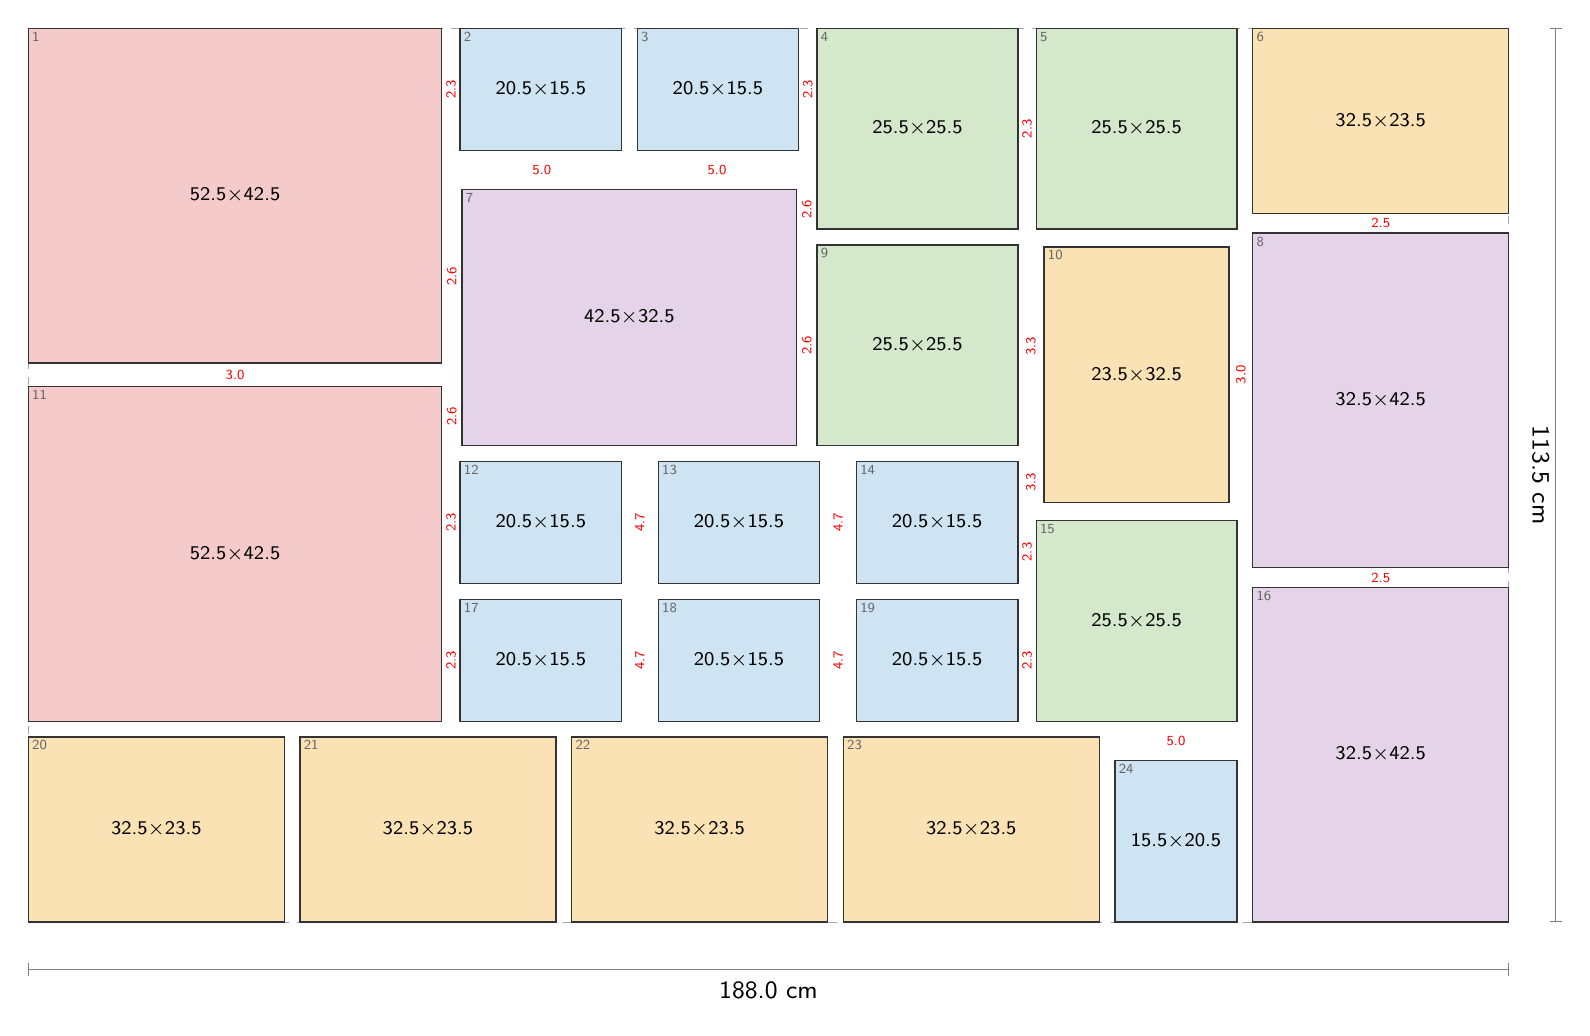
\begin{tikzpicture}[x=1mm, y=-1mm]
\draw[gray!70, dashed, line width=0.4pt] (0,0) rectangle (188.00,113.50);
\filldraw[fill=ft4, draw=black!80, line width=0.5pt] (0.00,0.00) rectangle (52.50,42.50);
\node[align=center, inner sep=0pt] at (26.25,21.25) {\scriptsize 52.5$\times$42.5};
\node[anchor=north west, inner sep=1.2pt, font=\tiny, text=black!60] at (0.00,0.00) {1};
\filldraw[fill=ft0, draw=black!80, line width=0.5pt] (54.83,0.00) rectangle (75.33,15.50);
\node[align=center, inner sep=0pt] at (65.08,7.75) {\scriptsize 20.5$\times$15.5};
\node[anchor=north west, inner sep=1.2pt, font=\tiny, text=black!60] at (54.83,0.00) {2};
\filldraw[fill=ft0, draw=black!80, line width=0.5pt] (77.33,0.00) rectangle (97.83,15.50);
\node[align=center, inner sep=0pt] at (87.58,7.75) {\scriptsize 20.5$\times$15.5};
\node[anchor=north west, inner sep=1.2pt, font=\tiny, text=black!60] at (77.33,0.00) {3};
\filldraw[fill=ft2, draw=black!80, line width=0.5pt] (100.17,0.00) rectangle (125.67,25.50);
\node[align=center, inner sep=0pt] at (112.92,12.75) {\scriptsize 25.5$\times$25.5};
\node[anchor=north west, inner sep=1.2pt, font=\tiny, text=black!60] at (100.17,0.00) {4};
\filldraw[fill=ft2, draw=black!80, line width=0.5pt] (128.00,0.00) rectangle (153.50,25.50);
\node[align=center, inner sep=0pt] at (140.75,12.75) {\scriptsize 25.5$\times$25.5};
\node[anchor=north west, inner sep=1.2pt, font=\tiny, text=black!60] at (128.00,0.00) {5};
\filldraw[fill=ft1, draw=black!80, line width=0.5pt] (155.50,0.00) rectangle (188.00,23.50);
\node[align=center, inner sep=0pt] at (171.75,11.75) {\scriptsize 32.5$\times$23.5};
\node[anchor=north west, inner sep=1.2pt, font=\tiny, text=black!60] at (155.50,0.00) {6};
\filldraw[fill=ft3, draw=black!80, line width=0.5pt] (55.08,20.50) rectangle (97.58,53.00);
\node[align=center, inner sep=0pt] at (76.33,36.75) {\scriptsize 42.5$\times$32.5};
\node[anchor=north west, inner sep=1.2pt, font=\tiny, text=black!60] at (55.08,20.50) {7};
\filldraw[fill=ft3, draw=black!80, line width=0.5pt] (155.50,26.00) rectangle (188.00,68.50);
\node[align=center, inner sep=0pt] at (171.75,47.25) {\scriptsize 32.5$\times$42.5};
\node[anchor=north west, inner sep=1.2pt, font=\tiny, text=black!60] at (155.50,26.00) {8};
\filldraw[fill=ft2, draw=black!80, line width=0.5pt] (100.17,27.50) rectangle (125.67,53.00);
\node[align=center, inner sep=0pt] at (112.92,40.25) {\scriptsize 25.5$\times$25.5};
\node[anchor=north west, inner sep=1.2pt, font=\tiny, text=black!60] at (100.17,27.50) {9};
\filldraw[fill=ft1, draw=black!80, line width=0.5pt] (129.00,27.75) rectangle (152.50,60.25);
\node[align=center, inner sep=0pt] at (140.75,44.00) {\scriptsize 23.5$\times$32.5};
\node[anchor=north west, inner sep=1.2pt, font=\tiny, text=black!60] at (129.00,27.75) {10};
\filldraw[fill=ft4, draw=black!80, line width=0.5pt] (0.00,45.50) rectangle (52.50,88.00);
\node[align=center, inner sep=0pt] at (26.25,66.75) {\scriptsize 52.5$\times$42.5};
\node[anchor=north west, inner sep=1.2pt, font=\tiny, text=black!60] at (0.00,45.50) {11};
\filldraw[fill=ft0, draw=black!80, line width=0.5pt] (54.83,55.00) rectangle (75.33,70.50);
\node[align=center, inner sep=0pt] at (65.08,62.75) {\scriptsize 20.5$\times$15.5};
\node[anchor=north west, inner sep=1.2pt, font=\tiny, text=black!60] at (54.83,55.00) {12};
\filldraw[fill=ft0, draw=black!80, line width=0.5pt] (80.00,55.00) rectangle (100.50,70.50);
\node[align=center, inner sep=0pt] at (90.25,62.75) {\scriptsize 20.5$\times$15.5};
\node[anchor=north west, inner sep=1.2pt, font=\tiny, text=black!60] at (80.00,55.00) {13};
\filldraw[fill=ft0, draw=black!80, line width=0.5pt] (105.17,55.00) rectangle (125.67,70.50);
\node[align=center, inner sep=0pt] at (115.42,62.75) {\scriptsize 20.5$\times$15.5};
\node[anchor=north west, inner sep=1.2pt, font=\tiny, text=black!60] at (105.17,55.00) {14};
\filldraw[fill=ft2, draw=black!80, line width=0.5pt] (128.00,62.50) rectangle (153.50,88.00);
\node[align=center, inner sep=0pt] at (140.75,75.25) {\scriptsize 25.5$\times$25.5};
\node[anchor=north west, inner sep=1.2pt, font=\tiny, text=black!60] at (128.00,62.50) {15};
\filldraw[fill=ft3, draw=black!80, line width=0.5pt] (155.50,71.00) rectangle (188.00,113.50);
\node[align=center, inner sep=0pt] at (171.75,92.25) {\scriptsize 32.5$\times$42.5};
\node[anchor=north west, inner sep=1.2pt, font=\tiny, text=black!60] at (155.50,71.00) {16};
\filldraw[fill=ft0, draw=black!80, line width=0.5pt] (54.83,72.50) rectangle (75.33,88.00);
\node[align=center, inner sep=0pt] at (65.08,80.25) {\scriptsize 20.5$\times$15.5};
\node[anchor=north west, inner sep=1.2pt, font=\tiny, text=black!60] at (54.83,72.50) {17};
\filldraw[fill=ft0, draw=black!80, line width=0.5pt] (80.00,72.50) rectangle (100.50,88.00);
\node[align=center, inner sep=0pt] at (90.25,80.25) {\scriptsize 20.5$\times$15.5};
\node[anchor=north west, inner sep=1.2pt, font=\tiny, text=black!60] at (80.00,72.50) {18};
\filldraw[fill=ft0, draw=black!80, line width=0.5pt] (105.17,72.50) rectangle (125.67,88.00);
\node[align=center, inner sep=0pt] at (115.42,80.25) {\scriptsize 20.5$\times$15.5};
\node[anchor=north west, inner sep=1.2pt, font=\tiny, text=black!60] at (105.17,72.50) {19};
\filldraw[fill=ft1, draw=black!80, line width=0.5pt] (0.00,90.00) rectangle (32.50,113.50);
\node[align=center, inner sep=0pt] at (16.25,101.75) {\scriptsize 32.5$\times$23.5};
\node[anchor=north west, inner sep=1.2pt, font=\tiny, text=black!60] at (0.00,90.00) {20};
\filldraw[fill=ft1, draw=black!80, line width=0.5pt] (34.50,90.00) rectangle (67.00,113.50);
\node[align=center, inner sep=0pt] at (50.75,101.75) {\scriptsize 32.5$\times$23.5};
\node[anchor=north west, inner sep=1.2pt, font=\tiny, text=black!60] at (34.50,90.00) {21};
\filldraw[fill=ft1, draw=black!80, line width=0.5pt] (69.00,90.00) rectangle (101.50,113.50);
\node[align=center, inner sep=0pt] at (85.25,101.75) {\scriptsize 32.5$\times$23.5};
\node[anchor=north west, inner sep=1.2pt, font=\tiny, text=black!60] at (69.00,90.00) {22};
\filldraw[fill=ft1, draw=black!80, line width=0.5pt] (103.50,90.00) rectangle (136.00,113.50);
\node[align=center, inner sep=0pt] at (119.75,101.75) {\scriptsize 32.5$\times$23.5};
\node[anchor=north west, inner sep=1.2pt, font=\tiny, text=black!60] at (103.50,90.00) {23};
\filldraw[fill=ft0, draw=black!80, line width=0.5pt] (138.00,93.00) rectangle (153.50,113.50);
\node[align=center, inner sep=0pt] at (145.75,103.25) {\scriptsize 15.5$\times$20.5};
\node[anchor=north west, inner sep=1.2pt, font=\tiny, text=black!60] at (138.00,93.00) {24};
\node[font=\tiny, text=red, fill=white, inner sep=0.3pt, rotate=90] at (53.67,7.75) {2.3};
\node[font=\tiny, text=red, fill=white, inner sep=0.3pt, rotate=90] at (53.79,31.50) {2.6};
\node[font=\tiny, text=red, fill=white, inner sep=0.3pt] at (26.25,44.00) {3.0};
\node[font=\tiny, text=red, fill=white, inner sep=0.3pt] at (65.21,18.00) {5.0};
\node[font=\tiny, text=red, fill=white, inner sep=0.3pt, rotate=90] at (99.00,7.75) {2.3};
\node[font=\tiny, text=red, fill=white, inner sep=0.3pt] at (87.46,18.00) {5.0};
\node[font=\tiny, text=red, fill=white, inner sep=0.3pt, rotate=90] at (126.83,12.75) {2.3};
\node[font=\tiny, text=red, fill=white, inner sep=0.3pt] at (171.75,24.75) {2.5};
\node[font=\tiny, text=red, fill=white, inner sep=0.3pt, rotate=90] at (98.88,23.00) {2.6};
\node[font=\tiny, text=red, fill=white, inner sep=0.3pt, rotate=90] at (98.88,40.25) {2.6};
\node[font=\tiny, text=red, fill=white, inner sep=0.3pt] at (171.75,69.75) {2.5};
\node[font=\tiny, text=red, fill=white, inner sep=0.3pt, rotate=90] at (127.33,40.38) {3.3};
\node[font=\tiny, text=red, fill=white, inner sep=0.3pt, rotate=90] at (154.00,44.00) {3.0};
\node[font=\tiny, text=red, fill=white, inner sep=0.3pt, rotate=90] at (53.79,49.25) {2.6};
\node[font=\tiny, text=red, fill=white, inner sep=0.3pt, rotate=90] at (53.67,62.75) {2.3};
\node[font=\tiny, text=red, fill=white, inner sep=0.3pt, rotate=90] at (53.67,80.25) {2.3};
\node[font=\tiny, text=red, fill=white, inner sep=0.3pt, rotate=90] at (77.67,62.75) {4.7};
\node[font=\tiny, text=red, fill=white, inner sep=0.3pt, rotate=90] at (102.83,62.75) {4.7};
\node[font=\tiny, text=red, fill=white, inner sep=0.3pt, rotate=90] at (127.33,57.62) {3.3};
\node[font=\tiny, text=red, fill=white, inner sep=0.3pt, rotate=90] at (126.83,66.50) {2.3};
\node[font=\tiny, text=red, fill=white, inner sep=0.3pt] at (145.75,90.50) {5.0};
\node[font=\tiny, text=red, fill=white, inner sep=0.3pt, rotate=90] at (77.67,80.25) {4.7};
\node[font=\tiny, text=red, fill=white, inner sep=0.3pt, rotate=90] at (102.83,80.25) {4.7};
\node[font=\tiny, text=red, fill=white, inner sep=0.3pt, rotate=90] at (126.83,80.25) {2.3};
\draw[Bar-Bar, gray] (0,119.50) -- (188.00,119.50) node[midway, below=1pt, font=\small, text=black] {188.0 cm};
\draw[Bar-Bar, gray] (194.00,0) -- (194.00,113.50) node[midway, right=1pt, font=\small, text=black, rotate=-90, anchor=north] {113.5 cm};
\end{tikzpicture}\\[4pt]
{\scriptsize Scale 1:10 (1 mm = 1 cm). Red numbers mark gaps that deviate from the nominal gap by more than 0.25 cm. Small grey numbers index the coordinate table.}
\end{minipage}\hfill
\begin{minipage}[t]{0.25\textwidth}\vspace{0pt}
\small
\begin{tabular}{@{}l l@{}}
\toprule
Outer size & 188.0 $\times$ 113.5 cm \\
Nominal gap & 2 cm \\
Actual gaps & 2.0 -- 5.0 cm \\
Max.\ deviation & 3.0 cm \\
Mean deviation & 0.62 cm \\
Border notches & none \\
Corners filled & 4 / 4 \\
Frames used & 24 of 28 \\
\bottomrule
\end{tabular}

\vspace{8pt}
\scriptsize
\begin{tabular}{@{}c l l r r@{}}
\toprule
 & outer w $\times$ h (cm) & & used & have \\
\midrule
\tikz[baseline=-0.6ex]\fill[ft0,draw=black!60] (0,0) rectangle (1.2ex,1.2ex); & 20.5$\times$15.5 & L & 8 & 9 \\
\tikz[baseline=-0.6ex]\fill[ft0,draw=black!60] (0,0) rectangle (1.2ex,1.2ex); & 15.5$\times$20.5 & P & 1 & 2 \\
\tikz[baseline=-0.6ex]\fill[ft3,draw=black!60] (0,0) rectangle (1.2ex,1.2ex); & 32.5$\times$42.5 & P & 2 & 2 \\
\tikz[baseline=-0.6ex]\fill[ft3,draw=black!60] (0,0) rectangle (1.2ex,1.2ex); & 42.5$\times$32.5 & L & 1 & 1 \\
\tikz[baseline=-0.6ex]\fill[ft1,draw=black!60] (0,0) rectangle (1.2ex,1.2ex); & 32.5$\times$23.5 & L & 5 & 5 \\
\tikz[baseline=-0.6ex]\fill[ft1,draw=black!60] (0,0) rectangle (1.2ex,1.2ex); & 23.5$\times$32.5 & P & 1 & 1 \\
\tikz[baseline=-0.6ex]\fill[ft2,draw=black!60] (0,0) rectangle (1.2ex,1.2ex); & 25.5$\times$25.5 &  & 4 & 5 \\
\tikz[baseline=-0.6ex]\fill[ft4,draw=black!60] (0,0) rectangle (1.2ex,1.2ex); & 42.5$\times$52.5 & P & 0 & 1 \\
\tikz[baseline=-0.6ex]\fill[ft4,draw=black!60] (0,0) rectangle (1.2ex,1.2ex); & 52.5$\times$42.5 & L & 2 & 2 \\
\bottomrule
\end{tabular}

\vspace{8pt}
{\bfseries Positions} (top-left corner, cm)\\[2pt]
\tiny
\begin{tabular}{@{}r l r r@{}}
\toprule
\# & frame w $\times$ h & x & y \\
\midrule
1 & 52.5 $\times$ 42.5 & 0.0 & 0.0 \\
2 & 20.5 $\times$ 15.5 & 54.8 & 0.0 \\
3 & 20.5 $\times$ 15.5 & 77.3 & 0.0 \\
4 & 25.5 $\times$ 25.5 & 100.2 & 0.0 \\
5 & 25.5 $\times$ 25.5 & 128.0 & 0.0 \\
6 & 32.5 $\times$ 23.5 & 155.5 & 0.0 \\
7 & 42.5 $\times$ 32.5 & 55.1 & 20.5 \\
8 & 32.5 $\times$ 42.5 & 155.5 & 26.0 \\
9 & 25.5 $\times$ 25.5 & 100.2 & 27.5 \\
10 & 23.5 $\times$ 32.5 & 129.0 & 27.8 \\
11 & 52.5 $\times$ 42.5 & 0.0 & 45.5 \\
12 & 20.5 $\times$ 15.5 & 54.8 & 55.0 \\
13 & 20.5 $\times$ 15.5 & 80.0 & 55.0 \\
14 & 20.5 $\times$ 15.5 & 105.2 & 55.0 \\
15 & 25.5 $\times$ 25.5 & 128.0 & 62.5 \\
16 & 32.5 $\times$ 42.5 & 155.5 & 71.0 \\
17 & 20.5 $\times$ 15.5 & 54.8 & 72.5 \\
18 & 20.5 $\times$ 15.5 & 80.0 & 72.5 \\
19 & 20.5 $\times$ 15.5 & 105.2 & 72.5 \\
20 & 32.5 $\times$ 23.5 & 0.0 & 90.0 \\
21 & 32.5 $\times$ 23.5 & 34.5 & 90.0 \\
22 & 32.5 $\times$ 23.5 & 69.0 & 90.0 \\
23 & 32.5 $\times$ 23.5 & 103.5 & 90.0 \\
24 & 15.5 $\times$ 20.5 & 138.0 & 93.0 \\
\bottomrule
\end{tabular}
\end{minipage}
\clearpage

\begin{minipage}[t]{0.74\textwidth}\vspace{0pt}
{\LARGE\bfseries Layout 2}\hspace{1.5em}{\large 167.5 $\times$ 130.5 cm \quad gap 3.5 cm \quad 24 frames}\\[8pt]
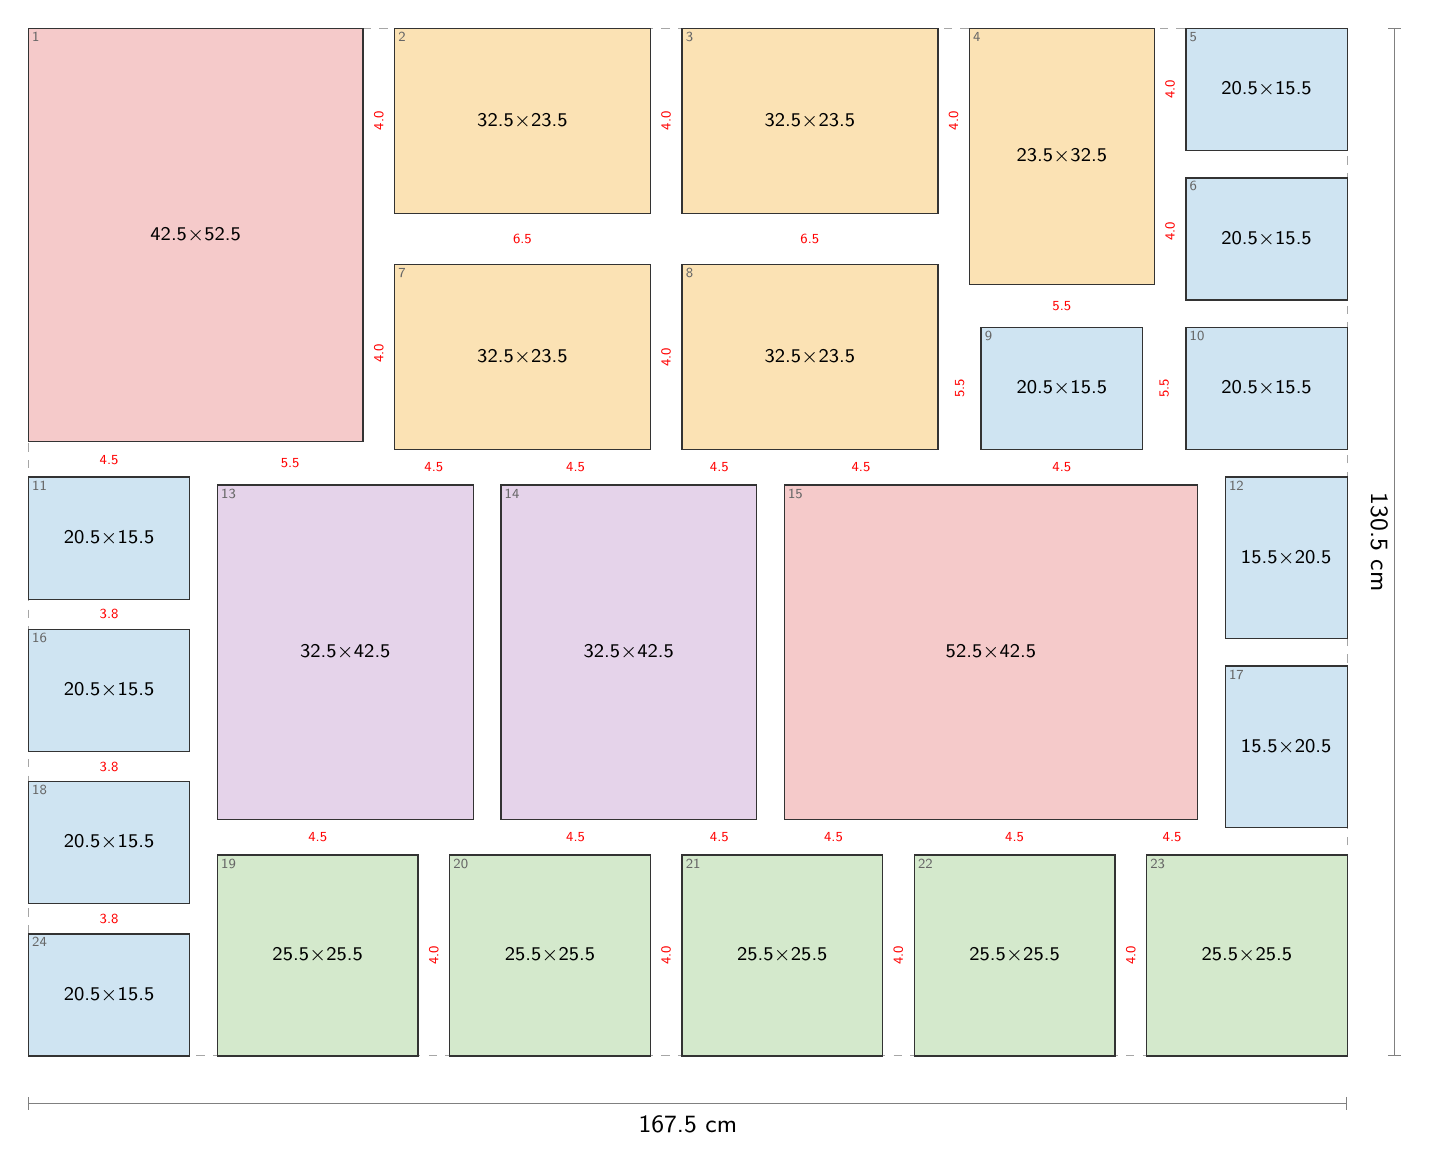
\begin{tikzpicture}[x=1mm, y=-1mm]
\draw[gray!70, dashed, line width=0.4pt] (0,0) rectangle (167.50,130.50);
\filldraw[fill=ft4, draw=black!80, line width=0.5pt] (0.00,0.00) rectangle (42.50,52.50);
\node[align=center, inner sep=0pt] at (21.25,26.25) {\scriptsize 42.5$\times$52.5};
\node[anchor=north west, inner sep=1.2pt, font=\tiny, text=black!60] at (0.00,0.00) {1};
\filldraw[fill=ft1, draw=black!80, line width=0.5pt] (46.50,0.00) rectangle (79.00,23.50);
\node[align=center, inner sep=0pt] at (62.75,11.75) {\scriptsize 32.5$\times$23.5};
\node[anchor=north west, inner sep=1.2pt, font=\tiny, text=black!60] at (46.50,0.00) {2};
\filldraw[fill=ft1, draw=black!80, line width=0.5pt] (83.00,0.00) rectangle (115.50,23.50);
\node[align=center, inner sep=0pt] at (99.25,11.75) {\scriptsize 32.5$\times$23.5};
\node[anchor=north west, inner sep=1.2pt, font=\tiny, text=black!60] at (83.00,0.00) {3};
\filldraw[fill=ft1, draw=black!80, line width=0.5pt] (119.50,0.00) rectangle (143.00,32.50);
\node[align=center, inner sep=0pt] at (131.25,16.25) {\scriptsize 23.5$\times$32.5};
\node[anchor=north west, inner sep=1.2pt, font=\tiny, text=black!60] at (119.50,0.00) {4};
\filldraw[fill=ft0, draw=black!80, line width=0.5pt] (147.00,0.00) rectangle (167.50,15.50);
\node[align=center, inner sep=0pt] at (157.25,7.75) {\scriptsize 20.5$\times$15.5};
\node[anchor=north west, inner sep=1.2pt, font=\tiny, text=black!60] at (147.00,0.00) {5};
\filldraw[fill=ft0, draw=black!80, line width=0.5pt] (147.00,19.00) rectangle (167.50,34.50);
\node[align=center, inner sep=0pt] at (157.25,26.75) {\scriptsize 20.5$\times$15.5};
\node[anchor=north west, inner sep=1.2pt, font=\tiny, text=black!60] at (147.00,19.00) {6};
\filldraw[fill=ft1, draw=black!80, line width=0.5pt] (46.50,30.00) rectangle (79.00,53.50);
\node[align=center, inner sep=0pt] at (62.75,41.75) {\scriptsize 32.5$\times$23.5};
\node[anchor=north west, inner sep=1.2pt, font=\tiny, text=black!60] at (46.50,30.00) {7};
\filldraw[fill=ft1, draw=black!80, line width=0.5pt] (83.00,30.00) rectangle (115.50,53.50);
\node[align=center, inner sep=0pt] at (99.25,41.75) {\scriptsize 32.5$\times$23.5};
\node[anchor=north west, inner sep=1.2pt, font=\tiny, text=black!60] at (83.00,30.00) {8};
\filldraw[fill=ft0, draw=black!80, line width=0.5pt] (121.00,38.00) rectangle (141.50,53.50);
\node[align=center, inner sep=0pt] at (131.25,45.75) {\scriptsize 20.5$\times$15.5};
\node[anchor=north west, inner sep=1.2pt, font=\tiny, text=black!60] at (121.00,38.00) {9};
\filldraw[fill=ft0, draw=black!80, line width=0.5pt] (147.00,38.00) rectangle (167.50,53.50);
\node[align=center, inner sep=0pt] at (157.25,45.75) {\scriptsize 20.5$\times$15.5};
\node[anchor=north west, inner sep=1.2pt, font=\tiny, text=black!60] at (147.00,38.00) {10};
\filldraw[fill=ft0, draw=black!80, line width=0.5pt] (0.00,57.00) rectangle (20.50,72.50);
\node[align=center, inner sep=0pt] at (10.25,64.75) {\scriptsize 20.5$\times$15.5};
\node[anchor=north west, inner sep=1.2pt, font=\tiny, text=black!60] at (0.00,57.00) {11};
\filldraw[fill=ft0, draw=black!80, line width=0.5pt] (152.00,57.00) rectangle (167.50,77.50);
\node[align=center, inner sep=0pt] at (159.75,67.25) {\scriptsize 15.5$\times$20.5};
\node[anchor=north west, inner sep=1.2pt, font=\tiny, text=black!60] at (152.00,57.00) {12};
\filldraw[fill=ft3, draw=black!80, line width=0.5pt] (24.00,58.00) rectangle (56.50,100.50);
\node[align=center, inner sep=0pt] at (40.25,79.25) {\scriptsize 32.5$\times$42.5};
\node[anchor=north west, inner sep=1.2pt, font=\tiny, text=black!60] at (24.00,58.00) {13};
\filldraw[fill=ft3, draw=black!80, line width=0.5pt] (60.00,58.00) rectangle (92.50,100.50);
\node[align=center, inner sep=0pt] at (76.25,79.25) {\scriptsize 32.5$\times$42.5};
\node[anchor=north west, inner sep=1.2pt, font=\tiny, text=black!60] at (60.00,58.00) {14};
\filldraw[fill=ft4, draw=black!80, line width=0.5pt] (96.00,58.00) rectangle (148.50,100.50);
\node[align=center, inner sep=0pt] at (122.25,79.25) {\scriptsize 52.5$\times$42.5};
\node[anchor=north west, inner sep=1.2pt, font=\tiny, text=black!60] at (96.00,58.00) {15};
\filldraw[fill=ft0, draw=black!80, line width=0.5pt] (0.00,76.33) rectangle (20.50,91.83);
\node[align=center, inner sep=0pt] at (10.25,84.08) {\scriptsize 20.5$\times$15.5};
\node[anchor=north west, inner sep=1.2pt, font=\tiny, text=black!60] at (0.00,76.33) {16};
\filldraw[fill=ft0, draw=black!80, line width=0.5pt] (152.00,81.00) rectangle (167.50,101.50);
\node[align=center, inner sep=0pt] at (159.75,91.25) {\scriptsize 15.5$\times$20.5};
\node[anchor=north west, inner sep=1.2pt, font=\tiny, text=black!60] at (152.00,81.00) {17};
\filldraw[fill=ft0, draw=black!80, line width=0.5pt] (0.00,95.67) rectangle (20.50,111.17);
\node[align=center, inner sep=0pt] at (10.25,103.42) {\scriptsize 20.5$\times$15.5};
\node[anchor=north west, inner sep=1.2pt, font=\tiny, text=black!60] at (0.00,95.67) {18};
\filldraw[fill=ft2, draw=black!80, line width=0.5pt] (24.00,105.00) rectangle (49.50,130.50);
\node[align=center, inner sep=0pt] at (36.75,117.75) {\scriptsize 25.5$\times$25.5};
\node[anchor=north west, inner sep=1.2pt, font=\tiny, text=black!60] at (24.00,105.00) {19};
\filldraw[fill=ft2, draw=black!80, line width=0.5pt] (53.50,105.00) rectangle (79.00,130.50);
\node[align=center, inner sep=0pt] at (66.25,117.75) {\scriptsize 25.5$\times$25.5};
\node[anchor=north west, inner sep=1.2pt, font=\tiny, text=black!60] at (53.50,105.00) {20};
\filldraw[fill=ft2, draw=black!80, line width=0.5pt] (83.00,105.00) rectangle (108.50,130.50);
\node[align=center, inner sep=0pt] at (95.75,117.75) {\scriptsize 25.5$\times$25.5};
\node[anchor=north west, inner sep=1.2pt, font=\tiny, text=black!60] at (83.00,105.00) {21};
\filldraw[fill=ft2, draw=black!80, line width=0.5pt] (112.50,105.00) rectangle (138.00,130.50);
\node[align=center, inner sep=0pt] at (125.25,117.75) {\scriptsize 25.5$\times$25.5};
\node[anchor=north west, inner sep=1.2pt, font=\tiny, text=black!60] at (112.50,105.00) {22};
\filldraw[fill=ft2, draw=black!80, line width=0.5pt] (142.00,105.00) rectangle (167.50,130.50);
\node[align=center, inner sep=0pt] at (154.75,117.75) {\scriptsize 25.5$\times$25.5};
\node[anchor=north west, inner sep=1.2pt, font=\tiny, text=black!60] at (142.00,105.00) {23};
\filldraw[fill=ft0, draw=black!80, line width=0.5pt] (0.00,115.00) rectangle (20.50,130.50);
\node[align=center, inner sep=0pt] at (10.25,122.75) {\scriptsize 20.5$\times$15.5};
\node[anchor=north west, inner sep=1.2pt, font=\tiny, text=black!60] at (0.00,115.00) {24};
\node[font=\tiny, text=red, fill=white, inner sep=0.3pt, rotate=90] at (44.50,11.75) {4.0};
\node[font=\tiny, text=red, fill=white, inner sep=0.3pt, rotate=90] at (44.50,41.25) {4.0};
\node[font=\tiny, text=red, fill=white, inner sep=0.3pt] at (10.25,54.75) {4.5};
\node[font=\tiny, text=red, fill=white, inner sep=0.3pt] at (33.25,55.25) {5.5};
\node[font=\tiny, text=red, fill=white, inner sep=0.3pt, rotate=90] at (81.00,11.75) {4.0};
\node[font=\tiny, text=red, fill=white, inner sep=0.3pt] at (62.75,26.75) {6.5};
\node[font=\tiny, text=red, fill=white, inner sep=0.3pt, rotate=90] at (117.50,11.75) {4.0};
\node[font=\tiny, text=red, fill=white, inner sep=0.3pt] at (99.25,26.75) {6.5};
\node[font=\tiny, text=red, fill=white, inner sep=0.3pt, rotate=90] at (145.00,7.75) {4.0};
\node[font=\tiny, text=red, fill=white, inner sep=0.3pt, rotate=90] at (145.00,25.75) {4.0};
\node[font=\tiny, text=red, fill=white, inner sep=0.3pt] at (131.25,35.25) {5.5};
\node[font=\tiny, text=red, fill=white, inner sep=0.3pt, rotate=90] at (81.00,41.75) {4.0};
\node[font=\tiny, text=red, fill=white, inner sep=0.3pt] at (51.50,55.75) {4.5};
\node[font=\tiny, text=red, fill=white, inner sep=0.3pt] at (69.50,55.75) {4.5};
\node[font=\tiny, text=red, fill=white, inner sep=0.3pt, rotate=90] at (118.25,45.75) {5.5};
\node[font=\tiny, text=red, fill=white, inner sep=0.3pt] at (87.75,55.75) {4.5};
\node[font=\tiny, text=red, fill=white, inner sep=0.3pt] at (105.75,55.75) {4.5};
\node[font=\tiny, text=red, fill=white, inner sep=0.3pt, rotate=90] at (144.25,45.75) {5.5};
\node[font=\tiny, text=red, fill=white, inner sep=0.3pt] at (131.25,55.75) {4.5};
\node[font=\tiny, text=red, fill=white, inner sep=0.3pt] at (10.25,74.42) {3.8};
\node[font=\tiny, text=red, fill=white, inner sep=0.3pt] at (36.75,102.75) {4.5};
\node[font=\tiny, text=red, fill=white, inner sep=0.3pt] at (69.50,102.75) {4.5};
\node[font=\tiny, text=red, fill=white, inner sep=0.3pt] at (87.75,102.75) {4.5};
\node[font=\tiny, text=red, fill=white, inner sep=0.3pt] at (102.25,102.75) {4.5};
\node[font=\tiny, text=red, fill=white, inner sep=0.3pt] at (125.25,102.75) {4.5};
\node[font=\tiny, text=red, fill=white, inner sep=0.3pt] at (145.25,102.75) {4.5};
\node[font=\tiny, text=red, fill=white, inner sep=0.3pt] at (10.25,93.75) {3.8};
\node[font=\tiny, text=red, fill=white, inner sep=0.3pt] at (10.25,113.08) {3.8};
\node[font=\tiny, text=red, fill=white, inner sep=0.3pt, rotate=90] at (51.50,117.75) {4.0};
\node[font=\tiny, text=red, fill=white, inner sep=0.3pt, rotate=90] at (81.00,117.75) {4.0};
\node[font=\tiny, text=red, fill=white, inner sep=0.3pt, rotate=90] at (110.50,117.75) {4.0};
\node[font=\tiny, text=red, fill=white, inner sep=0.3pt, rotate=90] at (140.00,117.75) {4.0};
\draw[Bar-Bar, gray] (0,136.50) -- (167.50,136.50) node[midway, below=1pt, font=\small, text=black] {167.5 cm};
\draw[Bar-Bar, gray] (173.50,0) -- (173.50,130.50) node[midway, right=1pt, font=\small, text=black, rotate=-90, anchor=north] {130.5 cm};
\end{tikzpicture}\\[4pt]
{\scriptsize Scale 1:10 (1 mm = 1 cm). Red numbers mark gaps that deviate from the nominal gap by more than 0.25 cm. Small grey numbers index the coordinate table.}
\end{minipage}\hfill
\begin{minipage}[t]{0.25\textwidth}\vspace{0pt}
\small
\begin{tabular}{@{}l l@{}}
\toprule
Outer size & 167.5 $\times$ 130.5 cm \\
Nominal gap & 3.5 cm \\
Actual gaps & 3.5 -- 6.5 cm \\
Max.\ deviation & 3.0 cm \\
Mean deviation & 0.72 cm \\
Border notches & none \\
Corners filled & 4 / 4 \\
Frames used & 24 of 28 \\
\bottomrule
\end{tabular}

\vspace{8pt}
\scriptsize
\begin{tabular}{@{}c l l r r@{}}
\toprule
 & outer w $\times$ h (cm) & & used & have \\
\midrule
\tikz[baseline=-0.6ex]\fill[ft0,draw=black!60] (0,0) rectangle (1.2ex,1.2ex); & 20.5$\times$15.5 & L & 8 & 9 \\
\tikz[baseline=-0.6ex]\fill[ft0,draw=black!60] (0,0) rectangle (1.2ex,1.2ex); & 15.5$\times$20.5 & P & 2 & 2 \\
\tikz[baseline=-0.6ex]\fill[ft3,draw=black!60] (0,0) rectangle (1.2ex,1.2ex); & 32.5$\times$42.5 & P & 2 & 2 \\
\tikz[baseline=-0.6ex]\fill[ft3,draw=black!60] (0,0) rectangle (1.2ex,1.2ex); & 42.5$\times$32.5 & L & 0 & 1 \\
\tikz[baseline=-0.6ex]\fill[ft1,draw=black!60] (0,0) rectangle (1.2ex,1.2ex); & 32.5$\times$23.5 & L & 4 & 5 \\
\tikz[baseline=-0.6ex]\fill[ft1,draw=black!60] (0,0) rectangle (1.2ex,1.2ex); & 23.5$\times$32.5 & P & 1 & 1 \\
\tikz[baseline=-0.6ex]\fill[ft2,draw=black!60] (0,0) rectangle (1.2ex,1.2ex); & 25.5$\times$25.5 &  & 5 & 5 \\
\tikz[baseline=-0.6ex]\fill[ft4,draw=black!60] (0,0) rectangle (1.2ex,1.2ex); & 42.5$\times$52.5 & P & 1 & 1 \\
\tikz[baseline=-0.6ex]\fill[ft4,draw=black!60] (0,0) rectangle (1.2ex,1.2ex); & 52.5$\times$42.5 & L & 1 & 2 \\
\bottomrule
\end{tabular}

\vspace{8pt}
{\bfseries Positions} (top-left corner, cm)\\[2pt]
\tiny
\begin{tabular}{@{}r l r r@{}}
\toprule
\# & frame w $\times$ h & x & y \\
\midrule
1 & 42.5 $\times$ 52.5 & 0.0 & 0.0 \\
2 & 32.5 $\times$ 23.5 & 46.5 & 0.0 \\
3 & 32.5 $\times$ 23.5 & 83.0 & 0.0 \\
4 & 23.5 $\times$ 32.5 & 119.5 & 0.0 \\
5 & 20.5 $\times$ 15.5 & 147.0 & 0.0 \\
6 & 20.5 $\times$ 15.5 & 147.0 & 19.0 \\
7 & 32.5 $\times$ 23.5 & 46.5 & 30.0 \\
8 & 32.5 $\times$ 23.5 & 83.0 & 30.0 \\
9 & 20.5 $\times$ 15.5 & 121.0 & 38.0 \\
10 & 20.5 $\times$ 15.5 & 147.0 & 38.0 \\
11 & 20.5 $\times$ 15.5 & 0.0 & 57.0 \\
12 & 15.5 $\times$ 20.5 & 152.0 & 57.0 \\
13 & 32.5 $\times$ 42.5 & 24.0 & 58.0 \\
14 & 32.5 $\times$ 42.5 & 60.0 & 58.0 \\
15 & 52.5 $\times$ 42.5 & 96.0 & 58.0 \\
16 & 20.5 $\times$ 15.5 & 0.0 & 76.3 \\
17 & 15.5 $\times$ 20.5 & 152.0 & 81.0 \\
18 & 20.5 $\times$ 15.5 & 0.0 & 95.7 \\
19 & 25.5 $\times$ 25.5 & 24.0 & 105.0 \\
20 & 25.5 $\times$ 25.5 & 53.5 & 105.0 \\
21 & 25.5 $\times$ 25.5 & 83.0 & 105.0 \\
22 & 25.5 $\times$ 25.5 & 112.5 & 105.0 \\
23 & 25.5 $\times$ 25.5 & 142.0 & 105.0 \\
24 & 20.5 $\times$ 15.5 & 0.0 & 115.0 \\
\bottomrule
\end{tabular}
\end{minipage}
\clearpage

\begin{minipage}[t]{0.74\textwidth}\vspace{0pt}
{\LARGE\bfseries Layout 3}\hspace{1.5em}{\large 183.5 $\times$ 115.0 cm \quad gap 2 cm \quad 23 frames}\\[8pt]
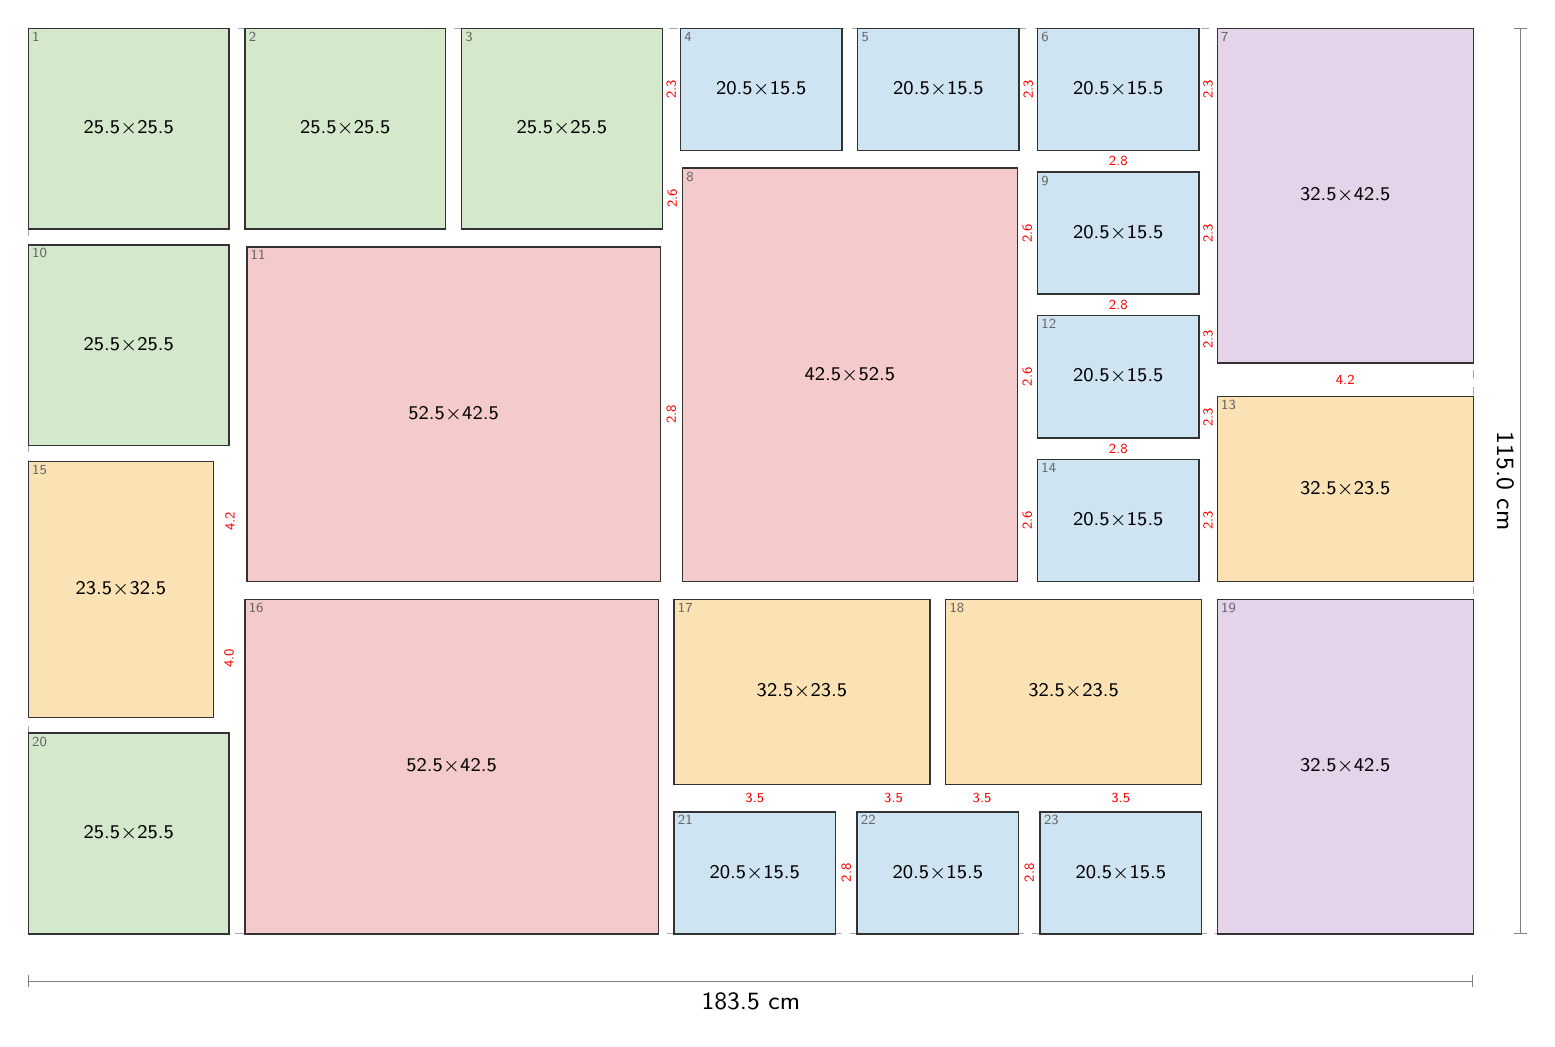
\begin{tikzpicture}[x=1mm, y=-1mm]
\draw[gray!70, dashed, line width=0.4pt] (0,0) rectangle (183.50,115.00);
\filldraw[fill=ft2, draw=black!80, line width=0.5pt] (0.00,0.00) rectangle (25.50,25.50);
\node[align=center, inner sep=0pt] at (12.75,12.75) {\scriptsize 25.5$\times$25.5};
\node[anchor=north west, inner sep=1.2pt, font=\tiny, text=black!60] at (0.00,0.00) {1};
\filldraw[fill=ft2, draw=black!80, line width=0.5pt] (27.50,0.00) rectangle (53.00,25.50);
\node[align=center, inner sep=0pt] at (40.25,12.75) {\scriptsize 25.5$\times$25.5};
\node[anchor=north west, inner sep=1.2pt, font=\tiny, text=black!60] at (27.50,0.00) {2};
\filldraw[fill=ft2, draw=black!80, line width=0.5pt] (55.00,0.00) rectangle (80.50,25.50);
\node[align=center, inner sep=0pt] at (67.75,12.75) {\scriptsize 25.5$\times$25.5};
\node[anchor=north west, inner sep=1.2pt, font=\tiny, text=black!60] at (55.00,0.00) {3};
\filldraw[fill=ft0, draw=black!80, line width=0.5pt] (82.83,0.00) rectangle (103.33,15.50);
\node[align=center, inner sep=0pt] at (93.08,7.75) {\scriptsize 20.5$\times$15.5};
\node[anchor=north west, inner sep=1.2pt, font=\tiny, text=black!60] at (82.83,0.00) {4};
\filldraw[fill=ft0, draw=black!80, line width=0.5pt] (105.33,0.00) rectangle (125.83,15.50);
\node[align=center, inner sep=0pt] at (115.58,7.75) {\scriptsize 20.5$\times$15.5};
\node[anchor=north west, inner sep=1.2pt, font=\tiny, text=black!60] at (105.33,0.00) {5};
\filldraw[fill=ft0, draw=black!80, line width=0.5pt] (128.17,0.00) rectangle (148.67,15.50);
\node[align=center, inner sep=0pt] at (138.42,7.75) {\scriptsize 20.5$\times$15.5};
\node[anchor=north west, inner sep=1.2pt, font=\tiny, text=black!60] at (128.17,0.00) {6};
\filldraw[fill=ft3, draw=black!80, line width=0.5pt] (151.00,0.00) rectangle (183.50,42.50);
\node[align=center, inner sep=0pt] at (167.25,21.25) {\scriptsize 32.5$\times$42.5};
\node[anchor=north west, inner sep=1.2pt, font=\tiny, text=black!60] at (151.00,0.00) {7};
\filldraw[fill=ft4, draw=black!80, line width=0.5pt] (83.08,17.75) rectangle (125.58,70.25);
\node[align=center, inner sep=0pt] at (104.33,44.00) {\scriptsize 42.5$\times$52.5};
\node[anchor=north west, inner sep=1.2pt, font=\tiny, text=black!60] at (83.08,17.75) {8};
\filldraw[fill=ft0, draw=black!80, line width=0.5pt] (128.17,18.25) rectangle (148.67,33.75);
\node[align=center, inner sep=0pt] at (138.42,26.00) {\scriptsize 20.5$\times$15.5};
\node[anchor=north west, inner sep=1.2pt, font=\tiny, text=black!60] at (128.17,18.25) {9};
\filldraw[fill=ft2, draw=black!80, line width=0.5pt] (0.00,27.50) rectangle (25.50,53.00);
\node[align=center, inner sep=0pt] at (12.75,40.25) {\scriptsize 25.5$\times$25.5};
\node[anchor=north west, inner sep=1.2pt, font=\tiny, text=black!60] at (0.00,27.50) {10};
\filldraw[fill=ft4, draw=black!80, line width=0.5pt] (27.75,27.75) rectangle (80.25,70.25);
\node[align=center, inner sep=0pt] at (54.00,49.00) {\scriptsize 52.5$\times$42.5};
\node[anchor=north west, inner sep=1.2pt, font=\tiny, text=black!60] at (27.75,27.75) {11};
\filldraw[fill=ft0, draw=black!80, line width=0.5pt] (128.17,36.50) rectangle (148.67,52.00);
\node[align=center, inner sep=0pt] at (138.42,44.25) {\scriptsize 20.5$\times$15.5};
\node[anchor=north west, inner sep=1.2pt, font=\tiny, text=black!60] at (128.17,36.50) {12};
\filldraw[fill=ft1, draw=black!80, line width=0.5pt] (151.00,46.75) rectangle (183.50,70.25);
\node[align=center, inner sep=0pt] at (167.25,58.50) {\scriptsize 32.5$\times$23.5};
\node[anchor=north west, inner sep=1.2pt, font=\tiny, text=black!60] at (151.00,46.75) {13};
\filldraw[fill=ft0, draw=black!80, line width=0.5pt] (128.17,54.75) rectangle (148.67,70.25);
\node[align=center, inner sep=0pt] at (138.42,62.50) {\scriptsize 20.5$\times$15.5};
\node[anchor=north west, inner sep=1.2pt, font=\tiny, text=black!60] at (128.17,54.75) {14};
\filldraw[fill=ft1, draw=black!80, line width=0.5pt] (0.00,55.00) rectangle (23.50,87.50);
\node[align=center, inner sep=0pt] at (11.75,71.25) {\scriptsize 23.5$\times$32.5};
\node[anchor=north west, inner sep=1.2pt, font=\tiny, text=black!60] at (0.00,55.00) {15};
\filldraw[fill=ft4, draw=black!80, line width=0.5pt] (27.50,72.50) rectangle (80.00,115.00);
\node[align=center, inner sep=0pt] at (53.75,93.75) {\scriptsize 52.5$\times$42.5};
\node[anchor=north west, inner sep=1.2pt, font=\tiny, text=black!60] at (27.50,72.50) {16};
\filldraw[fill=ft1, draw=black!80, line width=0.5pt] (82.00,72.50) rectangle (114.50,96.00);
\node[align=center, inner sep=0pt] at (98.25,84.25) {\scriptsize 32.5$\times$23.5};
\node[anchor=north west, inner sep=1.2pt, font=\tiny, text=black!60] at (82.00,72.50) {17};
\filldraw[fill=ft1, draw=black!80, line width=0.5pt] (116.50,72.50) rectangle (149.00,96.00);
\node[align=center, inner sep=0pt] at (132.75,84.25) {\scriptsize 32.5$\times$23.5};
\node[anchor=north west, inner sep=1.2pt, font=\tiny, text=black!60] at (116.50,72.50) {18};
\filldraw[fill=ft3, draw=black!80, line width=0.5pt] (151.00,72.50) rectangle (183.50,115.00);
\node[align=center, inner sep=0pt] at (167.25,93.75) {\scriptsize 32.5$\times$42.5};
\node[anchor=north west, inner sep=1.2pt, font=\tiny, text=black!60] at (151.00,72.50) {19};
\filldraw[fill=ft2, draw=black!80, line width=0.5pt] (0.00,89.50) rectangle (25.50,115.00);
\node[align=center, inner sep=0pt] at (12.75,102.25) {\scriptsize 25.5$\times$25.5};
\node[anchor=north west, inner sep=1.2pt, font=\tiny, text=black!60] at (0.00,89.50) {20};
\filldraw[fill=ft0, draw=black!80, line width=0.5pt] (82.00,99.50) rectangle (102.50,115.00);
\node[align=center, inner sep=0pt] at (92.25,107.25) {\scriptsize 20.5$\times$15.5};
\node[anchor=north west, inner sep=1.2pt, font=\tiny, text=black!60] at (82.00,99.50) {21};
\filldraw[fill=ft0, draw=black!80, line width=0.5pt] (105.25,99.50) rectangle (125.75,115.00);
\node[align=center, inner sep=0pt] at (115.50,107.25) {\scriptsize 20.5$\times$15.5};
\node[anchor=north west, inner sep=1.2pt, font=\tiny, text=black!60] at (105.25,99.50) {22};
\filldraw[fill=ft0, draw=black!80, line width=0.5pt] (128.50,99.50) rectangle (149.00,115.00);
\node[align=center, inner sep=0pt] at (138.75,107.25) {\scriptsize 20.5$\times$15.5};
\node[anchor=north west, inner sep=1.2pt, font=\tiny, text=black!60] at (128.50,99.50) {23};
\node[font=\tiny, text=red, fill=white, inner sep=0.3pt, rotate=90] at (81.67,7.75) {2.3};
\node[font=\tiny, text=red, fill=white, inner sep=0.3pt, rotate=90] at (81.79,21.62) {2.6};
\node[font=\tiny, text=red, fill=white, inner sep=0.3pt, rotate=90] at (127.00,7.75) {2.3};
\node[font=\tiny, text=red, fill=white, inner sep=0.3pt, rotate=90] at (149.83,7.75) {2.3};
\node[font=\tiny, text=red, fill=white, inner sep=0.3pt] at (138.42,16.88) {2.8};
\node[font=\tiny, text=red, fill=white, inner sep=0.3pt] at (167.25,44.62) {4.2};
\node[font=\tiny, text=red, fill=white, inner sep=0.3pt, rotate=90] at (126.88,26.00) {2.6};
\node[font=\tiny, text=red, fill=white, inner sep=0.3pt, rotate=90] at (126.88,44.25) {2.6};
\node[font=\tiny, text=red, fill=white, inner sep=0.3pt, rotate=90] at (126.88,62.50) {2.6};
\node[font=\tiny, text=red, fill=white, inner sep=0.3pt, rotate=90] at (149.83,26.00) {2.3};
\node[font=\tiny, text=red, fill=white, inner sep=0.3pt] at (138.42,35.12) {2.8};
\node[font=\tiny, text=red, fill=white, inner sep=0.3pt, rotate=90] at (81.67,49.00) {2.8};
\node[font=\tiny, text=red, fill=white, inner sep=0.3pt, rotate=90] at (149.83,39.50) {2.3};
\node[font=\tiny, text=red, fill=white, inner sep=0.3pt, rotate=90] at (149.83,49.38) {2.3};
\node[font=\tiny, text=red, fill=white, inner sep=0.3pt] at (138.42,53.38) {2.8};
\node[font=\tiny, text=red, fill=white, inner sep=0.3pt, rotate=90] at (149.83,62.50) {2.3};
\node[font=\tiny, text=red, fill=white, inner sep=0.3pt, rotate=90] at (25.62,62.62) {4.2};
\node[font=\tiny, text=red, fill=white, inner sep=0.3pt, rotate=90] at (25.50,80.00) {4.0};
\node[font=\tiny, text=red, fill=white, inner sep=0.3pt] at (92.25,97.75) {3.5};
\node[font=\tiny, text=red, fill=white, inner sep=0.3pt] at (109.88,97.75) {3.5};
\node[font=\tiny, text=red, fill=white, inner sep=0.3pt] at (121.12,97.75) {3.5};
\node[font=\tiny, text=red, fill=white, inner sep=0.3pt] at (138.75,97.75) {3.5};
\node[font=\tiny, text=red, fill=white, inner sep=0.3pt, rotate=90] at (103.88,107.25) {2.8};
\node[font=\tiny, text=red, fill=white, inner sep=0.3pt, rotate=90] at (127.12,107.25) {2.8};
\draw[Bar-Bar, gray] (0,121.00) -- (183.50,121.00) node[midway, below=1pt, font=\small, text=black] {183.5 cm};
\draw[Bar-Bar, gray] (189.50,0) -- (189.50,115.00) node[midway, right=1pt, font=\small, text=black, rotate=-90, anchor=north] {115.0 cm};
\end{tikzpicture}\\[4pt]
{\scriptsize Scale 1:10 (1 mm = 1 cm). Red numbers mark gaps that deviate from the nominal gap by more than 0.25 cm. Small grey numbers index the coordinate table.}
\end{minipage}\hfill
\begin{minipage}[t]{0.25\textwidth}\vspace{0pt}
\small
\begin{tabular}{@{}l l@{}}
\toprule
Outer size & 183.5 $\times$ 115.0 cm \\
Nominal gap & 2 cm \\
Actual gaps & 2.0 -- 4.2 cm \\
Max.\ deviation & 2.2 cm \\
Mean deviation & 0.53 cm \\
Border notches & right 4 cm \\
Corners filled & 4 / 4 \\
Frames used & 23 of 28 \\
\bottomrule
\end{tabular}

\vspace{8pt}
\scriptsize
\begin{tabular}{@{}c l l r r@{}}
\toprule
 & outer w $\times$ h (cm) & & used & have \\
\midrule
\tikz[baseline=-0.6ex]\fill[ft0,draw=black!60] (0,0) rectangle (1.2ex,1.2ex); & 20.5$\times$15.5 & L & 9 & 9 \\
\tikz[baseline=-0.6ex]\fill[ft0,draw=black!60] (0,0) rectangle (1.2ex,1.2ex); & 15.5$\times$20.5 & P & 0 & 2 \\
\tikz[baseline=-0.6ex]\fill[ft3,draw=black!60] (0,0) rectangle (1.2ex,1.2ex); & 32.5$\times$42.5 & P & 2 & 2 \\
\tikz[baseline=-0.6ex]\fill[ft3,draw=black!60] (0,0) rectangle (1.2ex,1.2ex); & 42.5$\times$32.5 & L & 0 & 1 \\
\tikz[baseline=-0.6ex]\fill[ft1,draw=black!60] (0,0) rectangle (1.2ex,1.2ex); & 32.5$\times$23.5 & L & 3 & 5 \\
\tikz[baseline=-0.6ex]\fill[ft1,draw=black!60] (0,0) rectangle (1.2ex,1.2ex); & 23.5$\times$32.5 & P & 1 & 1 \\
\tikz[baseline=-0.6ex]\fill[ft2,draw=black!60] (0,0) rectangle (1.2ex,1.2ex); & 25.5$\times$25.5 &  & 5 & 5 \\
\tikz[baseline=-0.6ex]\fill[ft4,draw=black!60] (0,0) rectangle (1.2ex,1.2ex); & 42.5$\times$52.5 & P & 1 & 1 \\
\tikz[baseline=-0.6ex]\fill[ft4,draw=black!60] (0,0) rectangle (1.2ex,1.2ex); & 52.5$\times$42.5 & L & 2 & 2 \\
\bottomrule
\end{tabular}

\vspace{8pt}
{\bfseries Positions} (top-left corner, cm)\\[2pt]
\tiny
\begin{tabular}{@{}r l r r@{}}
\toprule
\# & frame w $\times$ h & x & y \\
\midrule
1 & 25.5 $\times$ 25.5 & 0.0 & 0.0 \\
2 & 25.5 $\times$ 25.5 & 27.5 & 0.0 \\
3 & 25.5 $\times$ 25.5 & 55.0 & 0.0 \\
4 & 20.5 $\times$ 15.5 & 82.8 & 0.0 \\
5 & 20.5 $\times$ 15.5 & 105.3 & 0.0 \\
6 & 20.5 $\times$ 15.5 & 128.2 & 0.0 \\
7 & 32.5 $\times$ 42.5 & 151.0 & 0.0 \\
8 & 42.5 $\times$ 52.5 & 83.1 & 17.8 \\
9 & 20.5 $\times$ 15.5 & 128.2 & 18.2 \\
10 & 25.5 $\times$ 25.5 & 0.0 & 27.5 \\
11 & 52.5 $\times$ 42.5 & 27.8 & 27.8 \\
12 & 20.5 $\times$ 15.5 & 128.2 & 36.5 \\
13 & 32.5 $\times$ 23.5 & 151.0 & 46.8 \\
14 & 20.5 $\times$ 15.5 & 128.2 & 54.8 \\
15 & 23.5 $\times$ 32.5 & 0.0 & 55.0 \\
16 & 52.5 $\times$ 42.5 & 27.5 & 72.5 \\
17 & 32.5 $\times$ 23.5 & 82.0 & 72.5 \\
18 & 32.5 $\times$ 23.5 & 116.5 & 72.5 \\
19 & 32.5 $\times$ 42.5 & 151.0 & 72.5 \\
20 & 25.5 $\times$ 25.5 & 0.0 & 89.5 \\
21 & 20.5 $\times$ 15.5 & 82.0 & 99.5 \\
22 & 20.5 $\times$ 15.5 & 105.2 & 99.5 \\
23 & 20.5 $\times$ 15.5 & 128.5 & 99.5 \\
\bottomrule
\end{tabular}
\end{minipage}
\clearpage

\begin{minipage}[t]{0.74\textwidth}\vspace{0pt}
{\LARGE\bfseries Layout 4}\hspace{1.5em}{\large 169.5 $\times$ 117.5 cm \quad gap 4.5 cm \quad 21 frames}\\[8pt]
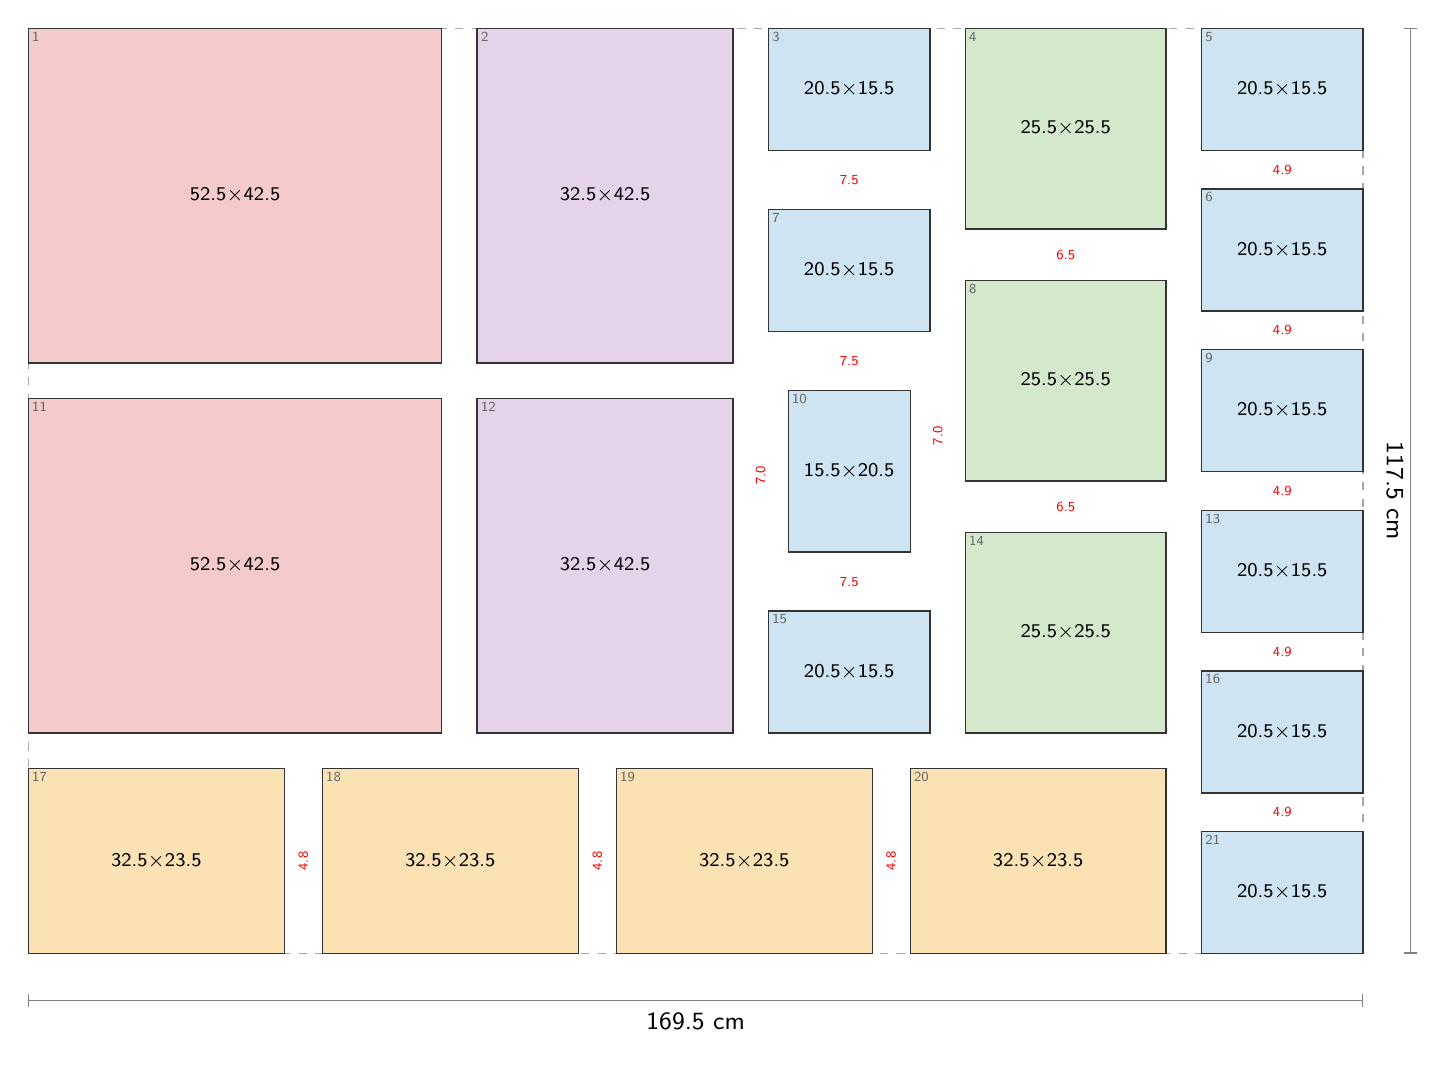
\begin{tikzpicture}[x=1mm, y=-1mm]
\draw[gray!70, dashed, line width=0.4pt] (0,0) rectangle (169.50,117.50);
\filldraw[fill=ft4, draw=black!80, line width=0.5pt] (0.00,0.00) rectangle (52.50,42.50);
\node[align=center, inner sep=0pt] at (26.25,21.25) {\scriptsize 52.5$\times$42.5};
\node[anchor=north west, inner sep=1.2pt, font=\tiny, text=black!60] at (0.00,0.00) {1};
\filldraw[fill=ft3, draw=black!80, line width=0.5pt] (57.00,0.00) rectangle (89.50,42.50);
\node[align=center, inner sep=0pt] at (73.25,21.25) {\scriptsize 32.5$\times$42.5};
\node[anchor=north west, inner sep=1.2pt, font=\tiny, text=black!60] at (57.00,0.00) {2};
\filldraw[fill=ft0, draw=black!80, line width=0.5pt] (94.00,0.00) rectangle (114.50,15.50);
\node[align=center, inner sep=0pt] at (104.25,7.75) {\scriptsize 20.5$\times$15.5};
\node[anchor=north west, inner sep=1.2pt, font=\tiny, text=black!60] at (94.00,0.00) {3};
\filldraw[fill=ft2, draw=black!80, line width=0.5pt] (119.00,0.00) rectangle (144.50,25.50);
\node[align=center, inner sep=0pt] at (131.75,12.75) {\scriptsize 25.5$\times$25.5};
\node[anchor=north west, inner sep=1.2pt, font=\tiny, text=black!60] at (119.00,0.00) {4};
\filldraw[fill=ft0, draw=black!80, line width=0.5pt] (149.00,0.00) rectangle (169.50,15.50);
\node[align=center, inner sep=0pt] at (159.25,7.75) {\scriptsize 20.5$\times$15.5};
\node[anchor=north west, inner sep=1.2pt, font=\tiny, text=black!60] at (149.00,0.00) {5};
\filldraw[fill=ft0, draw=black!80, line width=0.5pt] (149.00,20.40) rectangle (169.50,35.90);
\node[align=center, inner sep=0pt] at (159.25,28.15) {\scriptsize 20.5$\times$15.5};
\node[anchor=north west, inner sep=1.2pt, font=\tiny, text=black!60] at (149.00,20.40) {6};
\filldraw[fill=ft0, draw=black!80, line width=0.5pt] (94.00,23.00) rectangle (114.50,38.50);
\node[align=center, inner sep=0pt] at (104.25,30.75) {\scriptsize 20.5$\times$15.5};
\node[anchor=north west, inner sep=1.2pt, font=\tiny, text=black!60] at (94.00,23.00) {7};
\filldraw[fill=ft2, draw=black!80, line width=0.5pt] (119.00,32.00) rectangle (144.50,57.50);
\node[align=center, inner sep=0pt] at (131.75,44.75) {\scriptsize 25.5$\times$25.5};
\node[anchor=north west, inner sep=1.2pt, font=\tiny, text=black!60] at (119.00,32.00) {8};
\filldraw[fill=ft0, draw=black!80, line width=0.5pt] (149.00,40.80) rectangle (169.50,56.30);
\node[align=center, inner sep=0pt] at (159.25,48.55) {\scriptsize 20.5$\times$15.5};
\node[anchor=north west, inner sep=1.2pt, font=\tiny, text=black!60] at (149.00,40.80) {9};
\filldraw[fill=ft0, draw=black!80, line width=0.5pt] (96.50,46.00) rectangle (112.00,66.50);
\node[align=center, inner sep=0pt] at (104.25,56.25) {\scriptsize 15.5$\times$20.5};
\node[anchor=north west, inner sep=1.2pt, font=\tiny, text=black!60] at (96.50,46.00) {10};
\filldraw[fill=ft4, draw=black!80, line width=0.5pt] (0.00,47.00) rectangle (52.50,89.50);
\node[align=center, inner sep=0pt] at (26.25,68.25) {\scriptsize 52.5$\times$42.5};
\node[anchor=north west, inner sep=1.2pt, font=\tiny, text=black!60] at (0.00,47.00) {11};
\filldraw[fill=ft3, draw=black!80, line width=0.5pt] (57.00,47.00) rectangle (89.50,89.50);
\node[align=center, inner sep=0pt] at (73.25,68.25) {\scriptsize 32.5$\times$42.5};
\node[anchor=north west, inner sep=1.2pt, font=\tiny, text=black!60] at (57.00,47.00) {12};
\filldraw[fill=ft0, draw=black!80, line width=0.5pt] (149.00,61.20) rectangle (169.50,76.70);
\node[align=center, inner sep=0pt] at (159.25,68.95) {\scriptsize 20.5$\times$15.5};
\node[anchor=north west, inner sep=1.2pt, font=\tiny, text=black!60] at (149.00,61.20) {13};
\filldraw[fill=ft2, draw=black!80, line width=0.5pt] (119.00,64.00) rectangle (144.50,89.50);
\node[align=center, inner sep=0pt] at (131.75,76.75) {\scriptsize 25.5$\times$25.5};
\node[anchor=north west, inner sep=1.2pt, font=\tiny, text=black!60] at (119.00,64.00) {14};
\filldraw[fill=ft0, draw=black!80, line width=0.5pt] (94.00,74.00) rectangle (114.50,89.50);
\node[align=center, inner sep=0pt] at (104.25,81.75) {\scriptsize 20.5$\times$15.5};
\node[anchor=north west, inner sep=1.2pt, font=\tiny, text=black!60] at (94.00,74.00) {15};
\filldraw[fill=ft0, draw=black!80, line width=0.5pt] (149.00,81.60) rectangle (169.50,97.10);
\node[align=center, inner sep=0pt] at (159.25,89.35) {\scriptsize 20.5$\times$15.5};
\node[anchor=north west, inner sep=1.2pt, font=\tiny, text=black!60] at (149.00,81.60) {16};
\filldraw[fill=ft1, draw=black!80, line width=0.5pt] (0.00,94.00) rectangle (32.50,117.50);
\node[align=center, inner sep=0pt] at (16.25,105.75) {\scriptsize 32.5$\times$23.5};
\node[anchor=north west, inner sep=1.2pt, font=\tiny, text=black!60] at (0.00,94.00) {17};
\filldraw[fill=ft1, draw=black!80, line width=0.5pt] (37.33,94.00) rectangle (69.83,117.50);
\node[align=center, inner sep=0pt] at (53.58,105.75) {\scriptsize 32.5$\times$23.5};
\node[anchor=north west, inner sep=1.2pt, font=\tiny, text=black!60] at (37.33,94.00) {18};
\filldraw[fill=ft1, draw=black!80, line width=0.5pt] (74.67,94.00) rectangle (107.17,117.50);
\node[align=center, inner sep=0pt] at (90.92,105.75) {\scriptsize 32.5$\times$23.5};
\node[anchor=north west, inner sep=1.2pt, font=\tiny, text=black!60] at (74.67,94.00) {19};
\filldraw[fill=ft1, draw=black!80, line width=0.5pt] (112.00,94.00) rectangle (144.50,117.50);
\node[align=center, inner sep=0pt] at (128.25,105.75) {\scriptsize 32.5$\times$23.5};
\node[anchor=north west, inner sep=1.2pt, font=\tiny, text=black!60] at (112.00,94.00) {20};
\filldraw[fill=ft0, draw=black!80, line width=0.5pt] (149.00,102.00) rectangle (169.50,117.50);
\node[align=center, inner sep=0pt] at (159.25,109.75) {\scriptsize 20.5$\times$15.5};
\node[anchor=north west, inner sep=1.2pt, font=\tiny, text=black!60] at (149.00,102.00) {21};
\node[font=\tiny, text=red, fill=white, inner sep=0.3pt] at (104.25,19.25) {7.5};
\node[font=\tiny, text=red, fill=white, inner sep=0.3pt] at (131.75,28.75) {6.5};
\node[font=\tiny, text=red, fill=white, inner sep=0.3pt] at (159.25,17.95) {4.9};
\node[font=\tiny, text=red, fill=white, inner sep=0.3pt] at (159.25,38.35) {4.9};
\node[font=\tiny, text=red, fill=white, inner sep=0.3pt] at (104.25,42.25) {7.5};
\node[font=\tiny, text=red, fill=white, inner sep=0.3pt] at (131.75,60.75) {6.5};
\node[font=\tiny, text=red, fill=white, inner sep=0.3pt] at (159.25,58.75) {4.9};
\node[font=\tiny, text=red, fill=white, inner sep=0.3pt, rotate=90] at (115.50,51.75) {7.0};
\node[font=\tiny, text=red, fill=white, inner sep=0.3pt] at (104.25,70.25) {7.5};
\node[font=\tiny, text=red, fill=white, inner sep=0.3pt, rotate=90] at (93.00,56.75) {7.0};
\node[font=\tiny, text=red, fill=white, inner sep=0.3pt] at (159.25,79.15) {4.9};
\node[font=\tiny, text=red, fill=white, inner sep=0.3pt] at (159.25,99.55) {4.9};
\node[font=\tiny, text=red, fill=white, inner sep=0.3pt, rotate=90] at (34.92,105.75) {4.8};
\node[font=\tiny, text=red, fill=white, inner sep=0.3pt, rotate=90] at (72.25,105.75) {4.8};
\node[font=\tiny, text=red, fill=white, inner sep=0.3pt, rotate=90] at (109.58,105.75) {4.8};
\draw[Bar-Bar, gray] (0,123.50) -- (169.50,123.50) node[midway, below=1pt, font=\small, text=black] {169.5 cm};
\draw[Bar-Bar, gray] (175.50,0) -- (175.50,117.50) node[midway, right=1pt, font=\small, text=black, rotate=-90, anchor=north] {117.5 cm};
\end{tikzpicture}\\[4pt]
{\scriptsize Scale 1:10 (1 mm = 1 cm). Red numbers mark gaps that deviate from the nominal gap by more than 0.25 cm. Small grey numbers index the coordinate table.}
\end{minipage}\hfill
\begin{minipage}[t]{0.25\textwidth}\vspace{0pt}
\small
\begin{tabular}{@{}l l@{}}
\toprule
Outer size & 169.5 $\times$ 117.5 cm \\
Nominal gap & 4.5 cm \\
Actual gaps & 4.5 -- 7.5 cm \\
Max.\ deviation & 3.0 cm \\
Mean deviation & 0.57 cm \\
Border notches & none \\
Corners filled & 4 / 4 \\
Frames used & 21 of 28 \\
\bottomrule
\end{tabular}

\vspace{8pt}
\scriptsize
\begin{tabular}{@{}c l l r r@{}}
\toprule
 & outer w $\times$ h (cm) & & used & have \\
\midrule
\tikz[baseline=-0.6ex]\fill[ft0,draw=black!60] (0,0) rectangle (1.2ex,1.2ex); & 20.5$\times$15.5 & L & 9 & 9 \\
\tikz[baseline=-0.6ex]\fill[ft0,draw=black!60] (0,0) rectangle (1.2ex,1.2ex); & 15.5$\times$20.5 & P & 1 & 2 \\
\tikz[baseline=-0.6ex]\fill[ft3,draw=black!60] (0,0) rectangle (1.2ex,1.2ex); & 32.5$\times$42.5 & P & 2 & 2 \\
\tikz[baseline=-0.6ex]\fill[ft3,draw=black!60] (0,0) rectangle (1.2ex,1.2ex); & 42.5$\times$32.5 & L & 0 & 1 \\
\tikz[baseline=-0.6ex]\fill[ft1,draw=black!60] (0,0) rectangle (1.2ex,1.2ex); & 32.5$\times$23.5 & L & 4 & 5 \\
\tikz[baseline=-0.6ex]\fill[ft1,draw=black!60] (0,0) rectangle (1.2ex,1.2ex); & 23.5$\times$32.5 & P & 0 & 1 \\
\tikz[baseline=-0.6ex]\fill[ft2,draw=black!60] (0,0) rectangle (1.2ex,1.2ex); & 25.5$\times$25.5 &  & 3 & 5 \\
\tikz[baseline=-0.6ex]\fill[ft4,draw=black!60] (0,0) rectangle (1.2ex,1.2ex); & 42.5$\times$52.5 & P & 0 & 1 \\
\tikz[baseline=-0.6ex]\fill[ft4,draw=black!60] (0,0) rectangle (1.2ex,1.2ex); & 52.5$\times$42.5 & L & 2 & 2 \\
\bottomrule
\end{tabular}

\vspace{8pt}
{\bfseries Positions} (top-left corner, cm)\\[2pt]
\tiny
\begin{tabular}{@{}r l r r@{}}
\toprule
\# & frame w $\times$ h & x & y \\
\midrule
1 & 52.5 $\times$ 42.5 & 0.0 & 0.0 \\
2 & 32.5 $\times$ 42.5 & 57.0 & 0.0 \\
3 & 20.5 $\times$ 15.5 & 94.0 & 0.0 \\
4 & 25.5 $\times$ 25.5 & 119.0 & 0.0 \\
5 & 20.5 $\times$ 15.5 & 149.0 & 0.0 \\
6 & 20.5 $\times$ 15.5 & 149.0 & 20.4 \\
7 & 20.5 $\times$ 15.5 & 94.0 & 23.0 \\
8 & 25.5 $\times$ 25.5 & 119.0 & 32.0 \\
9 & 20.5 $\times$ 15.5 & 149.0 & 40.8 \\
10 & 15.5 $\times$ 20.5 & 96.5 & 46.0 \\
11 & 52.5 $\times$ 42.5 & 0.0 & 47.0 \\
12 & 32.5 $\times$ 42.5 & 57.0 & 47.0 \\
13 & 20.5 $\times$ 15.5 & 149.0 & 61.2 \\
14 & 25.5 $\times$ 25.5 & 119.0 & 64.0 \\
15 & 20.5 $\times$ 15.5 & 94.0 & 74.0 \\
16 & 20.5 $\times$ 15.5 & 149.0 & 81.6 \\
17 & 32.5 $\times$ 23.5 & 0.0 & 94.0 \\
18 & 32.5 $\times$ 23.5 & 37.3 & 94.0 \\
19 & 32.5 $\times$ 23.5 & 74.7 & 94.0 \\
20 & 32.5 $\times$ 23.5 & 112.0 & 94.0 \\
21 & 20.5 $\times$ 15.5 & 149.0 & 102.0 \\
\bottomrule
\end{tabular}
\end{minipage}
\clearpage

\begin{minipage}[t]{0.74\textwidth}\vspace{0pt}
{\LARGE\bfseries Layout 5}\hspace{1.5em}{\large 179.5 $\times$ 123.5 cm \quad gap 2 cm \quad 25 frames}\\[8pt]
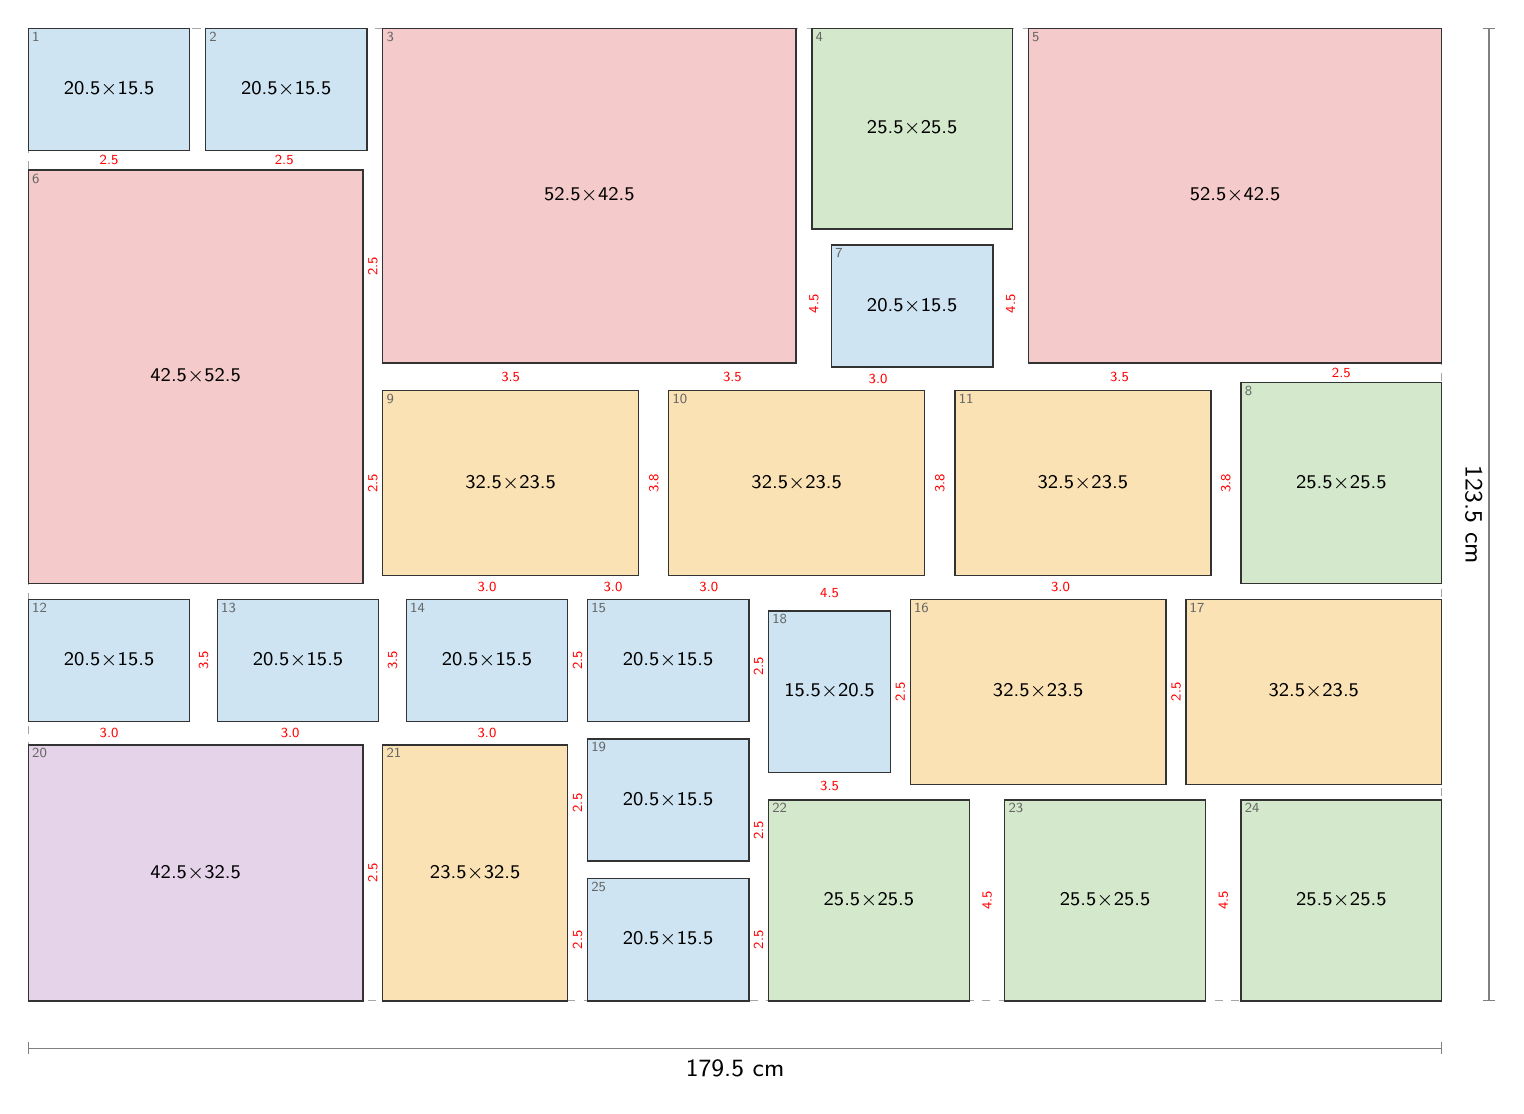
\begin{tikzpicture}[x=1mm, y=-1mm]
\draw[gray!70, dashed, line width=0.4pt] (0,0) rectangle (179.50,123.50);
\filldraw[fill=ft0, draw=black!80, line width=0.5pt] (0.00,0.00) rectangle (20.50,15.50);
\node[align=center, inner sep=0pt] at (10.25,7.75) {\scriptsize 20.5$\times$15.5};
\node[anchor=north west, inner sep=1.2pt, font=\tiny, text=black!60] at (0.00,0.00) {1};
\filldraw[fill=ft0, draw=black!80, line width=0.5pt] (22.50,0.00) rectangle (43.00,15.50);
\node[align=center, inner sep=0pt] at (32.75,7.75) {\scriptsize 20.5$\times$15.5};
\node[anchor=north west, inner sep=1.2pt, font=\tiny, text=black!60] at (22.50,0.00) {2};
\filldraw[fill=ft4, draw=black!80, line width=0.5pt] (45.00,0.00) rectangle (97.50,42.50);
\node[align=center, inner sep=0pt] at (71.25,21.25) {\scriptsize 52.5$\times$42.5};
\node[anchor=north west, inner sep=1.2pt, font=\tiny, text=black!60] at (45.00,0.00) {3};
\filldraw[fill=ft2, draw=black!80, line width=0.5pt] (99.50,0.00) rectangle (125.00,25.50);
\node[align=center, inner sep=0pt] at (112.25,12.75) {\scriptsize 25.5$\times$25.5};
\node[anchor=north west, inner sep=1.2pt, font=\tiny, text=black!60] at (99.50,0.00) {4};
\filldraw[fill=ft4, draw=black!80, line width=0.5pt] (127.00,0.00) rectangle (179.50,42.50);
\node[align=center, inner sep=0pt] at (153.25,21.25) {\scriptsize 52.5$\times$42.5};
\node[anchor=north west, inner sep=1.2pt, font=\tiny, text=black!60] at (127.00,0.00) {5};
\filldraw[fill=ft4, draw=black!80, line width=0.5pt] (0.00,18.00) rectangle (42.50,70.50);
\node[align=center, inner sep=0pt] at (21.25,44.25) {\scriptsize 42.5$\times$52.5};
\node[anchor=north west, inner sep=1.2pt, font=\tiny, text=black!60] at (0.00,18.00) {6};
\filldraw[fill=ft0, draw=black!80, line width=0.5pt] (102.00,27.50) rectangle (122.50,43.00);
\node[align=center, inner sep=0pt] at (112.25,35.25) {\scriptsize 20.5$\times$15.5};
\node[anchor=north west, inner sep=1.2pt, font=\tiny, text=black!60] at (102.00,27.50) {7};
\filldraw[fill=ft2, draw=black!80, line width=0.5pt] (154.00,45.00) rectangle (179.50,70.50);
\node[align=center, inner sep=0pt] at (166.75,57.75) {\scriptsize 25.5$\times$25.5};
\node[anchor=north west, inner sep=1.2pt, font=\tiny, text=black!60] at (154.00,45.00) {8};
\filldraw[fill=ft1, draw=black!80, line width=0.5pt] (45.00,46.00) rectangle (77.50,69.50);
\node[align=center, inner sep=0pt] at (61.25,57.75) {\scriptsize 32.5$\times$23.5};
\node[anchor=north west, inner sep=1.2pt, font=\tiny, text=black!60] at (45.00,46.00) {9};
\filldraw[fill=ft1, draw=black!80, line width=0.5pt] (81.33,46.00) rectangle (113.83,69.50);
\node[align=center, inner sep=0pt] at (97.58,57.75) {\scriptsize 32.5$\times$23.5};
\node[anchor=north west, inner sep=1.2pt, font=\tiny, text=black!60] at (81.33,46.00) {10};
\filldraw[fill=ft1, draw=black!80, line width=0.5pt] (117.67,46.00) rectangle (150.17,69.50);
\node[align=center, inner sep=0pt] at (133.92,57.75) {\scriptsize 32.5$\times$23.5};
\node[anchor=north west, inner sep=1.2pt, font=\tiny, text=black!60] at (117.67,46.00) {11};
\filldraw[fill=ft0, draw=black!80, line width=0.5pt] (0.00,72.50) rectangle (20.50,88.00);
\node[align=center, inner sep=0pt] at (10.25,80.25) {\scriptsize 20.5$\times$15.5};
\node[anchor=north west, inner sep=1.2pt, font=\tiny, text=black!60] at (0.00,72.50) {12};
\filldraw[fill=ft0, draw=black!80, line width=0.5pt] (24.00,72.50) rectangle (44.50,88.00);
\node[align=center, inner sep=0pt] at (34.25,80.25) {\scriptsize 20.5$\times$15.5};
\node[anchor=north west, inner sep=1.2pt, font=\tiny, text=black!60] at (24.00,72.50) {13};
\filldraw[fill=ft0, draw=black!80, line width=0.5pt] (48.00,72.50) rectangle (68.50,88.00);
\node[align=center, inner sep=0pt] at (58.25,80.25) {\scriptsize 20.5$\times$15.5};
\node[anchor=north west, inner sep=1.2pt, font=\tiny, text=black!60] at (48.00,72.50) {14};
\filldraw[fill=ft0, draw=black!80, line width=0.5pt] (71.00,72.50) rectangle (91.50,88.00);
\node[align=center, inner sep=0pt] at (81.25,80.25) {\scriptsize 20.5$\times$15.5};
\node[anchor=north west, inner sep=1.2pt, font=\tiny, text=black!60] at (71.00,72.50) {15};
\filldraw[fill=ft1, draw=black!80, line width=0.5pt] (112.00,72.50) rectangle (144.50,96.00);
\node[align=center, inner sep=0pt] at (128.25,84.25) {\scriptsize 32.5$\times$23.5};
\node[anchor=north west, inner sep=1.2pt, font=\tiny, text=black!60] at (112.00,72.50) {16};
\filldraw[fill=ft1, draw=black!80, line width=0.5pt] (147.00,72.50) rectangle (179.50,96.00);
\node[align=center, inner sep=0pt] at (163.25,84.25) {\scriptsize 32.5$\times$23.5};
\node[anchor=north west, inner sep=1.2pt, font=\tiny, text=black!60] at (147.00,72.50) {17};
\filldraw[fill=ft0, draw=black!80, line width=0.5pt] (94.00,74.00) rectangle (109.50,94.50);
\node[align=center, inner sep=0pt] at (101.75,84.25) {\scriptsize 15.5$\times$20.5};
\node[anchor=north west, inner sep=1.2pt, font=\tiny, text=black!60] at (94.00,74.00) {18};
\filldraw[fill=ft0, draw=black!80, line width=0.5pt] (71.00,90.25) rectangle (91.50,105.75);
\node[align=center, inner sep=0pt] at (81.25,98.00) {\scriptsize 20.5$\times$15.5};
\node[anchor=north west, inner sep=1.2pt, font=\tiny, text=black!60] at (71.00,90.25) {19};
\filldraw[fill=ft3, draw=black!80, line width=0.5pt] (0.00,91.00) rectangle (42.50,123.50);
\node[align=center, inner sep=0pt] at (21.25,107.25) {\scriptsize 42.5$\times$32.5};
\node[anchor=north west, inner sep=1.2pt, font=\tiny, text=black!60] at (0.00,91.00) {20};
\filldraw[fill=ft1, draw=black!80, line width=0.5pt] (45.00,91.00) rectangle (68.50,123.50);
\node[align=center, inner sep=0pt] at (56.75,107.25) {\scriptsize 23.5$\times$32.5};
\node[anchor=north west, inner sep=1.2pt, font=\tiny, text=black!60] at (45.00,91.00) {21};
\filldraw[fill=ft2, draw=black!80, line width=0.5pt] (94.00,98.00) rectangle (119.50,123.50);
\node[align=center, inner sep=0pt] at (106.75,110.75) {\scriptsize 25.5$\times$25.5};
\node[anchor=north west, inner sep=1.2pt, font=\tiny, text=black!60] at (94.00,98.00) {22};
\filldraw[fill=ft2, draw=black!80, line width=0.5pt] (124.00,98.00) rectangle (149.50,123.50);
\node[align=center, inner sep=0pt] at (136.75,110.75) {\scriptsize 25.5$\times$25.5};
\node[anchor=north west, inner sep=1.2pt, font=\tiny, text=black!60] at (124.00,98.00) {23};
\filldraw[fill=ft2, draw=black!80, line width=0.5pt] (154.00,98.00) rectangle (179.50,123.50);
\node[align=center, inner sep=0pt] at (166.75,110.75) {\scriptsize 25.5$\times$25.5};
\node[anchor=north west, inner sep=1.2pt, font=\tiny, text=black!60] at (154.00,98.00) {24};
\filldraw[fill=ft0, draw=black!80, line width=0.5pt] (71.00,108.00) rectangle (91.50,123.50);
\node[align=center, inner sep=0pt] at (81.25,115.75) {\scriptsize 20.5$\times$15.5};
\node[anchor=north west, inner sep=1.2pt, font=\tiny, text=black!60] at (71.00,108.00) {25};
\node[font=\tiny, text=red, fill=white, inner sep=0.3pt] at (10.25,16.75) {2.5};
\node[font=\tiny, text=red, fill=white, inner sep=0.3pt] at (32.50,16.75) {2.5};
\node[font=\tiny, text=red, fill=white, inner sep=0.3pt, rotate=90] at (99.75,35.00) {4.5};
\node[font=\tiny, text=red, fill=white, inner sep=0.3pt] at (61.25,44.25) {3.5};
\node[font=\tiny, text=red, fill=white, inner sep=0.3pt] at (89.42,44.25) {3.5};
\node[font=\tiny, text=red, fill=white, inner sep=0.3pt] at (166.75,43.75) {2.5};
\node[font=\tiny, text=red, fill=white, inner sep=0.3pt] at (138.58,44.25) {3.5};
\node[font=\tiny, text=red, fill=white, inner sep=0.3pt, rotate=90] at (43.75,30.25) {2.5};
\node[font=\tiny, text=red, fill=white, inner sep=0.3pt, rotate=90] at (43.75,57.75) {2.5};
\node[font=\tiny, text=red, fill=white, inner sep=0.3pt, rotate=90] at (124.75,35.00) {4.5};
\node[font=\tiny, text=red, fill=white, inner sep=0.3pt] at (107.92,44.50) {3.0};
\node[font=\tiny, text=red, fill=white, inner sep=0.3pt, rotate=90] at (79.42,57.75) {3.8};
\node[font=\tiny, text=red, fill=white, inner sep=0.3pt] at (58.25,71.00) {3.0};
\node[font=\tiny, text=red, fill=white, inner sep=0.3pt] at (74.25,71.00) {3.0};
\node[font=\tiny, text=red, fill=white, inner sep=0.3pt, rotate=90] at (115.75,57.75) {3.8};
\node[font=\tiny, text=red, fill=white, inner sep=0.3pt] at (86.42,71.00) {3.0};
\node[font=\tiny, text=red, fill=white, inner sep=0.3pt] at (101.75,71.75) {4.5};
\node[font=\tiny, text=red, fill=white, inner sep=0.3pt, rotate=90] at (152.08,57.75) {3.8};
\node[font=\tiny, text=red, fill=white, inner sep=0.3pt] at (131.08,71.00) {3.0};
\node[font=\tiny, text=red, fill=white, inner sep=0.3pt, rotate=90] at (22.25,80.25) {3.5};
\node[font=\tiny, text=red, fill=white, inner sep=0.3pt] at (10.25,89.50) {3.0};
\node[font=\tiny, text=red, fill=white, inner sep=0.3pt, rotate=90] at (46.25,80.25) {3.5};
\node[font=\tiny, text=red, fill=white, inner sep=0.3pt] at (33.25,89.50) {3.0};
\node[font=\tiny, text=red, fill=white, inner sep=0.3pt, rotate=90] at (69.75,80.25) {2.5};
\node[font=\tiny, text=red, fill=white, inner sep=0.3pt] at (58.25,89.50) {3.0};
\node[font=\tiny, text=red, fill=white, inner sep=0.3pt, rotate=90] at (92.75,81.00) {2.5};
\node[font=\tiny, text=red, fill=white, inner sep=0.3pt, rotate=90] at (145.75,84.25) {2.5};
\node[font=\tiny, text=red, fill=white, inner sep=0.3pt, rotate=90] at (110.75,84.25) {2.5};
\node[font=\tiny, text=red, fill=white, inner sep=0.3pt] at (101.75,96.25) {3.5};
\node[font=\tiny, text=red, fill=white, inner sep=0.3pt, rotate=90] at (92.75,101.88) {2.5};
\node[font=\tiny, text=red, fill=white, inner sep=0.3pt, rotate=90] at (43.75,107.25) {2.5};
\node[font=\tiny, text=red, fill=white, inner sep=0.3pt, rotate=90] at (69.75,98.38) {2.5};
\node[font=\tiny, text=red, fill=white, inner sep=0.3pt, rotate=90] at (69.75,115.75) {2.5};
\node[font=\tiny, text=red, fill=white, inner sep=0.3pt, rotate=90] at (121.75,110.75) {4.5};
\node[font=\tiny, text=red, fill=white, inner sep=0.3pt, rotate=90] at (151.75,110.75) {4.5};
\node[font=\tiny, text=red, fill=white, inner sep=0.3pt, rotate=90] at (92.75,115.75) {2.5};
\draw[Bar-Bar, gray] (0,129.50) -- (179.50,129.50) node[midway, below=1pt, font=\small, text=black] {179.5 cm};
\draw[Bar-Bar, gray] (185.50,0) -- (185.50,123.50) node[midway, right=1pt, font=\small, text=black, rotate=-90, anchor=north] {123.5 cm};
\end{tikzpicture}\\[4pt]
{\scriptsize Scale 1:10 (1 mm = 1 cm). Red numbers mark gaps that deviate from the nominal gap by more than 0.25 cm. Small grey numbers index the coordinate table.}
\end{minipage}\hfill
\begin{minipage}[t]{0.25\textwidth}\vspace{0pt}
\small
\begin{tabular}{@{}l l@{}}
\toprule
Outer size & 179.5 $\times$ 123.5 cm \\
Nominal gap & 2 cm \\
Actual gaps & 2.0 -- 4.5 cm \\
Max.\ deviation & 2.5 cm \\
Mean deviation & 0.87 cm \\
Border notches & bottom 9 cm \\
Corners filled & 4 / 4 \\
Frames used & 25 of 28 \\
\bottomrule
\end{tabular}

\vspace{8pt}
\scriptsize
\begin{tabular}{@{}c l l r r@{}}
\toprule
 & outer w $\times$ h (cm) & & used & have \\
\midrule
\tikz[baseline=-0.6ex]\fill[ft0,draw=black!60] (0,0) rectangle (1.2ex,1.2ex); & 20.5$\times$15.5 & L & 9 & 9 \\
\tikz[baseline=-0.6ex]\fill[ft0,draw=black!60] (0,0) rectangle (1.2ex,1.2ex); & 15.5$\times$20.5 & P & 1 & 2 \\
\tikz[baseline=-0.6ex]\fill[ft3,draw=black!60] (0,0) rectangle (1.2ex,1.2ex); & 32.5$\times$42.5 & P & 0 & 2 \\
\tikz[baseline=-0.6ex]\fill[ft3,draw=black!60] (0,0) rectangle (1.2ex,1.2ex); & 42.5$\times$32.5 & L & 1 & 1 \\
\tikz[baseline=-0.6ex]\fill[ft1,draw=black!60] (0,0) rectangle (1.2ex,1.2ex); & 32.5$\times$23.5 & L & 5 & 5 \\
\tikz[baseline=-0.6ex]\fill[ft1,draw=black!60] (0,0) rectangle (1.2ex,1.2ex); & 23.5$\times$32.5 & P & 1 & 1 \\
\tikz[baseline=-0.6ex]\fill[ft2,draw=black!60] (0,0) rectangle (1.2ex,1.2ex); & 25.5$\times$25.5 &  & 5 & 5 \\
\tikz[baseline=-0.6ex]\fill[ft4,draw=black!60] (0,0) rectangle (1.2ex,1.2ex); & 42.5$\times$52.5 & P & 1 & 1 \\
\tikz[baseline=-0.6ex]\fill[ft4,draw=black!60] (0,0) rectangle (1.2ex,1.2ex); & 52.5$\times$42.5 & L & 2 & 2 \\
\bottomrule
\end{tabular}

\vspace{8pt}
{\bfseries Positions} (top-left corner, cm)\\[2pt]
\tiny
\begin{tabular}{@{}r l r r@{}}
\toprule
\# & frame w $\times$ h & x & y \\
\midrule
1 & 20.5 $\times$ 15.5 & 0.0 & 0.0 \\
2 & 20.5 $\times$ 15.5 & 22.5 & 0.0 \\
3 & 52.5 $\times$ 42.5 & 45.0 & 0.0 \\
4 & 25.5 $\times$ 25.5 & 99.5 & 0.0 \\
5 & 52.5 $\times$ 42.5 & 127.0 & 0.0 \\
6 & 42.5 $\times$ 52.5 & 0.0 & 18.0 \\
7 & 20.5 $\times$ 15.5 & 102.0 & 27.5 \\
8 & 25.5 $\times$ 25.5 & 154.0 & 45.0 \\
9 & 32.5 $\times$ 23.5 & 45.0 & 46.0 \\
10 & 32.5 $\times$ 23.5 & 81.3 & 46.0 \\
11 & 32.5 $\times$ 23.5 & 117.7 & 46.0 \\
12 & 20.5 $\times$ 15.5 & 0.0 & 72.5 \\
13 & 20.5 $\times$ 15.5 & 24.0 & 72.5 \\
14 & 20.5 $\times$ 15.5 & 48.0 & 72.5 \\
15 & 20.5 $\times$ 15.5 & 71.0 & 72.5 \\
16 & 32.5 $\times$ 23.5 & 112.0 & 72.5 \\
17 & 32.5 $\times$ 23.5 & 147.0 & 72.5 \\
18 & 15.5 $\times$ 20.5 & 94.0 & 74.0 \\
19 & 20.5 $\times$ 15.5 & 71.0 & 90.2 \\
20 & 42.5 $\times$ 32.5 & 0.0 & 91.0 \\
21 & 23.5 $\times$ 32.5 & 45.0 & 91.0 \\
22 & 25.5 $\times$ 25.5 & 94.0 & 98.0 \\
23 & 25.5 $\times$ 25.5 & 124.0 & 98.0 \\
24 & 25.5 $\times$ 25.5 & 154.0 & 98.0 \\
25 & 20.5 $\times$ 15.5 & 71.0 & 108.0 \\
\bottomrule
\end{tabular}
\end{minipage}
\clearpage

\begin{minipage}[t]{0.74\textwidth}\vspace{0pt}
{\LARGE\bfseries Layout 6}\hspace{1.5em}{\large 177.5 $\times$ 126.5 cm \quad gap 1.5 cm \quad 24 frames}\\[8pt]
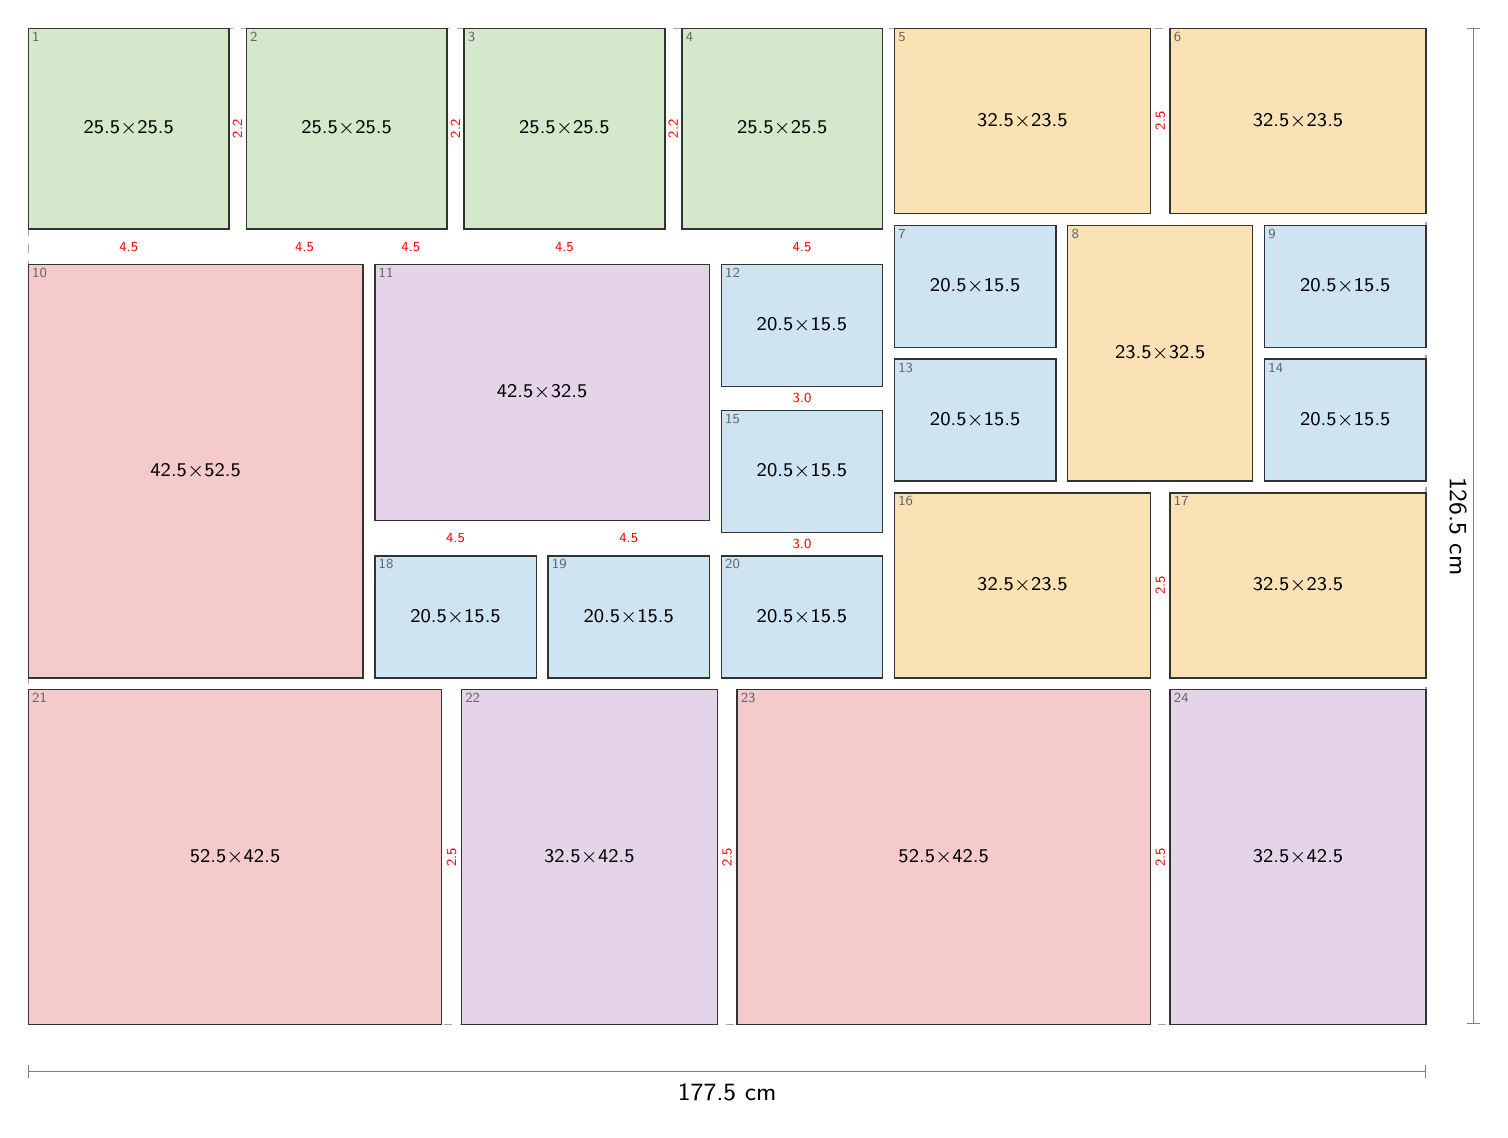
\begin{tikzpicture}[x=1mm, y=-1mm]
\draw[gray!70, dashed, line width=0.4pt] (0,0) rectangle (177.50,126.50);
\filldraw[fill=ft2, draw=black!80, line width=0.5pt] (0.00,0.00) rectangle (25.50,25.50);
\node[align=center, inner sep=0pt] at (12.75,12.75) {\scriptsize 25.5$\times$25.5};
\node[anchor=north west, inner sep=1.2pt, font=\tiny, text=black!60] at (0.00,0.00) {1};
\filldraw[fill=ft2, draw=black!80, line width=0.5pt] (27.67,0.00) rectangle (53.17,25.50);
\node[align=center, inner sep=0pt] at (40.42,12.75) {\scriptsize 25.5$\times$25.5};
\node[anchor=north west, inner sep=1.2pt, font=\tiny, text=black!60] at (27.67,0.00) {2};
\filldraw[fill=ft2, draw=black!80, line width=0.5pt] (55.33,0.00) rectangle (80.83,25.50);
\node[align=center, inner sep=0pt] at (68.08,12.75) {\scriptsize 25.5$\times$25.5};
\node[anchor=north west, inner sep=1.2pt, font=\tiny, text=black!60] at (55.33,0.00) {3};
\filldraw[fill=ft2, draw=black!80, line width=0.5pt] (83.00,0.00) rectangle (108.50,25.50);
\node[align=center, inner sep=0pt] at (95.75,12.75) {\scriptsize 25.5$\times$25.5};
\node[anchor=north west, inner sep=1.2pt, font=\tiny, text=black!60] at (83.00,0.00) {4};
\filldraw[fill=ft1, draw=black!80, line width=0.5pt] (110.00,0.00) rectangle (142.50,23.50);
\node[align=center, inner sep=0pt] at (126.25,11.75) {\scriptsize 32.5$\times$23.5};
\node[anchor=north west, inner sep=1.2pt, font=\tiny, text=black!60] at (110.00,0.00) {5};
\filldraw[fill=ft1, draw=black!80, line width=0.5pt] (145.00,0.00) rectangle (177.50,23.50);
\node[align=center, inner sep=0pt] at (161.25,11.75) {\scriptsize 32.5$\times$23.5};
\node[anchor=north west, inner sep=1.2pt, font=\tiny, text=black!60] at (145.00,0.00) {6};
\filldraw[fill=ft0, draw=black!80, line width=0.5pt] (110.00,25.00) rectangle (130.50,40.50);
\node[align=center, inner sep=0pt] at (120.25,32.75) {\scriptsize 20.5$\times$15.5};
\node[anchor=north west, inner sep=1.2pt, font=\tiny, text=black!60] at (110.00,25.00) {7};
\filldraw[fill=ft1, draw=black!80, line width=0.5pt] (132.00,25.00) rectangle (155.50,57.50);
\node[align=center, inner sep=0pt] at (143.75,41.25) {\scriptsize 23.5$\times$32.5};
\node[anchor=north west, inner sep=1.2pt, font=\tiny, text=black!60] at (132.00,25.00) {8};
\filldraw[fill=ft0, draw=black!80, line width=0.5pt] (157.00,25.00) rectangle (177.50,40.50);
\node[align=center, inner sep=0pt] at (167.25,32.75) {\scriptsize 20.5$\times$15.5};
\node[anchor=north west, inner sep=1.2pt, font=\tiny, text=black!60] at (157.00,25.00) {9};
\filldraw[fill=ft4, draw=black!80, line width=0.5pt] (0.00,30.00) rectangle (42.50,82.50);
\node[align=center, inner sep=0pt] at (21.25,56.25) {\scriptsize 42.5$\times$52.5};
\node[anchor=north west, inner sep=1.2pt, font=\tiny, text=black!60] at (0.00,30.00) {10};
\filldraw[fill=ft3, draw=black!80, line width=0.5pt] (44.00,30.00) rectangle (86.50,62.50);
\node[align=center, inner sep=0pt] at (65.25,46.25) {\scriptsize 42.5$\times$32.5};
\node[anchor=north west, inner sep=1.2pt, font=\tiny, text=black!60] at (44.00,30.00) {11};
\filldraw[fill=ft0, draw=black!80, line width=0.5pt] (88.00,30.00) rectangle (108.50,45.50);
\node[align=center, inner sep=0pt] at (98.25,37.75) {\scriptsize 20.5$\times$15.5};
\node[anchor=north west, inner sep=1.2pt, font=\tiny, text=black!60] at (88.00,30.00) {12};
\filldraw[fill=ft0, draw=black!80, line width=0.5pt] (110.00,42.00) rectangle (130.50,57.50);
\node[align=center, inner sep=0pt] at (120.25,49.75) {\scriptsize 20.5$\times$15.5};
\node[anchor=north west, inner sep=1.2pt, font=\tiny, text=black!60] at (110.00,42.00) {13};
\filldraw[fill=ft0, draw=black!80, line width=0.5pt] (157.00,42.00) rectangle (177.50,57.50);
\node[align=center, inner sep=0pt] at (167.25,49.75) {\scriptsize 20.5$\times$15.5};
\node[anchor=north west, inner sep=1.2pt, font=\tiny, text=black!60] at (157.00,42.00) {14};
\filldraw[fill=ft0, draw=black!80, line width=0.5pt] (88.00,48.50) rectangle (108.50,64.00);
\node[align=center, inner sep=0pt] at (98.25,56.25) {\scriptsize 20.5$\times$15.5};
\node[anchor=north west, inner sep=1.2pt, font=\tiny, text=black!60] at (88.00,48.50) {15};
\filldraw[fill=ft1, draw=black!80, line width=0.5pt] (110.00,59.00) rectangle (142.50,82.50);
\node[align=center, inner sep=0pt] at (126.25,70.75) {\scriptsize 32.5$\times$23.5};
\node[anchor=north west, inner sep=1.2pt, font=\tiny, text=black!60] at (110.00,59.00) {16};
\filldraw[fill=ft1, draw=black!80, line width=0.5pt] (145.00,59.00) rectangle (177.50,82.50);
\node[align=center, inner sep=0pt] at (161.25,70.75) {\scriptsize 32.5$\times$23.5};
\node[anchor=north west, inner sep=1.2pt, font=\tiny, text=black!60] at (145.00,59.00) {17};
\filldraw[fill=ft0, draw=black!80, line width=0.5pt] (44.00,67.00) rectangle (64.50,82.50);
\node[align=center, inner sep=0pt] at (54.25,74.75) {\scriptsize 20.5$\times$15.5};
\node[anchor=north west, inner sep=1.2pt, font=\tiny, text=black!60] at (44.00,67.00) {18};
\filldraw[fill=ft0, draw=black!80, line width=0.5pt] (66.00,67.00) rectangle (86.50,82.50);
\node[align=center, inner sep=0pt] at (76.25,74.75) {\scriptsize 20.5$\times$15.5};
\node[anchor=north west, inner sep=1.2pt, font=\tiny, text=black!60] at (66.00,67.00) {19};
\filldraw[fill=ft0, draw=black!80, line width=0.5pt] (88.00,67.00) rectangle (108.50,82.50);
\node[align=center, inner sep=0pt] at (98.25,74.75) {\scriptsize 20.5$\times$15.5};
\node[anchor=north west, inner sep=1.2pt, font=\tiny, text=black!60] at (88.00,67.00) {20};
\filldraw[fill=ft4, draw=black!80, line width=0.5pt] (0.00,84.00) rectangle (52.50,126.50);
\node[align=center, inner sep=0pt] at (26.25,105.25) {\scriptsize 52.5$\times$42.5};
\node[anchor=north west, inner sep=1.2pt, font=\tiny, text=black!60] at (0.00,84.00) {21};
\filldraw[fill=ft3, draw=black!80, line width=0.5pt] (55.00,84.00) rectangle (87.50,126.50);
\node[align=center, inner sep=0pt] at (71.25,105.25) {\scriptsize 32.5$\times$42.5};
\node[anchor=north west, inner sep=1.2pt, font=\tiny, text=black!60] at (55.00,84.00) {22};
\filldraw[fill=ft4, draw=black!80, line width=0.5pt] (90.00,84.00) rectangle (142.50,126.50);
\node[align=center, inner sep=0pt] at (116.25,105.25) {\scriptsize 52.5$\times$42.5};
\node[anchor=north west, inner sep=1.2pt, font=\tiny, text=black!60] at (90.00,84.00) {23};
\filldraw[fill=ft3, draw=black!80, line width=0.5pt] (145.00,84.00) rectangle (177.50,126.50);
\node[align=center, inner sep=0pt] at (161.25,105.25) {\scriptsize 32.5$\times$42.5};
\node[anchor=north west, inner sep=1.2pt, font=\tiny, text=black!60] at (145.00,84.00) {24};
\node[font=\tiny, text=red, fill=white, inner sep=0.3pt, rotate=90] at (26.58,12.75) {2.2};
\node[font=\tiny, text=red, fill=white, inner sep=0.3pt] at (12.75,27.75) {4.5};
\node[font=\tiny, text=red, fill=white, inner sep=0.3pt, rotate=90] at (54.25,12.75) {2.2};
\node[font=\tiny, text=red, fill=white, inner sep=0.3pt] at (35.08,27.75) {4.5};
\node[font=\tiny, text=red, fill=white, inner sep=0.3pt] at (48.58,27.75) {4.5};
\node[font=\tiny, text=red, fill=white, inner sep=0.3pt, rotate=90] at (81.92,12.75) {2.2};
\node[font=\tiny, text=red, fill=white, inner sep=0.3pt] at (68.08,27.75) {4.5};
\node[font=\tiny, text=red, fill=white, inner sep=0.3pt] at (98.25,27.75) {4.5};
\node[font=\tiny, text=red, fill=white, inner sep=0.3pt, rotate=90] at (143.75,11.75) {2.5};
\node[font=\tiny, text=red, fill=white, inner sep=0.3pt] at (54.25,64.75) {4.5};
\node[font=\tiny, text=red, fill=white, inner sep=0.3pt] at (76.25,64.75) {4.5};
\node[font=\tiny, text=red, fill=white, inner sep=0.3pt] at (98.25,47.00) {3.0};
\node[font=\tiny, text=red, fill=white, inner sep=0.3pt] at (98.25,65.50) {3.0};
\node[font=\tiny, text=red, fill=white, inner sep=0.3pt, rotate=90] at (143.75,70.75) {2.5};
\node[font=\tiny, text=red, fill=white, inner sep=0.3pt, rotate=90] at (53.75,105.25) {2.5};
\node[font=\tiny, text=red, fill=white, inner sep=0.3pt, rotate=90] at (88.75,105.25) {2.5};
\node[font=\tiny, text=red, fill=white, inner sep=0.3pt, rotate=90] at (143.75,105.25) {2.5};
\draw[Bar-Bar, gray] (0,132.50) -- (177.50,132.50) node[midway, below=1pt, font=\small, text=black] {177.5 cm};
\draw[Bar-Bar, gray] (183.50,0) -- (183.50,126.50) node[midway, right=1pt, font=\small, text=black, rotate=-90, anchor=north] {126.5 cm};
\end{tikzpicture}\\[4pt]
{\scriptsize Scale 1:10 (1 mm = 1 cm). Red numbers mark gaps that deviate from the nominal gap by more than 0.25 cm. Small grey numbers index the coordinate table.}
\end{minipage}\hfill
\begin{minipage}[t]{0.25\textwidth}\vspace{0pt}
\small
\begin{tabular}{@{}l l@{}}
\toprule
Outer size & 177.5 $\times$ 126.5 cm \\
Nominal gap & 1.5 cm \\
Actual gaps & 1.5 -- 4.5 cm \\
Max.\ deviation & 3.0 cm \\
Mean deviation & 0.63 cm \\
Border notches & left 4 cm \\
Corners filled & 4 / 4 \\
Frames used & 24 of 28 \\
\bottomrule
\end{tabular}

\vspace{8pt}
\scriptsize
\begin{tabular}{@{}c l l r r@{}}
\toprule
 & outer w $\times$ h (cm) & & used & have \\
\midrule
\tikz[baseline=-0.6ex]\fill[ft0,draw=black!60] (0,0) rectangle (1.2ex,1.2ex); & 20.5$\times$15.5 & L & 9 & 9 \\
\tikz[baseline=-0.6ex]\fill[ft0,draw=black!60] (0,0) rectangle (1.2ex,1.2ex); & 15.5$\times$20.5 & P & 0 & 2 \\
\tikz[baseline=-0.6ex]\fill[ft3,draw=black!60] (0,0) rectangle (1.2ex,1.2ex); & 32.5$\times$42.5 & P & 2 & 2 \\
\tikz[baseline=-0.6ex]\fill[ft3,draw=black!60] (0,0) rectangle (1.2ex,1.2ex); & 42.5$\times$32.5 & L & 1 & 1 \\
\tikz[baseline=-0.6ex]\fill[ft1,draw=black!60] (0,0) rectangle (1.2ex,1.2ex); & 32.5$\times$23.5 & L & 4 & 5 \\
\tikz[baseline=-0.6ex]\fill[ft1,draw=black!60] (0,0) rectangle (1.2ex,1.2ex); & 23.5$\times$32.5 & P & 1 & 1 \\
\tikz[baseline=-0.6ex]\fill[ft2,draw=black!60] (0,0) rectangle (1.2ex,1.2ex); & 25.5$\times$25.5 &  & 4 & 5 \\
\tikz[baseline=-0.6ex]\fill[ft4,draw=black!60] (0,0) rectangle (1.2ex,1.2ex); & 42.5$\times$52.5 & P & 1 & 1 \\
\tikz[baseline=-0.6ex]\fill[ft4,draw=black!60] (0,0) rectangle (1.2ex,1.2ex); & 52.5$\times$42.5 & L & 2 & 2 \\
\bottomrule
\end{tabular}

\vspace{8pt}
{\bfseries Positions} (top-left corner, cm)\\[2pt]
\tiny
\begin{tabular}{@{}r l r r@{}}
\toprule
\# & frame w $\times$ h & x & y \\
\midrule
1 & 25.5 $\times$ 25.5 & 0.0 & 0.0 \\
2 & 25.5 $\times$ 25.5 & 27.7 & 0.0 \\
3 & 25.5 $\times$ 25.5 & 55.3 & 0.0 \\
4 & 25.5 $\times$ 25.5 & 83.0 & 0.0 \\
5 & 32.5 $\times$ 23.5 & 110.0 & 0.0 \\
6 & 32.5 $\times$ 23.5 & 145.0 & 0.0 \\
7 & 20.5 $\times$ 15.5 & 110.0 & 25.0 \\
8 & 23.5 $\times$ 32.5 & 132.0 & 25.0 \\
9 & 20.5 $\times$ 15.5 & 157.0 & 25.0 \\
10 & 42.5 $\times$ 52.5 & 0.0 & 30.0 \\
11 & 42.5 $\times$ 32.5 & 44.0 & 30.0 \\
12 & 20.5 $\times$ 15.5 & 88.0 & 30.0 \\
13 & 20.5 $\times$ 15.5 & 110.0 & 42.0 \\
14 & 20.5 $\times$ 15.5 & 157.0 & 42.0 \\
15 & 20.5 $\times$ 15.5 & 88.0 & 48.5 \\
16 & 32.5 $\times$ 23.5 & 110.0 & 59.0 \\
17 & 32.5 $\times$ 23.5 & 145.0 & 59.0 \\
18 & 20.5 $\times$ 15.5 & 44.0 & 67.0 \\
19 & 20.5 $\times$ 15.5 & 66.0 & 67.0 \\
20 & 20.5 $\times$ 15.5 & 88.0 & 67.0 \\
21 & 52.5 $\times$ 42.5 & 0.0 & 84.0 \\
22 & 32.5 $\times$ 42.5 & 55.0 & 84.0 \\
23 & 52.5 $\times$ 42.5 & 90.0 & 84.0 \\
24 & 32.5 $\times$ 42.5 & 145.0 & 84.0 \\
\bottomrule
\end{tabular}
\end{minipage}
\clearpage

\begin{minipage}[t]{0.74\textwidth}\vspace{0pt}
{\LARGE\bfseries Layout 7}\hspace{1.5em}{\large 175.5 $\times$ 123.5 cm \quad gap 2.5 cm \quad 24 frames}\\[8pt]
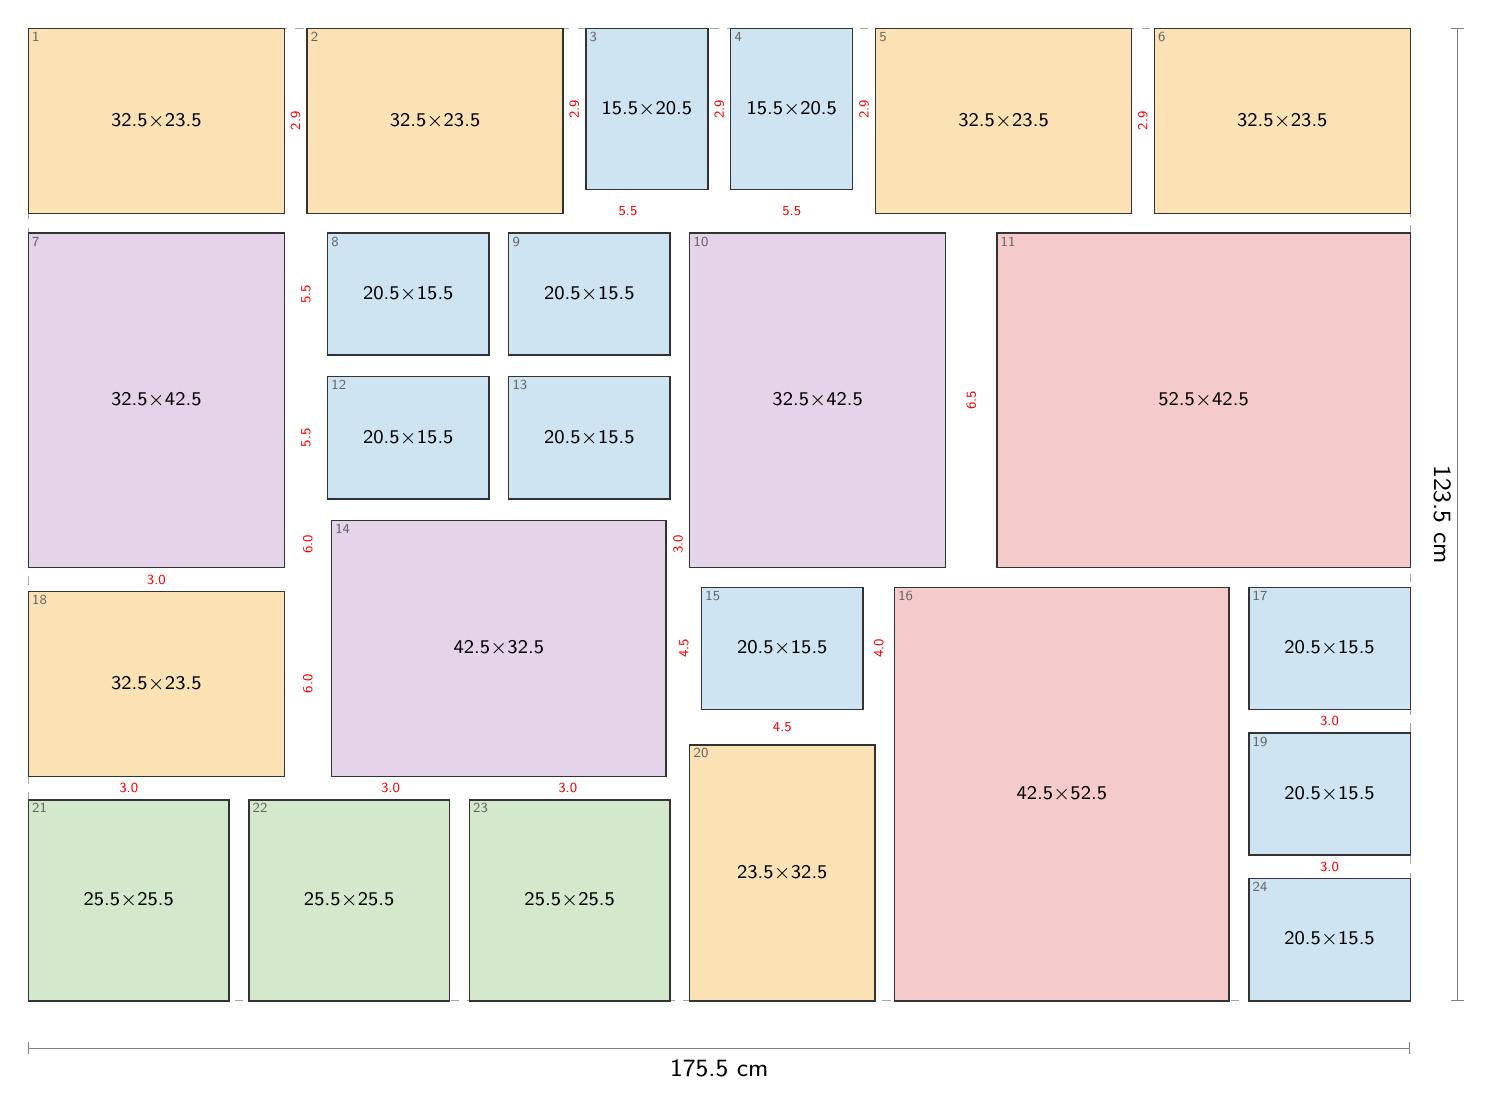
\begin{tikzpicture}[x=1mm, y=-1mm]
\draw[gray!70, dashed, line width=0.4pt] (0,0) rectangle (175.50,123.50);
\filldraw[fill=ft1, draw=black!80, line width=0.5pt] (0.00,0.00) rectangle (32.50,23.50);
\node[align=center, inner sep=0pt] at (16.25,11.75) {\scriptsize 32.5$\times$23.5};
\node[anchor=north west, inner sep=1.2pt, font=\tiny, text=black!60] at (0.00,0.00) {1};
\filldraw[fill=ft1, draw=black!80, line width=0.5pt] (35.40,0.00) rectangle (67.90,23.50);
\node[align=center, inner sep=0pt] at (51.65,11.75) {\scriptsize 32.5$\times$23.5};
\node[anchor=north west, inner sep=1.2pt, font=\tiny, text=black!60] at (35.40,0.00) {2};
\filldraw[fill=ft0, draw=black!80, line width=0.5pt] (70.80,0.00) rectangle (86.30,20.50);
\node[align=center, inner sep=0pt] at (78.55,10.25) {\scriptsize 15.5$\times$20.5};
\node[anchor=north west, inner sep=1.2pt, font=\tiny, text=black!60] at (70.80,0.00) {3};
\filldraw[fill=ft0, draw=black!80, line width=0.5pt] (89.20,0.00) rectangle (104.70,20.50);
\node[align=center, inner sep=0pt] at (96.95,10.25) {\scriptsize 15.5$\times$20.5};
\node[anchor=north west, inner sep=1.2pt, font=\tiny, text=black!60] at (89.20,0.00) {4};
\filldraw[fill=ft1, draw=black!80, line width=0.5pt] (107.60,0.00) rectangle (140.10,23.50);
\node[align=center, inner sep=0pt] at (123.85,11.75) {\scriptsize 32.5$\times$23.5};
\node[anchor=north west, inner sep=1.2pt, font=\tiny, text=black!60] at (107.60,0.00) {5};
\filldraw[fill=ft1, draw=black!80, line width=0.5pt] (143.00,0.00) rectangle (175.50,23.50);
\node[align=center, inner sep=0pt] at (159.25,11.75) {\scriptsize 32.5$\times$23.5};
\node[anchor=north west, inner sep=1.2pt, font=\tiny, text=black!60] at (143.00,0.00) {6};
\filldraw[fill=ft3, draw=black!80, line width=0.5pt] (0.00,26.00) rectangle (32.50,68.50);
\node[align=center, inner sep=0pt] at (16.25,47.25) {\scriptsize 32.5$\times$42.5};
\node[anchor=north west, inner sep=1.2pt, font=\tiny, text=black!60] at (0.00,26.00) {7};
\filldraw[fill=ft0, draw=black!80, line width=0.5pt] (38.00,26.00) rectangle (58.50,41.50);
\node[align=center, inner sep=0pt] at (48.25,33.75) {\scriptsize 20.5$\times$15.5};
\node[anchor=north west, inner sep=1.2pt, font=\tiny, text=black!60] at (38.00,26.00) {8};
\filldraw[fill=ft0, draw=black!80, line width=0.5pt] (61.00,26.00) rectangle (81.50,41.50);
\node[align=center, inner sep=0pt] at (71.25,33.75) {\scriptsize 20.5$\times$15.5};
\node[anchor=north west, inner sep=1.2pt, font=\tiny, text=black!60] at (61.00,26.00) {9};
\filldraw[fill=ft3, draw=black!80, line width=0.5pt] (84.00,26.00) rectangle (116.50,68.50);
\node[align=center, inner sep=0pt] at (100.25,47.25) {\scriptsize 32.5$\times$42.5};
\node[anchor=north west, inner sep=1.2pt, font=\tiny, text=black!60] at (84.00,26.00) {10};
\filldraw[fill=ft4, draw=black!80, line width=0.5pt] (123.00,26.00) rectangle (175.50,68.50);
\node[align=center, inner sep=0pt] at (149.25,47.25) {\scriptsize 52.5$\times$42.5};
\node[anchor=north west, inner sep=1.2pt, font=\tiny, text=black!60] at (123.00,26.00) {11};
\filldraw[fill=ft0, draw=black!80, line width=0.5pt] (38.00,44.25) rectangle (58.50,59.75);
\node[align=center, inner sep=0pt] at (48.25,52.00) {\scriptsize 20.5$\times$15.5};
\node[anchor=north west, inner sep=1.2pt, font=\tiny, text=black!60] at (38.00,44.25) {12};
\filldraw[fill=ft0, draw=black!80, line width=0.5pt] (61.00,44.25) rectangle (81.50,59.75);
\node[align=center, inner sep=0pt] at (71.25,52.00) {\scriptsize 20.5$\times$15.5};
\node[anchor=north west, inner sep=1.2pt, font=\tiny, text=black!60] at (61.00,44.25) {13};
\filldraw[fill=ft3, draw=black!80, line width=0.5pt] (38.50,62.50) rectangle (81.00,95.00);
\node[align=center, inner sep=0pt] at (59.75,78.75) {\scriptsize 42.5$\times$32.5};
\node[anchor=north west, inner sep=1.2pt, font=\tiny, text=black!60] at (38.50,62.50) {14};
\filldraw[fill=ft0, draw=black!80, line width=0.5pt] (85.50,71.00) rectangle (106.00,86.50);
\node[align=center, inner sep=0pt] at (95.75,78.75) {\scriptsize 20.5$\times$15.5};
\node[anchor=north west, inner sep=1.2pt, font=\tiny, text=black!60] at (85.50,71.00) {15};
\filldraw[fill=ft4, draw=black!80, line width=0.5pt] (110.00,71.00) rectangle (152.50,123.50);
\node[align=center, inner sep=0pt] at (131.25,97.25) {\scriptsize 42.5$\times$52.5};
\node[anchor=north west, inner sep=1.2pt, font=\tiny, text=black!60] at (110.00,71.00) {16};
\filldraw[fill=ft0, draw=black!80, line width=0.5pt] (155.00,71.00) rectangle (175.50,86.50);
\node[align=center, inner sep=0pt] at (165.25,78.75) {\scriptsize 20.5$\times$15.5};
\node[anchor=north west, inner sep=1.2pt, font=\tiny, text=black!60] at (155.00,71.00) {17};
\filldraw[fill=ft1, draw=black!80, line width=0.5pt] (0.00,71.50) rectangle (32.50,95.00);
\node[align=center, inner sep=0pt] at (16.25,83.25) {\scriptsize 32.5$\times$23.5};
\node[anchor=north west, inner sep=1.2pt, font=\tiny, text=black!60] at (0.00,71.50) {18};
\filldraw[fill=ft0, draw=black!80, line width=0.5pt] (155.00,89.50) rectangle (175.50,105.00);
\node[align=center, inner sep=0pt] at (165.25,97.25) {\scriptsize 20.5$\times$15.5};
\node[anchor=north west, inner sep=1.2pt, font=\tiny, text=black!60] at (155.00,89.50) {19};
\filldraw[fill=ft1, draw=black!80, line width=0.5pt] (84.00,91.00) rectangle (107.50,123.50);
\node[align=center, inner sep=0pt] at (95.75,107.25) {\scriptsize 23.5$\times$32.5};
\node[anchor=north west, inner sep=1.2pt, font=\tiny, text=black!60] at (84.00,91.00) {20};
\filldraw[fill=ft2, draw=black!80, line width=0.5pt] (0.00,98.00) rectangle (25.50,123.50);
\node[align=center, inner sep=0pt] at (12.75,110.75) {\scriptsize 25.5$\times$25.5};
\node[anchor=north west, inner sep=1.2pt, font=\tiny, text=black!60] at (0.00,98.00) {21};
\filldraw[fill=ft2, draw=black!80, line width=0.5pt] (28.00,98.00) rectangle (53.50,123.50);
\node[align=center, inner sep=0pt] at (40.75,110.75) {\scriptsize 25.5$\times$25.5};
\node[anchor=north west, inner sep=1.2pt, font=\tiny, text=black!60] at (28.00,98.00) {22};
\filldraw[fill=ft2, draw=black!80, line width=0.5pt] (56.00,98.00) rectangle (81.50,123.50);
\node[align=center, inner sep=0pt] at (68.75,110.75) {\scriptsize 25.5$\times$25.5};
\node[anchor=north west, inner sep=1.2pt, font=\tiny, text=black!60] at (56.00,98.00) {23};
\filldraw[fill=ft0, draw=black!80, line width=0.5pt] (155.00,108.00) rectangle (175.50,123.50);
\node[align=center, inner sep=0pt] at (165.25,115.75) {\scriptsize 20.5$\times$15.5};
\node[anchor=north west, inner sep=1.2pt, font=\tiny, text=black!60] at (155.00,108.00) {24};
\node[font=\tiny, text=red, fill=white, inner sep=0.3pt, rotate=90] at (33.95,11.75) {2.9};
\node[font=\tiny, text=red, fill=white, inner sep=0.3pt, rotate=90] at (69.35,10.25) {2.9};
\node[font=\tiny, text=red, fill=white, inner sep=0.3pt, rotate=90] at (87.75,10.25) {2.9};
\node[font=\tiny, text=red, fill=white, inner sep=0.3pt] at (76.15,23.25) {5.5};
\node[font=\tiny, text=red, fill=white, inner sep=0.3pt, rotate=90] at (106.15,10.25) {2.9};
\node[font=\tiny, text=red, fill=white, inner sep=0.3pt] at (96.95,23.25) {5.5};
\node[font=\tiny, text=red, fill=white, inner sep=0.3pt, rotate=90] at (141.55,11.75) {2.9};
\node[font=\tiny, text=red, fill=white, inner sep=0.3pt, rotate=90] at (35.25,33.75) {5.5};
\node[font=\tiny, text=red, fill=white, inner sep=0.3pt, rotate=90] at (35.25,52.00) {5.5};
\node[font=\tiny, text=red, fill=white, inner sep=0.3pt, rotate=90] at (35.50,65.50) {6.0};
\node[font=\tiny, text=red, fill=white, inner sep=0.3pt] at (16.25,70.00) {3.0};
\node[font=\tiny, text=red, fill=white, inner sep=0.3pt, rotate=90] at (119.75,47.25) {6.5};
\node[font=\tiny, text=red, fill=white, inner sep=0.3pt, rotate=90] at (82.50,65.50) {3.0};
\node[font=\tiny, text=red, fill=white, inner sep=0.3pt, rotate=90] at (83.25,78.75) {4.5};
\node[font=\tiny, text=red, fill=white, inner sep=0.3pt] at (46.00,96.50) {3.0};
\node[font=\tiny, text=red, fill=white, inner sep=0.3pt] at (68.50,96.50) {3.0};
\node[font=\tiny, text=red, fill=white, inner sep=0.3pt, rotate=90] at (108.00,78.75) {4.0};
\node[font=\tiny, text=red, fill=white, inner sep=0.3pt] at (95.75,88.75) {4.5};
\node[font=\tiny, text=red, fill=white, inner sep=0.3pt] at (165.25,88.00) {3.0};
\node[font=\tiny, text=red, fill=white, inner sep=0.3pt, rotate=90] at (35.50,83.25) {6.0};
\node[font=\tiny, text=red, fill=white, inner sep=0.3pt] at (12.75,96.50) {3.0};
\node[font=\tiny, text=red, fill=white, inner sep=0.3pt] at (165.25,106.50) {3.0};
\draw[Bar-Bar, gray] (0,129.50) -- (175.50,129.50) node[midway, below=1pt, font=\small, text=black] {175.5 cm};
\draw[Bar-Bar, gray] (181.50,0) -- (181.50,123.50) node[midway, right=1pt, font=\small, text=black, rotate=-90, anchor=north] {123.5 cm};
\end{tikzpicture}\\[4pt]
{\scriptsize Scale 1:10 (1 mm = 1 cm). Red numbers mark gaps that deviate from the nominal gap by more than 0.25 cm. Small grey numbers index the coordinate table.}
\end{minipage}\hfill
\begin{minipage}[t]{0.25\textwidth}\vspace{0pt}
\small
\begin{tabular}{@{}l l@{}}
\toprule
Outer size & 175.5 $\times$ 123.5 cm \\
Nominal gap & 2.5 cm \\
Actual gaps & 2.5 -- 6.5 cm \\
Max.\ deviation & 4.0 cm \\
Mean deviation & 0.74 cm \\
Border notches & none \\
Corners filled & 4 / 4 \\
Frames used & 24 of 28 \\
\bottomrule
\end{tabular}

\vspace{8pt}
\scriptsize
\begin{tabular}{@{}c l l r r@{}}
\toprule
 & outer w $\times$ h (cm) & & used & have \\
\midrule
\tikz[baseline=-0.6ex]\fill[ft0,draw=black!60] (0,0) rectangle (1.2ex,1.2ex); & 20.5$\times$15.5 & L & 8 & 9 \\
\tikz[baseline=-0.6ex]\fill[ft0,draw=black!60] (0,0) rectangle (1.2ex,1.2ex); & 15.5$\times$20.5 & P & 2 & 2 \\
\tikz[baseline=-0.6ex]\fill[ft3,draw=black!60] (0,0) rectangle (1.2ex,1.2ex); & 32.5$\times$42.5 & P & 2 & 2 \\
\tikz[baseline=-0.6ex]\fill[ft3,draw=black!60] (0,0) rectangle (1.2ex,1.2ex); & 42.5$\times$32.5 & L & 1 & 1 \\
\tikz[baseline=-0.6ex]\fill[ft1,draw=black!60] (0,0) rectangle (1.2ex,1.2ex); & 32.5$\times$23.5 & L & 5 & 5 \\
\tikz[baseline=-0.6ex]\fill[ft1,draw=black!60] (0,0) rectangle (1.2ex,1.2ex); & 23.5$\times$32.5 & P & 1 & 1 \\
\tikz[baseline=-0.6ex]\fill[ft2,draw=black!60] (0,0) rectangle (1.2ex,1.2ex); & 25.5$\times$25.5 &  & 3 & 5 \\
\tikz[baseline=-0.6ex]\fill[ft4,draw=black!60] (0,0) rectangle (1.2ex,1.2ex); & 42.5$\times$52.5 & P & 1 & 1 \\
\tikz[baseline=-0.6ex]\fill[ft4,draw=black!60] (0,0) rectangle (1.2ex,1.2ex); & 52.5$\times$42.5 & L & 1 & 2 \\
\bottomrule
\end{tabular}

\vspace{8pt}
{\bfseries Positions} (top-left corner, cm)\\[2pt]
\tiny
\begin{tabular}{@{}r l r r@{}}
\toprule
\# & frame w $\times$ h & x & y \\
\midrule
1 & 32.5 $\times$ 23.5 & 0.0 & 0.0 \\
2 & 32.5 $\times$ 23.5 & 35.4 & 0.0 \\
3 & 15.5 $\times$ 20.5 & 70.8 & 0.0 \\
4 & 15.5 $\times$ 20.5 & 89.2 & 0.0 \\
5 & 32.5 $\times$ 23.5 & 107.6 & 0.0 \\
6 & 32.5 $\times$ 23.5 & 143.0 & 0.0 \\
7 & 32.5 $\times$ 42.5 & 0.0 & 26.0 \\
8 & 20.5 $\times$ 15.5 & 38.0 & 26.0 \\
9 & 20.5 $\times$ 15.5 & 61.0 & 26.0 \\
10 & 32.5 $\times$ 42.5 & 84.0 & 26.0 \\
11 & 52.5 $\times$ 42.5 & 123.0 & 26.0 \\
12 & 20.5 $\times$ 15.5 & 38.0 & 44.2 \\
13 & 20.5 $\times$ 15.5 & 61.0 & 44.2 \\
14 & 42.5 $\times$ 32.5 & 38.5 & 62.5 \\
15 & 20.5 $\times$ 15.5 & 85.5 & 71.0 \\
16 & 42.5 $\times$ 52.5 & 110.0 & 71.0 \\
17 & 20.5 $\times$ 15.5 & 155.0 & 71.0 \\
18 & 32.5 $\times$ 23.5 & 0.0 & 71.5 \\
19 & 20.5 $\times$ 15.5 & 155.0 & 89.5 \\
20 & 23.5 $\times$ 32.5 & 84.0 & 91.0 \\
21 & 25.5 $\times$ 25.5 & 0.0 & 98.0 \\
22 & 25.5 $\times$ 25.5 & 28.0 & 98.0 \\
23 & 25.5 $\times$ 25.5 & 56.0 & 98.0 \\
24 & 20.5 $\times$ 15.5 & 155.0 & 108.0 \\
\bottomrule
\end{tabular}
\end{minipage}
\clearpage

\begin{minipage}[t]{0.74\textwidth}\vspace{0pt}
{\LARGE\bfseries Layout 8}\hspace{1.5em}{\large 189.0 $\times$ 118.0 cm \quad gap 3 cm \quad 23 frames}\\[8pt]
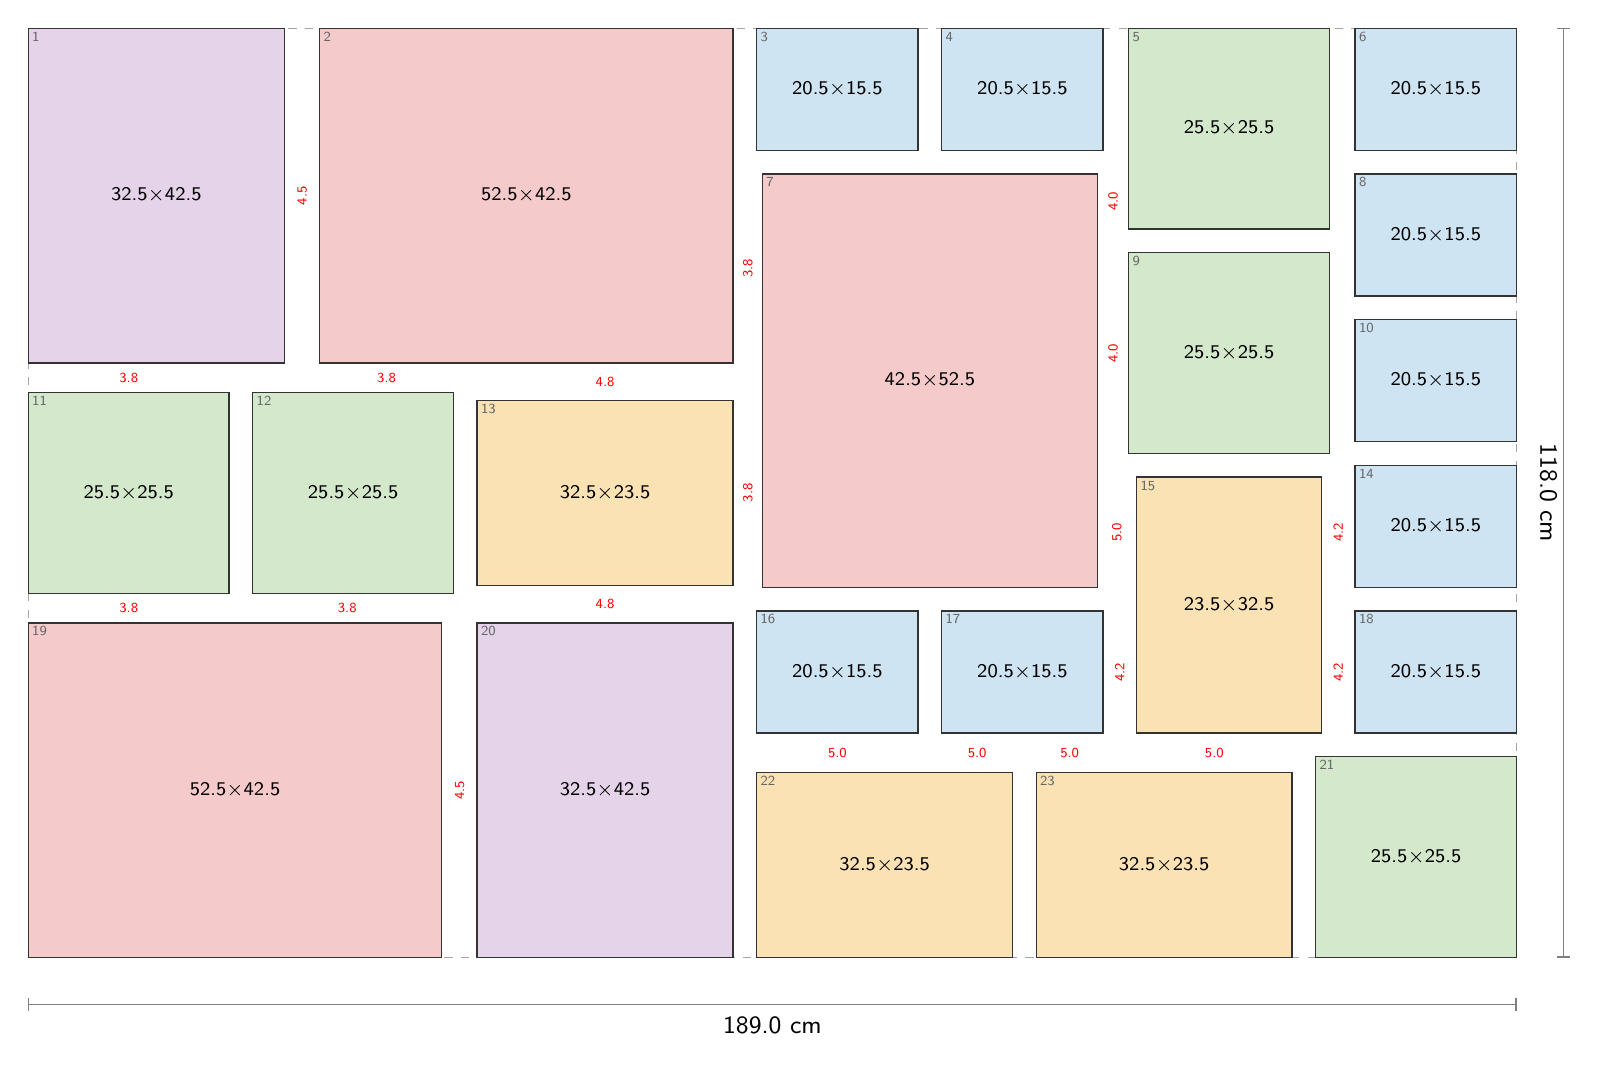
\begin{tikzpicture}[x=1mm, y=-1mm]
\draw[gray!70, dashed, line width=0.4pt] (0,0) rectangle (189.00,118.00);
\filldraw[fill=ft3, draw=black!80, line width=0.5pt] (0.00,0.00) rectangle (32.50,42.50);
\node[align=center, inner sep=0pt] at (16.25,21.25) {\scriptsize 32.5$\times$42.5};
\node[anchor=north west, inner sep=1.2pt, font=\tiny, text=black!60] at (0.00,0.00) {1};
\filldraw[fill=ft4, draw=black!80, line width=0.5pt] (37.00,0.00) rectangle (89.50,42.50);
\node[align=center, inner sep=0pt] at (63.25,21.25) {\scriptsize 52.5$\times$42.5};
\node[anchor=north west, inner sep=1.2pt, font=\tiny, text=black!60] at (37.00,0.00) {2};
\filldraw[fill=ft0, draw=black!80, line width=0.5pt] (92.50,0.00) rectangle (113.00,15.50);
\node[align=center, inner sep=0pt] at (102.75,7.75) {\scriptsize 20.5$\times$15.5};
\node[anchor=north west, inner sep=1.2pt, font=\tiny, text=black!60] at (92.50,0.00) {3};
\filldraw[fill=ft0, draw=black!80, line width=0.5pt] (116.00,0.00) rectangle (136.50,15.50);
\node[align=center, inner sep=0pt] at (126.25,7.75) {\scriptsize 20.5$\times$15.5};
\node[anchor=north west, inner sep=1.2pt, font=\tiny, text=black!60] at (116.00,0.00) {4};
\filldraw[fill=ft2, draw=black!80, line width=0.5pt] (139.75,0.00) rectangle (165.25,25.50);
\node[align=center, inner sep=0pt] at (152.50,12.75) {\scriptsize 25.5$\times$25.5};
\node[anchor=north west, inner sep=1.2pt, font=\tiny, text=black!60] at (139.75,0.00) {5};
\filldraw[fill=ft0, draw=black!80, line width=0.5pt] (168.50,0.00) rectangle (189.00,15.50);
\node[align=center, inner sep=0pt] at (178.75,7.75) {\scriptsize 20.5$\times$15.5};
\node[anchor=north west, inner sep=1.2pt, font=\tiny, text=black!60] at (168.50,0.00) {6};
\filldraw[fill=ft4, draw=black!80, line width=0.5pt] (93.25,18.50) rectangle (135.75,71.00);
\node[align=center, inner sep=0pt] at (114.50,44.75) {\scriptsize 42.5$\times$52.5};
\node[anchor=north west, inner sep=1.2pt, font=\tiny, text=black!60] at (93.25,18.50) {7};
\filldraw[fill=ft0, draw=black!80, line width=0.5pt] (168.50,18.50) rectangle (189.00,34.00);
\node[align=center, inner sep=0pt] at (178.75,26.25) {\scriptsize 20.5$\times$15.5};
\node[anchor=north west, inner sep=1.2pt, font=\tiny, text=black!60] at (168.50,18.50) {8};
\filldraw[fill=ft2, draw=black!80, line width=0.5pt] (139.75,28.50) rectangle (165.25,54.00);
\node[align=center, inner sep=0pt] at (152.50,41.25) {\scriptsize 25.5$\times$25.5};
\node[anchor=north west, inner sep=1.2pt, font=\tiny, text=black!60] at (139.75,28.50) {9};
\filldraw[fill=ft0, draw=black!80, line width=0.5pt] (168.50,37.00) rectangle (189.00,52.50);
\node[align=center, inner sep=0pt] at (178.75,44.75) {\scriptsize 20.5$\times$15.5};
\node[anchor=north west, inner sep=1.2pt, font=\tiny, text=black!60] at (168.50,37.00) {10};
\filldraw[fill=ft2, draw=black!80, line width=0.5pt] (0.00,46.25) rectangle (25.50,71.75);
\node[align=center, inner sep=0pt] at (12.75,59.00) {\scriptsize 25.5$\times$25.5};
\node[anchor=north west, inner sep=1.2pt, font=\tiny, text=black!60] at (0.00,46.25) {11};
\filldraw[fill=ft2, draw=black!80, line width=0.5pt] (28.50,46.25) rectangle (54.00,71.75);
\node[align=center, inner sep=0pt] at (41.25,59.00) {\scriptsize 25.5$\times$25.5};
\node[anchor=north west, inner sep=1.2pt, font=\tiny, text=black!60] at (28.50,46.25) {12};
\filldraw[fill=ft1, draw=black!80, line width=0.5pt] (57.00,47.25) rectangle (89.50,70.75);
\node[align=center, inner sep=0pt] at (73.25,59.00) {\scriptsize 32.5$\times$23.5};
\node[anchor=north west, inner sep=1.2pt, font=\tiny, text=black!60] at (57.00,47.25) {13};
\filldraw[fill=ft0, draw=black!80, line width=0.5pt] (168.50,55.50) rectangle (189.00,71.00);
\node[align=center, inner sep=0pt] at (178.75,63.25) {\scriptsize 20.5$\times$15.5};
\node[anchor=north west, inner sep=1.2pt, font=\tiny, text=black!60] at (168.50,55.50) {14};
\filldraw[fill=ft1, draw=black!80, line width=0.5pt] (140.75,57.00) rectangle (164.25,89.50);
\node[align=center, inner sep=0pt] at (152.50,73.25) {\scriptsize 23.5$\times$32.5};
\node[anchor=north west, inner sep=1.2pt, font=\tiny, text=black!60] at (140.75,57.00) {15};
\filldraw[fill=ft0, draw=black!80, line width=0.5pt] (92.50,74.00) rectangle (113.00,89.50);
\node[align=center, inner sep=0pt] at (102.75,81.75) {\scriptsize 20.5$\times$15.5};
\node[anchor=north west, inner sep=1.2pt, font=\tiny, text=black!60] at (92.50,74.00) {16};
\filldraw[fill=ft0, draw=black!80, line width=0.5pt] (116.00,74.00) rectangle (136.50,89.50);
\node[align=center, inner sep=0pt] at (126.25,81.75) {\scriptsize 20.5$\times$15.5};
\node[anchor=north west, inner sep=1.2pt, font=\tiny, text=black!60] at (116.00,74.00) {17};
\filldraw[fill=ft0, draw=black!80, line width=0.5pt] (168.50,74.00) rectangle (189.00,89.50);
\node[align=center, inner sep=0pt] at (178.75,81.75) {\scriptsize 20.5$\times$15.5};
\node[anchor=north west, inner sep=1.2pt, font=\tiny, text=black!60] at (168.50,74.00) {18};
\filldraw[fill=ft4, draw=black!80, line width=0.5pt] (0.00,75.50) rectangle (52.50,118.00);
\node[align=center, inner sep=0pt] at (26.25,96.75) {\scriptsize 52.5$\times$42.5};
\node[anchor=north west, inner sep=1.2pt, font=\tiny, text=black!60] at (0.00,75.50) {19};
\filldraw[fill=ft3, draw=black!80, line width=0.5pt] (57.00,75.50) rectangle (89.50,118.00);
\node[align=center, inner sep=0pt] at (73.25,96.75) {\scriptsize 32.5$\times$42.5};
\node[anchor=north west, inner sep=1.2pt, font=\tiny, text=black!60] at (57.00,75.50) {20};
\filldraw[fill=ft2, draw=black!80, line width=0.5pt] (163.50,92.50) rectangle (189.00,118.00);
\node[align=center, inner sep=0pt] at (176.25,105.25) {\scriptsize 25.5$\times$25.5};
\node[anchor=north west, inner sep=1.2pt, font=\tiny, text=black!60] at (163.50,92.50) {21};
\filldraw[fill=ft1, draw=black!80, line width=0.5pt] (92.50,94.50) rectangle (125.00,118.00);
\node[align=center, inner sep=0pt] at (108.75,106.25) {\scriptsize 32.5$\times$23.5};
\node[anchor=north west, inner sep=1.2pt, font=\tiny, text=black!60] at (92.50,94.50) {22};
\filldraw[fill=ft1, draw=black!80, line width=0.5pt] (128.00,94.50) rectangle (160.50,118.00);
\node[align=center, inner sep=0pt] at (144.25,106.25) {\scriptsize 32.5$\times$23.5};
\node[anchor=north west, inner sep=1.2pt, font=\tiny, text=black!60] at (128.00,94.50) {23};
\node[font=\tiny, text=red, fill=white, inner sep=0.3pt, rotate=90] at (34.75,21.25) {4.5};
\node[font=\tiny, text=red, fill=white, inner sep=0.3pt] at (12.75,44.38) {3.8};
\node[font=\tiny, text=red, fill=white, inner sep=0.3pt, rotate=90] at (91.38,30.50) {3.8};
\node[font=\tiny, text=red, fill=white, inner sep=0.3pt] at (45.50,44.38) {3.8};
\node[font=\tiny, text=red, fill=white, inner sep=0.3pt] at (73.25,44.88) {4.8};
\node[font=\tiny, text=red, fill=white, inner sep=0.3pt, rotate=90] at (137.75,22.00) {4.0};
\node[font=\tiny, text=red, fill=white, inner sep=0.3pt, rotate=90] at (137.75,41.25) {4.0};
\node[font=\tiny, text=red, fill=white, inner sep=0.3pt, rotate=90] at (138.25,64.00) {5.0};
\node[font=\tiny, text=red, fill=white, inner sep=0.3pt] at (12.75,73.62) {3.8};
\node[font=\tiny, text=red, fill=white, inner sep=0.3pt] at (40.50,73.62) {3.8};
\node[font=\tiny, text=red, fill=white, inner sep=0.3pt, rotate=90] at (91.38,59.00) {3.8};
\node[font=\tiny, text=red, fill=white, inner sep=0.3pt] at (73.25,73.12) {4.8};
\node[font=\tiny, text=red, fill=white, inner sep=0.3pt, rotate=90] at (166.38,64.00) {4.2};
\node[font=\tiny, text=red, fill=white, inner sep=0.3pt, rotate=90] at (166.38,81.75) {4.2};
\node[font=\tiny, text=red, fill=white, inner sep=0.3pt] at (150.62,92.00) {5.0};
\node[font=\tiny, text=red, fill=white, inner sep=0.3pt] at (102.75,92.00) {5.0};
\node[font=\tiny, text=red, fill=white, inner sep=0.3pt, rotate=90] at (138.62,81.75) {4.2};
\node[font=\tiny, text=red, fill=white, inner sep=0.3pt] at (120.50,92.00) {5.0};
\node[font=\tiny, text=red, fill=white, inner sep=0.3pt] at (132.25,92.00) {5.0};
\node[font=\tiny, text=red, fill=white, inner sep=0.3pt, rotate=90] at (54.75,96.75) {4.5};
\draw[Bar-Bar, gray] (0,124.00) -- (189.00,124.00) node[midway, below=1pt, font=\small, text=black] {189.0 cm};
\draw[Bar-Bar, gray] (195.00,0) -- (195.00,118.00) node[midway, right=1pt, font=\small, text=black, rotate=-90, anchor=north] {118.0 cm};
\end{tikzpicture}\\[4pt]
{\scriptsize Scale 1:10 (1 mm = 1 cm). Red numbers mark gaps that deviate from the nominal gap by more than 0.25 cm. Small grey numbers index the coordinate table.}
\end{minipage}\hfill
\begin{minipage}[t]{0.25\textwidth}\vspace{0pt}
\small
\begin{tabular}{@{}l l@{}}
\toprule
Outer size & 189.0 $\times$ 118.0 cm \\
Nominal gap & 3 cm \\
Actual gaps & 3.0 -- 5.0 cm \\
Max.\ deviation & 2.0 cm \\
Mean deviation & 0.62 cm \\
Border notches & top 4 cm, bottom 4 cm \\
Corners filled & 4 / 4 \\
Frames used & 23 of 28 \\
\bottomrule
\end{tabular}

\vspace{8pt}
\scriptsize
\begin{tabular}{@{}c l l r r@{}}
\toprule
 & outer w $\times$ h (cm) & & used & have \\
\midrule
\tikz[baseline=-0.6ex]\fill[ft0,draw=black!60] (0,0) rectangle (1.2ex,1.2ex); & 20.5$\times$15.5 & L & 9 & 9 \\
\tikz[baseline=-0.6ex]\fill[ft0,draw=black!60] (0,0) rectangle (1.2ex,1.2ex); & 15.5$\times$20.5 & P & 0 & 2 \\
\tikz[baseline=-0.6ex]\fill[ft3,draw=black!60] (0,0) rectangle (1.2ex,1.2ex); & 32.5$\times$42.5 & P & 2 & 2 \\
\tikz[baseline=-0.6ex]\fill[ft3,draw=black!60] (0,0) rectangle (1.2ex,1.2ex); & 42.5$\times$32.5 & L & 0 & 1 \\
\tikz[baseline=-0.6ex]\fill[ft1,draw=black!60] (0,0) rectangle (1.2ex,1.2ex); & 32.5$\times$23.5 & L & 3 & 5 \\
\tikz[baseline=-0.6ex]\fill[ft1,draw=black!60] (0,0) rectangle (1.2ex,1.2ex); & 23.5$\times$32.5 & P & 1 & 1 \\
\tikz[baseline=-0.6ex]\fill[ft2,draw=black!60] (0,0) rectangle (1.2ex,1.2ex); & 25.5$\times$25.5 &  & 5 & 5 \\
\tikz[baseline=-0.6ex]\fill[ft4,draw=black!60] (0,0) rectangle (1.2ex,1.2ex); & 42.5$\times$52.5 & P & 1 & 1 \\
\tikz[baseline=-0.6ex]\fill[ft4,draw=black!60] (0,0) rectangle (1.2ex,1.2ex); & 52.5$\times$42.5 & L & 2 & 2 \\
\bottomrule
\end{tabular}

\vspace{8pt}
{\bfseries Positions} (top-left corner, cm)\\[2pt]
\tiny
\begin{tabular}{@{}r l r r@{}}
\toprule
\# & frame w $\times$ h & x & y \\
\midrule
1 & 32.5 $\times$ 42.5 & 0.0 & 0.0 \\
2 & 52.5 $\times$ 42.5 & 37.0 & 0.0 \\
3 & 20.5 $\times$ 15.5 & 92.5 & 0.0 \\
4 & 20.5 $\times$ 15.5 & 116.0 & 0.0 \\
5 & 25.5 $\times$ 25.5 & 139.8 & 0.0 \\
6 & 20.5 $\times$ 15.5 & 168.5 & 0.0 \\
7 & 42.5 $\times$ 52.5 & 93.2 & 18.5 \\
8 & 20.5 $\times$ 15.5 & 168.5 & 18.5 \\
9 & 25.5 $\times$ 25.5 & 139.8 & 28.5 \\
10 & 20.5 $\times$ 15.5 & 168.5 & 37.0 \\
11 & 25.5 $\times$ 25.5 & 0.0 & 46.2 \\
12 & 25.5 $\times$ 25.5 & 28.5 & 46.2 \\
13 & 32.5 $\times$ 23.5 & 57.0 & 47.2 \\
14 & 20.5 $\times$ 15.5 & 168.5 & 55.5 \\
15 & 23.5 $\times$ 32.5 & 140.8 & 57.0 \\
16 & 20.5 $\times$ 15.5 & 92.5 & 74.0 \\
17 & 20.5 $\times$ 15.5 & 116.0 & 74.0 \\
18 & 20.5 $\times$ 15.5 & 168.5 & 74.0 \\
19 & 52.5 $\times$ 42.5 & 0.0 & 75.5 \\
20 & 32.5 $\times$ 42.5 & 57.0 & 75.5 \\
21 & 25.5 $\times$ 25.5 & 163.5 & 92.5 \\
22 & 32.5 $\times$ 23.5 & 92.5 & 94.5 \\
23 & 32.5 $\times$ 23.5 & 128.0 & 94.5 \\
\bottomrule
\end{tabular}
\end{minipage}
\clearpage

\begin{minipage}[t]{0.74\textwidth}\vspace{0pt}
{\LARGE\bfseries Layout 9}\hspace{1.5em}{\large 183.5 $\times$ 130.5 cm \quad gap 4.5 cm \quad 23 frames}\\[8pt]
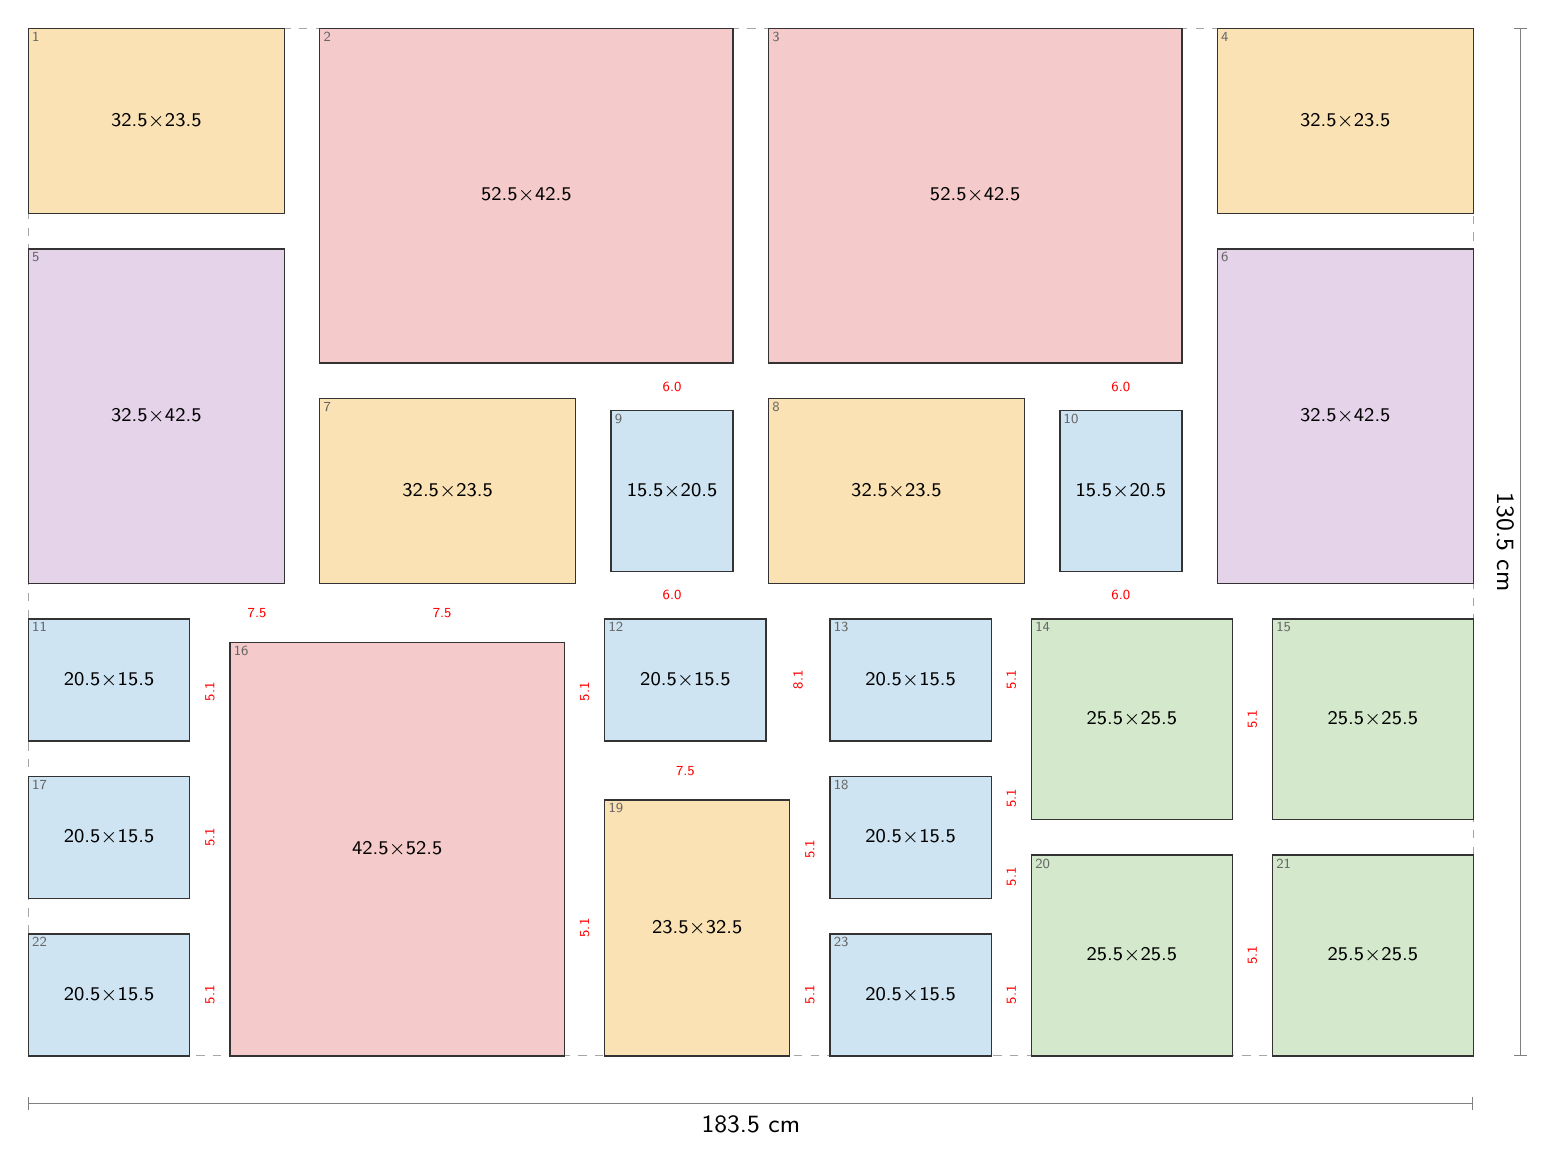
\begin{tikzpicture}[x=1mm, y=-1mm]
\draw[gray!70, dashed, line width=0.4pt] (0,0) rectangle (183.50,130.50);
\filldraw[fill=ft1, draw=black!80, line width=0.5pt] (0.00,0.00) rectangle (32.50,23.50);
\node[align=center, inner sep=0pt] at (16.25,11.75) {\scriptsize 32.5$\times$23.5};
\node[anchor=north west, inner sep=1.2pt, font=\tiny, text=black!60] at (0.00,0.00) {1};
\filldraw[fill=ft4, draw=black!80, line width=0.5pt] (37.00,0.00) rectangle (89.50,42.50);
\node[align=center, inner sep=0pt] at (63.25,21.25) {\scriptsize 52.5$\times$42.5};
\node[anchor=north west, inner sep=1.2pt, font=\tiny, text=black!60] at (37.00,0.00) {2};
\filldraw[fill=ft4, draw=black!80, line width=0.5pt] (94.00,0.00) rectangle (146.50,42.50);
\node[align=center, inner sep=0pt] at (120.25,21.25) {\scriptsize 52.5$\times$42.5};
\node[anchor=north west, inner sep=1.2pt, font=\tiny, text=black!60] at (94.00,0.00) {3};
\filldraw[fill=ft1, draw=black!80, line width=0.5pt] (151.00,0.00) rectangle (183.50,23.50);
\node[align=center, inner sep=0pt] at (167.25,11.75) {\scriptsize 32.5$\times$23.5};
\node[anchor=north west, inner sep=1.2pt, font=\tiny, text=black!60] at (151.00,0.00) {4};
\filldraw[fill=ft3, draw=black!80, line width=0.5pt] (0.00,28.00) rectangle (32.50,70.50);
\node[align=center, inner sep=0pt] at (16.25,49.25) {\scriptsize 32.5$\times$42.5};
\node[anchor=north west, inner sep=1.2pt, font=\tiny, text=black!60] at (0.00,28.00) {5};
\filldraw[fill=ft3, draw=black!80, line width=0.5pt] (151.00,28.00) rectangle (183.50,70.50);
\node[align=center, inner sep=0pt] at (167.25,49.25) {\scriptsize 32.5$\times$42.5};
\node[anchor=north west, inner sep=1.2pt, font=\tiny, text=black!60] at (151.00,28.00) {6};
\filldraw[fill=ft1, draw=black!80, line width=0.5pt] (37.00,47.00) rectangle (69.50,70.50);
\node[align=center, inner sep=0pt] at (53.25,58.75) {\scriptsize 32.5$\times$23.5};
\node[anchor=north west, inner sep=1.2pt, font=\tiny, text=black!60] at (37.00,47.00) {7};
\filldraw[fill=ft1, draw=black!80, line width=0.5pt] (94.00,47.00) rectangle (126.50,70.50);
\node[align=center, inner sep=0pt] at (110.25,58.75) {\scriptsize 32.5$\times$23.5};
\node[anchor=north west, inner sep=1.2pt, font=\tiny, text=black!60] at (94.00,47.00) {8};
\filldraw[fill=ft0, draw=black!80, line width=0.5pt] (74.00,48.50) rectangle (89.50,69.00);
\node[align=center, inner sep=0pt] at (81.75,58.75) {\scriptsize 15.5$\times$20.5};
\node[anchor=north west, inner sep=1.2pt, font=\tiny, text=black!60] at (74.00,48.50) {9};
\filldraw[fill=ft0, draw=black!80, line width=0.5pt] (131.00,48.50) rectangle (146.50,69.00);
\node[align=center, inner sep=0pt] at (138.75,58.75) {\scriptsize 15.5$\times$20.5};
\node[anchor=north west, inner sep=1.2pt, font=\tiny, text=black!60] at (131.00,48.50) {10};
\filldraw[fill=ft0, draw=black!80, line width=0.5pt] (0.00,75.00) rectangle (20.50,90.50);
\node[align=center, inner sep=0pt] at (10.25,82.75) {\scriptsize 20.5$\times$15.5};
\node[anchor=north west, inner sep=1.2pt, font=\tiny, text=black!60] at (0.00,75.00) {11};
\filldraw[fill=ft0, draw=black!80, line width=0.5pt] (73.20,75.00) rectangle (93.70,90.50);
\node[align=center, inner sep=0pt] at (83.45,82.75) {\scriptsize 20.5$\times$15.5};
\node[anchor=north west, inner sep=1.2pt, font=\tiny, text=black!60] at (73.20,75.00) {12};
\filldraw[fill=ft0, draw=black!80, line width=0.5pt] (101.80,75.00) rectangle (122.30,90.50);
\node[align=center, inner sep=0pt] at (112.05,82.75) {\scriptsize 20.5$\times$15.5};
\node[anchor=north west, inner sep=1.2pt, font=\tiny, text=black!60] at (101.80,75.00) {13};
\filldraw[fill=ft2, draw=black!80, line width=0.5pt] (127.40,75.00) rectangle (152.90,100.50);
\node[align=center, inner sep=0pt] at (140.15,87.75) {\scriptsize 25.5$\times$25.5};
\node[anchor=north west, inner sep=1.2pt, font=\tiny, text=black!60] at (127.40,75.00) {14};
\filldraw[fill=ft2, draw=black!80, line width=0.5pt] (158.00,75.00) rectangle (183.50,100.50);
\node[align=center, inner sep=0pt] at (170.75,87.75) {\scriptsize 25.5$\times$25.5};
\node[anchor=north west, inner sep=1.2pt, font=\tiny, text=black!60] at (158.00,75.00) {15};
\filldraw[fill=ft4, draw=black!80, line width=0.5pt] (25.60,78.00) rectangle (68.10,130.50);
\node[align=center, inner sep=0pt] at (46.85,104.25) {\scriptsize 42.5$\times$52.5};
\node[anchor=north west, inner sep=1.2pt, font=\tiny, text=black!60] at (25.60,78.00) {16};
\filldraw[fill=ft0, draw=black!80, line width=0.5pt] (0.00,95.00) rectangle (20.50,110.50);
\node[align=center, inner sep=0pt] at (10.25,102.75) {\scriptsize 20.5$\times$15.5};
\node[anchor=north west, inner sep=1.2pt, font=\tiny, text=black!60] at (0.00,95.00) {17};
\filldraw[fill=ft0, draw=black!80, line width=0.5pt] (101.80,95.00) rectangle (122.30,110.50);
\node[align=center, inner sep=0pt] at (112.05,102.75) {\scriptsize 20.5$\times$15.5};
\node[anchor=north west, inner sep=1.2pt, font=\tiny, text=black!60] at (101.80,95.00) {18};
\filldraw[fill=ft1, draw=black!80, line width=0.5pt] (73.20,98.00) rectangle (96.70,130.50);
\node[align=center, inner sep=0pt] at (84.95,114.25) {\scriptsize 23.5$\times$32.5};
\node[anchor=north west, inner sep=1.2pt, font=\tiny, text=black!60] at (73.20,98.00) {19};
\filldraw[fill=ft2, draw=black!80, line width=0.5pt] (127.40,105.00) rectangle (152.90,130.50);
\node[align=center, inner sep=0pt] at (140.15,117.75) {\scriptsize 25.5$\times$25.5};
\node[anchor=north west, inner sep=1.2pt, font=\tiny, text=black!60] at (127.40,105.00) {20};
\filldraw[fill=ft2, draw=black!80, line width=0.5pt] (158.00,105.00) rectangle (183.50,130.50);
\node[align=center, inner sep=0pt] at (170.75,117.75) {\scriptsize 25.5$\times$25.5};
\node[anchor=north west, inner sep=1.2pt, font=\tiny, text=black!60] at (158.00,105.00) {21};
\filldraw[fill=ft0, draw=black!80, line width=0.5pt] (0.00,115.00) rectangle (20.50,130.50);
\node[align=center, inner sep=0pt] at (10.25,122.75) {\scriptsize 20.5$\times$15.5};
\node[anchor=north west, inner sep=1.2pt, font=\tiny, text=black!60] at (0.00,115.00) {22};
\filldraw[fill=ft0, draw=black!80, line width=0.5pt] (101.80,115.00) rectangle (122.30,130.50);
\node[align=center, inner sep=0pt] at (112.05,122.75) {\scriptsize 20.5$\times$15.5};
\node[anchor=north west, inner sep=1.2pt, font=\tiny, text=black!60] at (101.80,115.00) {23};
\node[font=\tiny, text=red, fill=white, inner sep=0.3pt] at (81.75,45.50) {6.0};
\node[font=\tiny, text=red, fill=white, inner sep=0.3pt] at (138.75,45.50) {6.0};
\node[font=\tiny, text=red, fill=white, inner sep=0.3pt] at (29.05,74.25) {7.5};
\node[font=\tiny, text=red, fill=white, inner sep=0.3pt] at (52.55,74.25) {7.5};
\node[font=\tiny, text=red, fill=white, inner sep=0.3pt] at (81.75,72.00) {6.0};
\node[font=\tiny, text=red, fill=white, inner sep=0.3pt] at (138.75,72.00) {6.0};
\node[font=\tiny, text=red, fill=white, inner sep=0.3pt, rotate=90] at (23.05,84.25) {5.1};
\node[font=\tiny, text=red, fill=white, inner sep=0.3pt, rotate=90] at (97.75,82.75) {8.1};
\node[font=\tiny, text=red, fill=white, inner sep=0.3pt] at (83.45,94.25) {7.5};
\node[font=\tiny, text=red, fill=white, inner sep=0.3pt, rotate=90] at (124.85,82.75) {5.1};
\node[font=\tiny, text=red, fill=white, inner sep=0.3pt, rotate=90] at (155.45,87.75) {5.1};
\node[font=\tiny, text=red, fill=white, inner sep=0.3pt, rotate=90] at (70.65,84.25) {5.1};
\node[font=\tiny, text=red, fill=white, inner sep=0.3pt, rotate=90] at (70.65,114.25) {5.1};
\node[font=\tiny, text=red, fill=white, inner sep=0.3pt, rotate=90] at (23.05,102.75) {5.1};
\node[font=\tiny, text=red, fill=white, inner sep=0.3pt, rotate=90] at (124.85,97.75) {5.1};
\node[font=\tiny, text=red, fill=white, inner sep=0.3pt, rotate=90] at (124.85,107.75) {5.1};
\node[font=\tiny, text=red, fill=white, inner sep=0.3pt, rotate=90] at (99.25,104.25) {5.1};
\node[font=\tiny, text=red, fill=white, inner sep=0.3pt, rotate=90] at (99.25,122.75) {5.1};
\node[font=\tiny, text=red, fill=white, inner sep=0.3pt, rotate=90] at (155.45,117.75) {5.1};
\node[font=\tiny, text=red, fill=white, inner sep=0.3pt, rotate=90] at (23.05,122.75) {5.1};
\node[font=\tiny, text=red, fill=white, inner sep=0.3pt, rotate=90] at (124.85,122.75) {5.1};
\draw[Bar-Bar, gray] (0,136.50) -- (183.50,136.50) node[midway, below=1pt, font=\small, text=black] {183.5 cm};
\draw[Bar-Bar, gray] (189.50,0) -- (189.50,130.50) node[midway, right=1pt, font=\small, text=black, rotate=-90, anchor=north] {130.5 cm};
\end{tikzpicture}\\[4pt]
{\scriptsize Scale 1:10 (1 mm = 1 cm). Red numbers mark gaps that deviate from the nominal gap by more than 0.25 cm. Small grey numbers index the coordinate table.}
\end{minipage}\hfill
\begin{minipage}[t]{0.25\textwidth}\vspace{0pt}
\small
\begin{tabular}{@{}l l@{}}
\toprule
Outer size & 183.5 $\times$ 130.5 cm \\
Nominal gap & 4.5 cm \\
Actual gaps & 4.5 -- 8.1 cm \\
Max.\ deviation & 3.6 cm \\
Mean deviation & 0.60 cm \\
Border notches & none \\
Corners filled & 4 / 4 \\
Frames used & 23 of 28 \\
\bottomrule
\end{tabular}

\vspace{8pt}
\scriptsize
\begin{tabular}{@{}c l l r r@{}}
\toprule
 & outer w $\times$ h (cm) & & used & have \\
\midrule
\tikz[baseline=-0.6ex]\fill[ft0,draw=black!60] (0,0) rectangle (1.2ex,1.2ex); & 20.5$\times$15.5 & L & 7 & 9 \\
\tikz[baseline=-0.6ex]\fill[ft0,draw=black!60] (0,0) rectangle (1.2ex,1.2ex); & 15.5$\times$20.5 & P & 2 & 2 \\
\tikz[baseline=-0.6ex]\fill[ft3,draw=black!60] (0,0) rectangle (1.2ex,1.2ex); & 32.5$\times$42.5 & P & 2 & 2 \\
\tikz[baseline=-0.6ex]\fill[ft3,draw=black!60] (0,0) rectangle (1.2ex,1.2ex); & 42.5$\times$32.5 & L & 0 & 1 \\
\tikz[baseline=-0.6ex]\fill[ft1,draw=black!60] (0,0) rectangle (1.2ex,1.2ex); & 32.5$\times$23.5 & L & 4 & 5 \\
\tikz[baseline=-0.6ex]\fill[ft1,draw=black!60] (0,0) rectangle (1.2ex,1.2ex); & 23.5$\times$32.5 & P & 1 & 1 \\
\tikz[baseline=-0.6ex]\fill[ft2,draw=black!60] (0,0) rectangle (1.2ex,1.2ex); & 25.5$\times$25.5 &  & 4 & 5 \\
\tikz[baseline=-0.6ex]\fill[ft4,draw=black!60] (0,0) rectangle (1.2ex,1.2ex); & 42.5$\times$52.5 & P & 1 & 1 \\
\tikz[baseline=-0.6ex]\fill[ft4,draw=black!60] (0,0) rectangle (1.2ex,1.2ex); & 52.5$\times$42.5 & L & 2 & 2 \\
\bottomrule
\end{tabular}

\vspace{8pt}
{\bfseries Positions} (top-left corner, cm)\\[2pt]
\tiny
\begin{tabular}{@{}r l r r@{}}
\toprule
\# & frame w $\times$ h & x & y \\
\midrule
1 & 32.5 $\times$ 23.5 & 0.0 & 0.0 \\
2 & 52.5 $\times$ 42.5 & 37.0 & 0.0 \\
3 & 52.5 $\times$ 42.5 & 94.0 & 0.0 \\
4 & 32.5 $\times$ 23.5 & 151.0 & 0.0 \\
5 & 32.5 $\times$ 42.5 & 0.0 & 28.0 \\
6 & 32.5 $\times$ 42.5 & 151.0 & 28.0 \\
7 & 32.5 $\times$ 23.5 & 37.0 & 47.0 \\
8 & 32.5 $\times$ 23.5 & 94.0 & 47.0 \\
9 & 15.5 $\times$ 20.5 & 74.0 & 48.5 \\
10 & 15.5 $\times$ 20.5 & 131.0 & 48.5 \\
11 & 20.5 $\times$ 15.5 & 0.0 & 75.0 \\
12 & 20.5 $\times$ 15.5 & 73.2 & 75.0 \\
13 & 20.5 $\times$ 15.5 & 101.8 & 75.0 \\
14 & 25.5 $\times$ 25.5 & 127.4 & 75.0 \\
15 & 25.5 $\times$ 25.5 & 158.0 & 75.0 \\
16 & 42.5 $\times$ 52.5 & 25.6 & 78.0 \\
17 & 20.5 $\times$ 15.5 & 0.0 & 95.0 \\
18 & 20.5 $\times$ 15.5 & 101.8 & 95.0 \\
19 & 23.5 $\times$ 32.5 & 73.2 & 98.0 \\
20 & 25.5 $\times$ 25.5 & 127.4 & 105.0 \\
21 & 25.5 $\times$ 25.5 & 158.0 & 105.0 \\
22 & 20.5 $\times$ 15.5 & 0.0 & 115.0 \\
23 & 20.5 $\times$ 15.5 & 101.8 & 115.0 \\
\bottomrule
\end{tabular}
\end{minipage}
\clearpage

\begin{minipage}[t]{0.74\textwidth}\vspace{0pt}
{\LARGE\bfseries Layout 10}\hspace{1.5em}{\large 189.0 $\times$ 119.0 cm \quad gap 5 cm \quad 22 frames}\\[8pt]
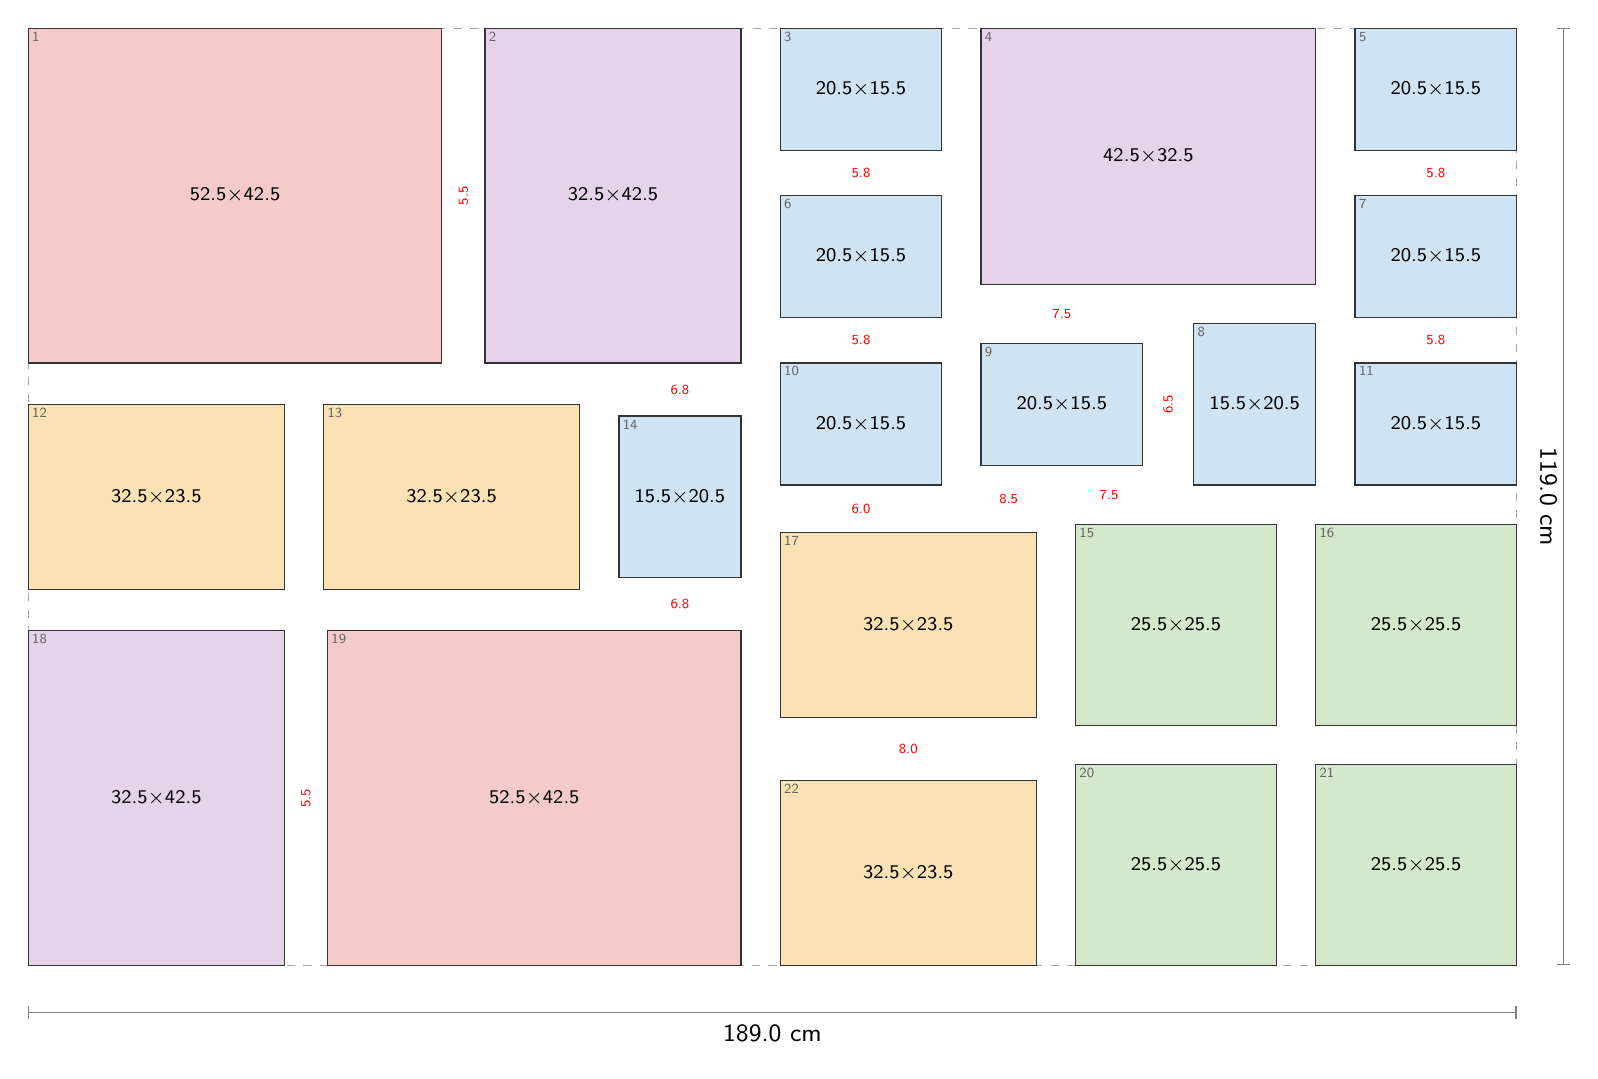
\begin{tikzpicture}[x=1mm, y=-1mm]
\draw[gray!70, dashed, line width=0.4pt] (0,0) rectangle (189.00,119.00);
\filldraw[fill=ft4, draw=black!80, line width=0.5pt] (0.00,0.00) rectangle (52.50,42.50);
\node[align=center, inner sep=0pt] at (26.25,21.25) {\scriptsize 52.5$\times$42.5};
\node[anchor=north west, inner sep=1.2pt, font=\tiny, text=black!60] at (0.00,0.00) {1};
\filldraw[fill=ft3, draw=black!80, line width=0.5pt] (58.00,0.00) rectangle (90.50,42.50);
\node[align=center, inner sep=0pt] at (74.25,21.25) {\scriptsize 32.5$\times$42.5};
\node[anchor=north west, inner sep=1.2pt, font=\tiny, text=black!60] at (58.00,0.00) {2};
\filldraw[fill=ft0, draw=black!80, line width=0.5pt] (95.50,0.00) rectangle (116.00,15.50);
\node[align=center, inner sep=0pt] at (105.75,7.75) {\scriptsize 20.5$\times$15.5};
\node[anchor=north west, inner sep=1.2pt, font=\tiny, text=black!60] at (95.50,0.00) {3};
\filldraw[fill=ft3, draw=black!80, line width=0.5pt] (121.00,0.00) rectangle (163.50,32.50);
\node[align=center, inner sep=0pt] at (142.25,16.25) {\scriptsize 42.5$\times$32.5};
\node[anchor=north west, inner sep=1.2pt, font=\tiny, text=black!60] at (121.00,0.00) {4};
\filldraw[fill=ft0, draw=black!80, line width=0.5pt] (168.50,0.00) rectangle (189.00,15.50);
\node[align=center, inner sep=0pt] at (178.75,7.75) {\scriptsize 20.5$\times$15.5};
\node[anchor=north west, inner sep=1.2pt, font=\tiny, text=black!60] at (168.50,0.00) {5};
\filldraw[fill=ft0, draw=black!80, line width=0.5pt] (95.50,21.25) rectangle (116.00,36.75);
\node[align=center, inner sep=0pt] at (105.75,29.00) {\scriptsize 20.5$\times$15.5};
\node[anchor=north west, inner sep=1.2pt, font=\tiny, text=black!60] at (95.50,21.25) {6};
\filldraw[fill=ft0, draw=black!80, line width=0.5pt] (168.50,21.25) rectangle (189.00,36.75);
\node[align=center, inner sep=0pt] at (178.75,29.00) {\scriptsize 20.5$\times$15.5};
\node[anchor=north west, inner sep=1.2pt, font=\tiny, text=black!60] at (168.50,21.25) {7};
\filldraw[fill=ft0, draw=black!80, line width=0.5pt] (148.00,37.50) rectangle (163.50,58.00);
\node[align=center, inner sep=0pt] at (155.75,47.75) {\scriptsize 15.5$\times$20.5};
\node[anchor=north west, inner sep=1.2pt, font=\tiny, text=black!60] at (148.00,37.50) {8};
\filldraw[fill=ft0, draw=black!80, line width=0.5pt] (121.00,40.00) rectangle (141.50,55.50);
\node[align=center, inner sep=0pt] at (131.25,47.75) {\scriptsize 20.5$\times$15.5};
\node[anchor=north west, inner sep=1.2pt, font=\tiny, text=black!60] at (121.00,40.00) {9};
\filldraw[fill=ft0, draw=black!80, line width=0.5pt] (95.50,42.50) rectangle (116.00,58.00);
\node[align=center, inner sep=0pt] at (105.75,50.25) {\scriptsize 20.5$\times$15.5};
\node[anchor=north west, inner sep=1.2pt, font=\tiny, text=black!60] at (95.50,42.50) {10};
\filldraw[fill=ft0, draw=black!80, line width=0.5pt] (168.50,42.50) rectangle (189.00,58.00);
\node[align=center, inner sep=0pt] at (178.75,50.25) {\scriptsize 20.5$\times$15.5};
\node[anchor=north west, inner sep=1.2pt, font=\tiny, text=black!60] at (168.50,42.50) {11};
\filldraw[fill=ft1, draw=black!80, line width=0.5pt] (0.00,47.75) rectangle (32.50,71.25);
\node[align=center, inner sep=0pt] at (16.25,59.50) {\scriptsize 32.5$\times$23.5};
\node[anchor=north west, inner sep=1.2pt, font=\tiny, text=black!60] at (0.00,47.75) {12};
\filldraw[fill=ft1, draw=black!80, line width=0.5pt] (37.50,47.75) rectangle (70.00,71.25);
\node[align=center, inner sep=0pt] at (53.75,59.50) {\scriptsize 32.5$\times$23.5};
\node[anchor=north west, inner sep=1.2pt, font=\tiny, text=black!60] at (37.50,47.75) {13};
\filldraw[fill=ft0, draw=black!80, line width=0.5pt] (75.00,49.25) rectangle (90.50,69.75);
\node[align=center, inner sep=0pt] at (82.75,59.50) {\scriptsize 15.5$\times$20.5};
\node[anchor=north west, inner sep=1.2pt, font=\tiny, text=black!60] at (75.00,49.25) {14};
\filldraw[fill=ft2, draw=black!80, line width=0.5pt] (133.00,63.00) rectangle (158.50,88.50);
\node[align=center, inner sep=0pt] at (145.75,75.75) {\scriptsize 25.5$\times$25.5};
\node[anchor=north west, inner sep=1.2pt, font=\tiny, text=black!60] at (133.00,63.00) {15};
\filldraw[fill=ft2, draw=black!80, line width=0.5pt] (163.50,63.00) rectangle (189.00,88.50);
\node[align=center, inner sep=0pt] at (176.25,75.75) {\scriptsize 25.5$\times$25.5};
\node[anchor=north west, inner sep=1.2pt, font=\tiny, text=black!60] at (163.50,63.00) {16};
\filldraw[fill=ft1, draw=black!80, line width=0.5pt] (95.50,64.00) rectangle (128.00,87.50);
\node[align=center, inner sep=0pt] at (111.75,75.75) {\scriptsize 32.5$\times$23.5};
\node[anchor=north west, inner sep=1.2pt, font=\tiny, text=black!60] at (95.50,64.00) {17};
\filldraw[fill=ft3, draw=black!80, line width=0.5pt] (0.00,76.50) rectangle (32.50,119.00);
\node[align=center, inner sep=0pt] at (16.25,97.75) {\scriptsize 32.5$\times$42.5};
\node[anchor=north west, inner sep=1.2pt, font=\tiny, text=black!60] at (0.00,76.50) {18};
\filldraw[fill=ft4, draw=black!80, line width=0.5pt] (38.00,76.50) rectangle (90.50,119.00);
\node[align=center, inner sep=0pt] at (64.25,97.75) {\scriptsize 52.5$\times$42.5};
\node[anchor=north west, inner sep=1.2pt, font=\tiny, text=black!60] at (38.00,76.50) {19};
\filldraw[fill=ft2, draw=black!80, line width=0.5pt] (133.00,93.50) rectangle (158.50,119.00);
\node[align=center, inner sep=0pt] at (145.75,106.25) {\scriptsize 25.5$\times$25.5};
\node[anchor=north west, inner sep=1.2pt, font=\tiny, text=black!60] at (133.00,93.50) {20};
\filldraw[fill=ft2, draw=black!80, line width=0.5pt] (163.50,93.50) rectangle (189.00,119.00);
\node[align=center, inner sep=0pt] at (176.25,106.25) {\scriptsize 25.5$\times$25.5};
\node[anchor=north west, inner sep=1.2pt, font=\tiny, text=black!60] at (163.50,93.50) {21};
\filldraw[fill=ft1, draw=black!80, line width=0.5pt] (95.50,95.50) rectangle (128.00,119.00);
\node[align=center, inner sep=0pt] at (111.75,107.25) {\scriptsize 32.5$\times$23.5};
\node[anchor=north west, inner sep=1.2pt, font=\tiny, text=black!60] at (95.50,95.50) {22};
\node[font=\tiny, text=red, fill=white, inner sep=0.3pt, rotate=90] at (55.25,21.25) {5.5};
\node[font=\tiny, text=red, fill=white, inner sep=0.3pt] at (82.75,45.88) {6.8};
\node[font=\tiny, text=red, fill=white, inner sep=0.3pt] at (105.75,18.38) {5.8};
\node[font=\tiny, text=red, fill=white, inner sep=0.3pt] at (131.25,36.25) {7.5};
\node[font=\tiny, text=red, fill=white, inner sep=0.3pt] at (178.75,18.38) {5.8};
\node[font=\tiny, text=red, fill=white, inner sep=0.3pt] at (105.75,39.62) {5.8};
\node[font=\tiny, text=red, fill=white, inner sep=0.3pt] at (178.75,39.62) {5.8};
\node[font=\tiny, text=red, fill=white, inner sep=0.3pt, rotate=90] at (144.75,47.75) {6.5};
\node[font=\tiny, text=red, fill=white, inner sep=0.3pt] at (137.25,59.25) {7.5};
\node[font=\tiny, text=red, fill=white, inner sep=0.3pt] at (124.50,59.75) {8.5};
\node[font=\tiny, text=red, fill=white, inner sep=0.3pt] at (105.75,61.00) {6.0};
\node[font=\tiny, text=red, fill=white, inner sep=0.3pt] at (82.75,73.12) {6.8};
\node[font=\tiny, text=red, fill=white, inner sep=0.3pt] at (111.75,91.50) {8.0};
\node[font=\tiny, text=red, fill=white, inner sep=0.3pt, rotate=90] at (35.25,97.75) {5.5};
\draw[Bar-Bar, gray] (0,125.00) -- (189.00,125.00) node[midway, below=1pt, font=\small, text=black] {189.0 cm};
\draw[Bar-Bar, gray] (195.00,0) -- (195.00,119.00) node[midway, right=1pt, font=\small, text=black, rotate=-90, anchor=north] {119.0 cm};
\end{tikzpicture}\\[4pt]
{\scriptsize Scale 1:10 (1 mm = 1 cm). Red numbers mark gaps that deviate from the nominal gap by more than 0.25 cm. Small grey numbers index the coordinate table.}
\end{minipage}\hfill
\begin{minipage}[t]{0.25\textwidth}\vspace{0pt}
\small
\begin{tabular}{@{}l l@{}}
\toprule
Outer size & 189.0 $\times$ 119.0 cm \\
Nominal gap & 5 cm \\
Actual gaps & 5.0 -- 8.5 cm \\
Max.\ deviation & 3.5 cm \\
Mean deviation & 0.54 cm \\
Border notches & none \\
Corners filled & 4 / 4 \\
Frames used & 22 of 28 \\
\bottomrule
\end{tabular}

\vspace{8pt}
\scriptsize
\begin{tabular}{@{}c l l r r@{}}
\toprule
 & outer w $\times$ h (cm) & & used & have \\
\midrule
\tikz[baseline=-0.6ex]\fill[ft0,draw=black!60] (0,0) rectangle (1.2ex,1.2ex); & 20.5$\times$15.5 & L & 7 & 9 \\
\tikz[baseline=-0.6ex]\fill[ft0,draw=black!60] (0,0) rectangle (1.2ex,1.2ex); & 15.5$\times$20.5 & P & 2 & 2 \\
\tikz[baseline=-0.6ex]\fill[ft3,draw=black!60] (0,0) rectangle (1.2ex,1.2ex); & 32.5$\times$42.5 & P & 2 & 2 \\
\tikz[baseline=-0.6ex]\fill[ft3,draw=black!60] (0,0) rectangle (1.2ex,1.2ex); & 42.5$\times$32.5 & L & 1 & 1 \\
\tikz[baseline=-0.6ex]\fill[ft1,draw=black!60] (0,0) rectangle (1.2ex,1.2ex); & 32.5$\times$23.5 & L & 4 & 5 \\
\tikz[baseline=-0.6ex]\fill[ft1,draw=black!60] (0,0) rectangle (1.2ex,1.2ex); & 23.5$\times$32.5 & P & 0 & 1 \\
\tikz[baseline=-0.6ex]\fill[ft2,draw=black!60] (0,0) rectangle (1.2ex,1.2ex); & 25.5$\times$25.5 &  & 4 & 5 \\
\tikz[baseline=-0.6ex]\fill[ft4,draw=black!60] (0,0) rectangle (1.2ex,1.2ex); & 42.5$\times$52.5 & P & 0 & 1 \\
\tikz[baseline=-0.6ex]\fill[ft4,draw=black!60] (0,0) rectangle (1.2ex,1.2ex); & 52.5$\times$42.5 & L & 2 & 2 \\
\bottomrule
\end{tabular}

\vspace{8pt}
{\bfseries Positions} (top-left corner, cm)\\[2pt]
\tiny
\begin{tabular}{@{}r l r r@{}}
\toprule
\# & frame w $\times$ h & x & y \\
\midrule
1 & 52.5 $\times$ 42.5 & 0.0 & 0.0 \\
2 & 32.5 $\times$ 42.5 & 58.0 & 0.0 \\
3 & 20.5 $\times$ 15.5 & 95.5 & 0.0 \\
4 & 42.5 $\times$ 32.5 & 121.0 & 0.0 \\
5 & 20.5 $\times$ 15.5 & 168.5 & 0.0 \\
6 & 20.5 $\times$ 15.5 & 95.5 & 21.2 \\
7 & 20.5 $\times$ 15.5 & 168.5 & 21.2 \\
8 & 15.5 $\times$ 20.5 & 148.0 & 37.5 \\
9 & 20.5 $\times$ 15.5 & 121.0 & 40.0 \\
10 & 20.5 $\times$ 15.5 & 95.5 & 42.5 \\
11 & 20.5 $\times$ 15.5 & 168.5 & 42.5 \\
12 & 32.5 $\times$ 23.5 & 0.0 & 47.8 \\
13 & 32.5 $\times$ 23.5 & 37.5 & 47.8 \\
14 & 15.5 $\times$ 20.5 & 75.0 & 49.2 \\
15 & 25.5 $\times$ 25.5 & 133.0 & 63.0 \\
16 & 25.5 $\times$ 25.5 & 163.5 & 63.0 \\
17 & 32.5 $\times$ 23.5 & 95.5 & 64.0 \\
18 & 32.5 $\times$ 42.5 & 0.0 & 76.5 \\
19 & 52.5 $\times$ 42.5 & 38.0 & 76.5 \\
20 & 25.5 $\times$ 25.5 & 133.0 & 93.5 \\
21 & 25.5 $\times$ 25.5 & 163.5 & 93.5 \\
22 & 32.5 $\times$ 23.5 & 95.5 & 95.5 \\
\bottomrule
\end{tabular}
\end{minipage}
\clearpage

\begin{minipage}[t]{0.74\textwidth}\vspace{0pt}
{\LARGE\bfseries Layout 11}\hspace{1.5em}{\large 189.5 $\times$ 116.5 cm \quad gap 2.5 cm \quad 21 frames}\\[8pt]
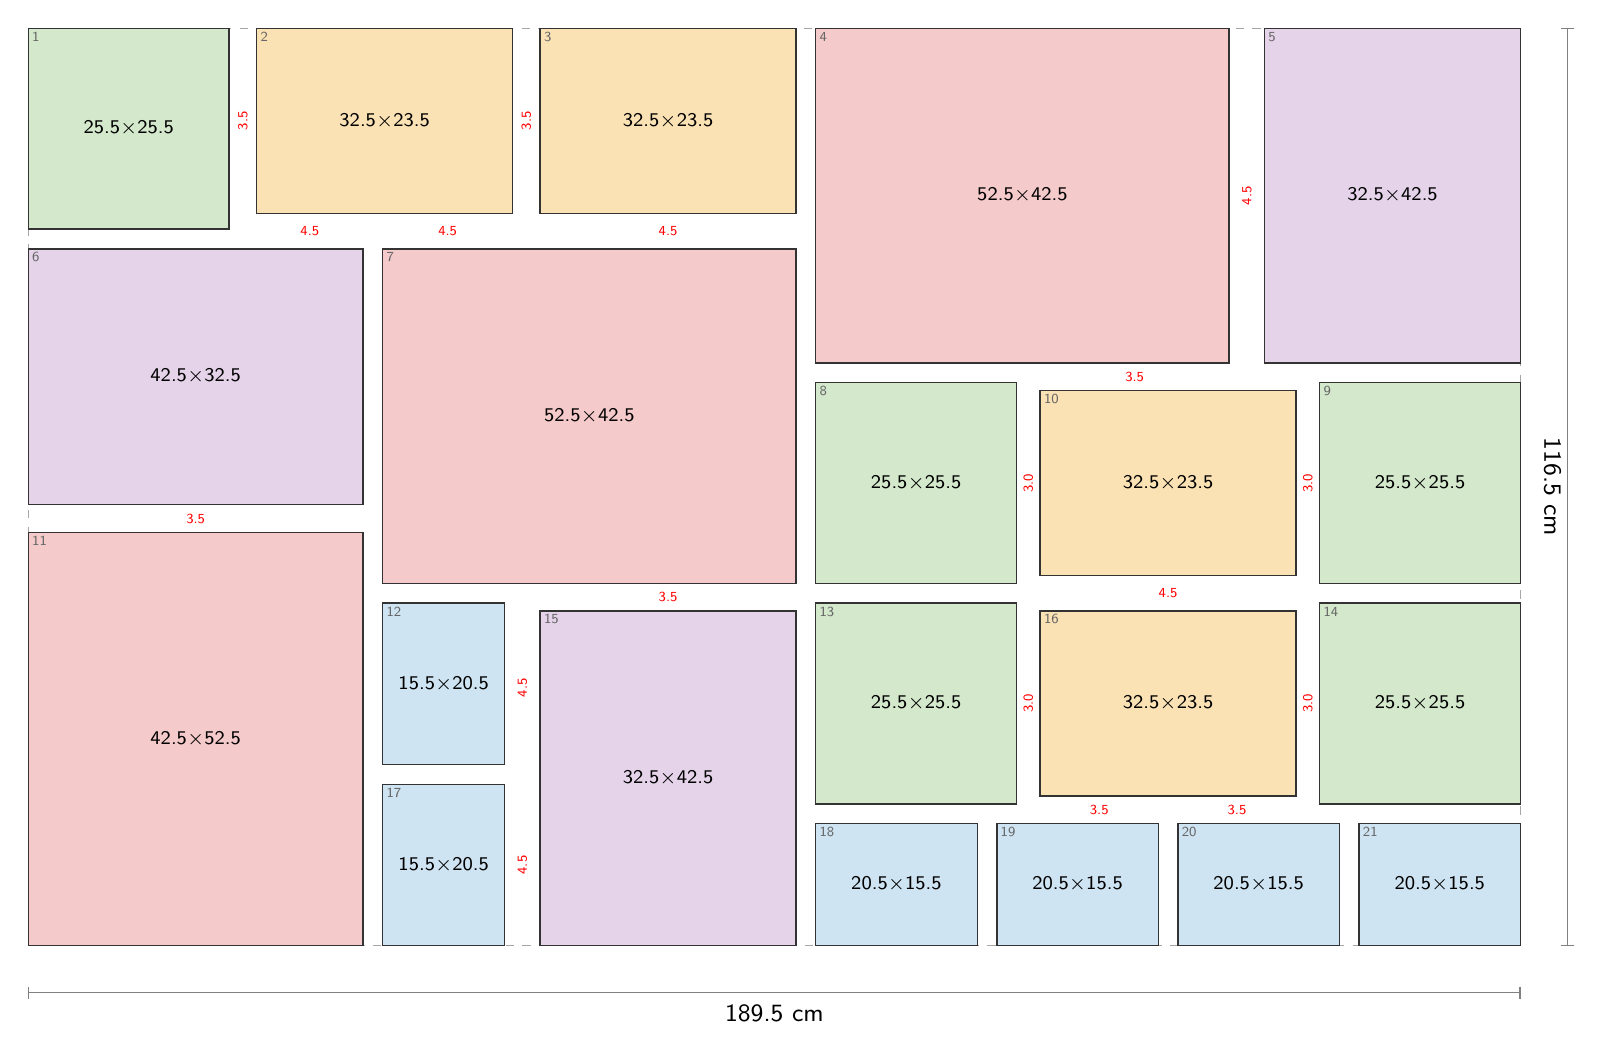
\begin{tikzpicture}[x=1mm, y=-1mm]
\draw[gray!70, dashed, line width=0.4pt] (0,0) rectangle (189.50,116.50);
\filldraw[fill=ft2, draw=black!80, line width=0.5pt] (0.00,0.00) rectangle (25.50,25.50);
\node[align=center, inner sep=0pt] at (12.75,12.75) {\scriptsize 25.5$\times$25.5};
\node[anchor=north west, inner sep=1.2pt, font=\tiny, text=black!60] at (0.00,0.00) {1};
\filldraw[fill=ft1, draw=black!80, line width=0.5pt] (29.00,0.00) rectangle (61.50,23.50);
\node[align=center, inner sep=0pt] at (45.25,11.75) {\scriptsize 32.5$\times$23.5};
\node[anchor=north west, inner sep=1.2pt, font=\tiny, text=black!60] at (29.00,0.00) {2};
\filldraw[fill=ft1, draw=black!80, line width=0.5pt] (65.00,0.00) rectangle (97.50,23.50);
\node[align=center, inner sep=0pt] at (81.25,11.75) {\scriptsize 32.5$\times$23.5};
\node[anchor=north west, inner sep=1.2pt, font=\tiny, text=black!60] at (65.00,0.00) {3};
\filldraw[fill=ft4, draw=black!80, line width=0.5pt] (100.00,0.00) rectangle (152.50,42.50);
\node[align=center, inner sep=0pt] at (126.25,21.25) {\scriptsize 52.5$\times$42.5};
\node[anchor=north west, inner sep=1.2pt, font=\tiny, text=black!60] at (100.00,0.00) {4};
\filldraw[fill=ft3, draw=black!80, line width=0.5pt] (157.00,0.00) rectangle (189.50,42.50);
\node[align=center, inner sep=0pt] at (173.25,21.25) {\scriptsize 32.5$\times$42.5};
\node[anchor=north west, inner sep=1.2pt, font=\tiny, text=black!60] at (157.00,0.00) {5};
\filldraw[fill=ft3, draw=black!80, line width=0.5pt] (0.00,28.00) rectangle (42.50,60.50);
\node[align=center, inner sep=0pt] at (21.25,44.25) {\scriptsize 42.5$\times$32.5};
\node[anchor=north west, inner sep=1.2pt, font=\tiny, text=black!60] at (0.00,28.00) {6};
\filldraw[fill=ft4, draw=black!80, line width=0.5pt] (45.00,28.00) rectangle (97.50,70.50);
\node[align=center, inner sep=0pt] at (71.25,49.25) {\scriptsize 52.5$\times$42.5};
\node[anchor=north west, inner sep=1.2pt, font=\tiny, text=black!60] at (45.00,28.00) {7};
\filldraw[fill=ft2, draw=black!80, line width=0.5pt] (100.00,45.00) rectangle (125.50,70.50);
\node[align=center, inner sep=0pt] at (112.75,57.75) {\scriptsize 25.5$\times$25.5};
\node[anchor=north west, inner sep=1.2pt, font=\tiny, text=black!60] at (100.00,45.00) {8};
\filldraw[fill=ft2, draw=black!80, line width=0.5pt] (164.00,45.00) rectangle (189.50,70.50);
\node[align=center, inner sep=0pt] at (176.75,57.75) {\scriptsize 25.5$\times$25.5};
\node[anchor=north west, inner sep=1.2pt, font=\tiny, text=black!60] at (164.00,45.00) {9};
\filldraw[fill=ft1, draw=black!80, line width=0.5pt] (128.50,46.00) rectangle (161.00,69.50);
\node[align=center, inner sep=0pt] at (144.75,57.75) {\scriptsize 32.5$\times$23.5};
\node[anchor=north west, inner sep=1.2pt, font=\tiny, text=black!60] at (128.50,46.00) {10};
\filldraw[fill=ft4, draw=black!80, line width=0.5pt] (0.00,64.00) rectangle (42.50,116.50);
\node[align=center, inner sep=0pt] at (21.25,90.25) {\scriptsize 42.5$\times$52.5};
\node[anchor=north west, inner sep=1.2pt, font=\tiny, text=black!60] at (0.00,64.00) {11};
\filldraw[fill=ft0, draw=black!80, line width=0.5pt] (45.00,73.00) rectangle (60.50,93.50);
\node[align=center, inner sep=0pt] at (52.75,83.25) {\scriptsize 15.5$\times$20.5};
\node[anchor=north west, inner sep=1.2pt, font=\tiny, text=black!60] at (45.00,73.00) {12};
\filldraw[fill=ft2, draw=black!80, line width=0.5pt] (100.00,73.00) rectangle (125.50,98.50);
\node[align=center, inner sep=0pt] at (112.75,85.75) {\scriptsize 25.5$\times$25.5};
\node[anchor=north west, inner sep=1.2pt, font=\tiny, text=black!60] at (100.00,73.00) {13};
\filldraw[fill=ft2, draw=black!80, line width=0.5pt] (164.00,73.00) rectangle (189.50,98.50);
\node[align=center, inner sep=0pt] at (176.75,85.75) {\scriptsize 25.5$\times$25.5};
\node[anchor=north west, inner sep=1.2pt, font=\tiny, text=black!60] at (164.00,73.00) {14};
\filldraw[fill=ft3, draw=black!80, line width=0.5pt] (65.00,74.00) rectangle (97.50,116.50);
\node[align=center, inner sep=0pt] at (81.25,95.25) {\scriptsize 32.5$\times$42.5};
\node[anchor=north west, inner sep=1.2pt, font=\tiny, text=black!60] at (65.00,74.00) {15};
\filldraw[fill=ft1, draw=black!80, line width=0.5pt] (128.50,74.00) rectangle (161.00,97.50);
\node[align=center, inner sep=0pt] at (144.75,85.75) {\scriptsize 32.5$\times$23.5};
\node[anchor=north west, inner sep=1.2pt, font=\tiny, text=black!60] at (128.50,74.00) {16};
\filldraw[fill=ft0, draw=black!80, line width=0.5pt] (45.00,96.00) rectangle (60.50,116.50);
\node[align=center, inner sep=0pt] at (52.75,106.25) {\scriptsize 15.5$\times$20.5};
\node[anchor=north west, inner sep=1.2pt, font=\tiny, text=black!60] at (45.00,96.00) {17};
\filldraw[fill=ft0, draw=black!80, line width=0.5pt] (100.00,101.00) rectangle (120.50,116.50);
\node[align=center, inner sep=0pt] at (110.25,108.75) {\scriptsize 20.5$\times$15.5};
\node[anchor=north west, inner sep=1.2pt, font=\tiny, text=black!60] at (100.00,101.00) {18};
\filldraw[fill=ft0, draw=black!80, line width=0.5pt] (123.00,101.00) rectangle (143.50,116.50);
\node[align=center, inner sep=0pt] at (133.25,108.75) {\scriptsize 20.5$\times$15.5};
\node[anchor=north west, inner sep=1.2pt, font=\tiny, text=black!60] at (123.00,101.00) {19};
\filldraw[fill=ft0, draw=black!80, line width=0.5pt] (146.00,101.00) rectangle (166.50,116.50);
\node[align=center, inner sep=0pt] at (156.25,108.75) {\scriptsize 20.5$\times$15.5};
\node[anchor=north west, inner sep=1.2pt, font=\tiny, text=black!60] at (146.00,101.00) {20};
\filldraw[fill=ft0, draw=black!80, line width=0.5pt] (169.00,101.00) rectangle (189.50,116.50);
\node[align=center, inner sep=0pt] at (179.25,108.75) {\scriptsize 20.5$\times$15.5};
\node[anchor=north west, inner sep=1.2pt, font=\tiny, text=black!60] at (169.00,101.00) {21};
\node[font=\tiny, text=red, fill=white, inner sep=0.3pt, rotate=90] at (27.25,11.75) {3.5};
\node[font=\tiny, text=red, fill=white, inner sep=0.3pt, rotate=90] at (63.25,11.75) {3.5};
\node[font=\tiny, text=red, fill=white, inner sep=0.3pt] at (35.75,25.75) {4.5};
\node[font=\tiny, text=red, fill=white, inner sep=0.3pt] at (53.25,25.75) {4.5};
\node[font=\tiny, text=red, fill=white, inner sep=0.3pt] at (81.25,25.75) {4.5};
\node[font=\tiny, text=red, fill=white, inner sep=0.3pt, rotate=90] at (154.75,21.25) {4.5};
\node[font=\tiny, text=red, fill=white, inner sep=0.3pt] at (140.50,44.25) {3.5};
\node[font=\tiny, text=red, fill=white, inner sep=0.3pt] at (21.25,62.25) {3.5};
\node[font=\tiny, text=red, fill=white, inner sep=0.3pt] at (81.25,72.25) {3.5};
\node[font=\tiny, text=red, fill=white, inner sep=0.3pt, rotate=90] at (127.00,57.75) {3.0};
\node[font=\tiny, text=red, fill=white, inner sep=0.3pt, rotate=90] at (162.50,57.75) {3.0};
\node[font=\tiny, text=red, fill=white, inner sep=0.3pt] at (144.75,71.75) {4.5};
\node[font=\tiny, text=red, fill=white, inner sep=0.3pt, rotate=90] at (62.75,83.75) {4.5};
\node[font=\tiny, text=red, fill=white, inner sep=0.3pt, rotate=90] at (127.00,85.75) {3.0};
\node[font=\tiny, text=red, fill=white, inner sep=0.3pt, rotate=90] at (162.50,85.75) {3.0};
\node[font=\tiny, text=red, fill=white, inner sep=0.3pt] at (136.00,99.25) {3.5};
\node[font=\tiny, text=red, fill=white, inner sep=0.3pt] at (153.50,99.25) {3.5};
\node[font=\tiny, text=red, fill=white, inner sep=0.3pt, rotate=90] at (62.75,106.25) {4.5};
\draw[Bar-Bar, gray] (0,122.50) -- (189.50,122.50) node[midway, below=1pt, font=\small, text=black] {189.5 cm};
\draw[Bar-Bar, gray] (195.50,0) -- (195.50,116.50) node[midway, right=1pt, font=\small, text=black, rotate=-90, anchor=north] {116.5 cm};
\end{tikzpicture}\\[4pt]
{\scriptsize Scale 1:10 (1 mm = 1 cm). Red numbers mark gaps that deviate from the nominal gap by more than 0.25 cm. Small grey numbers index the coordinate table.}
\end{minipage}\hfill
\begin{minipage}[t]{0.25\textwidth}\vspace{0pt}
\small
\begin{tabular}{@{}l l@{}}
\toprule
Outer size & 189.5 $\times$ 116.5 cm \\
Nominal gap & 2.5 cm \\
Actual gaps & 2.5 -- 4.5 cm \\
Max.\ deviation & 2.0 cm \\
Mean deviation & 0.59 cm \\
Border notches & top 4 cm, bottom 4 cm \\
Corners filled & 4 / 4 \\
Frames used & 21 of 28 \\
\bottomrule
\end{tabular}

\vspace{8pt}
\scriptsize
\begin{tabular}{@{}c l l r r@{}}
\toprule
 & outer w $\times$ h (cm) & & used & have \\
\midrule
\tikz[baseline=-0.6ex]\fill[ft0,draw=black!60] (0,0) rectangle (1.2ex,1.2ex); & 20.5$\times$15.5 & L & 4 & 9 \\
\tikz[baseline=-0.6ex]\fill[ft0,draw=black!60] (0,0) rectangle (1.2ex,1.2ex); & 15.5$\times$20.5 & P & 2 & 2 \\
\tikz[baseline=-0.6ex]\fill[ft3,draw=black!60] (0,0) rectangle (1.2ex,1.2ex); & 32.5$\times$42.5 & P & 2 & 2 \\
\tikz[baseline=-0.6ex]\fill[ft3,draw=black!60] (0,0) rectangle (1.2ex,1.2ex); & 42.5$\times$32.5 & L & 1 & 1 \\
\tikz[baseline=-0.6ex]\fill[ft1,draw=black!60] (0,0) rectangle (1.2ex,1.2ex); & 32.5$\times$23.5 & L & 4 & 5 \\
\tikz[baseline=-0.6ex]\fill[ft1,draw=black!60] (0,0) rectangle (1.2ex,1.2ex); & 23.5$\times$32.5 & P & 0 & 1 \\
\tikz[baseline=-0.6ex]\fill[ft2,draw=black!60] (0,0) rectangle (1.2ex,1.2ex); & 25.5$\times$25.5 &  & 5 & 5 \\
\tikz[baseline=-0.6ex]\fill[ft4,draw=black!60] (0,0) rectangle (1.2ex,1.2ex); & 42.5$\times$52.5 & P & 1 & 1 \\
\tikz[baseline=-0.6ex]\fill[ft4,draw=black!60] (0,0) rectangle (1.2ex,1.2ex); & 52.5$\times$42.5 & L & 2 & 2 \\
\bottomrule
\end{tabular}

\vspace{8pt}
{\bfseries Positions} (top-left corner, cm)\\[2pt]
\tiny
\begin{tabular}{@{}r l r r@{}}
\toprule
\# & frame w $\times$ h & x & y \\
\midrule
1 & 25.5 $\times$ 25.5 & 0.0 & 0.0 \\
2 & 32.5 $\times$ 23.5 & 29.0 & 0.0 \\
3 & 32.5 $\times$ 23.5 & 65.0 & 0.0 \\
4 & 52.5 $\times$ 42.5 & 100.0 & 0.0 \\
5 & 32.5 $\times$ 42.5 & 157.0 & 0.0 \\
6 & 42.5 $\times$ 32.5 & 0.0 & 28.0 \\
7 & 52.5 $\times$ 42.5 & 45.0 & 28.0 \\
8 & 25.5 $\times$ 25.5 & 100.0 & 45.0 \\
9 & 25.5 $\times$ 25.5 & 164.0 & 45.0 \\
10 & 32.5 $\times$ 23.5 & 128.5 & 46.0 \\
11 & 42.5 $\times$ 52.5 & 0.0 & 64.0 \\
12 & 15.5 $\times$ 20.5 & 45.0 & 73.0 \\
13 & 25.5 $\times$ 25.5 & 100.0 & 73.0 \\
14 & 25.5 $\times$ 25.5 & 164.0 & 73.0 \\
15 & 32.5 $\times$ 42.5 & 65.0 & 74.0 \\
16 & 32.5 $\times$ 23.5 & 128.5 & 74.0 \\
17 & 15.5 $\times$ 20.5 & 45.0 & 96.0 \\
18 & 20.5 $\times$ 15.5 & 100.0 & 101.0 \\
19 & 20.5 $\times$ 15.5 & 123.0 & 101.0 \\
20 & 20.5 $\times$ 15.5 & 146.0 & 101.0 \\
21 & 20.5 $\times$ 15.5 & 169.0 & 101.0 \\
\bottomrule
\end{tabular}
\end{minipage}
\clearpage

\begin{minipage}[t]{0.74\textwidth}\vspace{0pt}
{\LARGE\bfseries Layout 12}\hspace{1.5em}{\large 177.5 $\times$ 113.5 cm \quad gap 1.5 cm \quad 21 frames}\\[8pt]
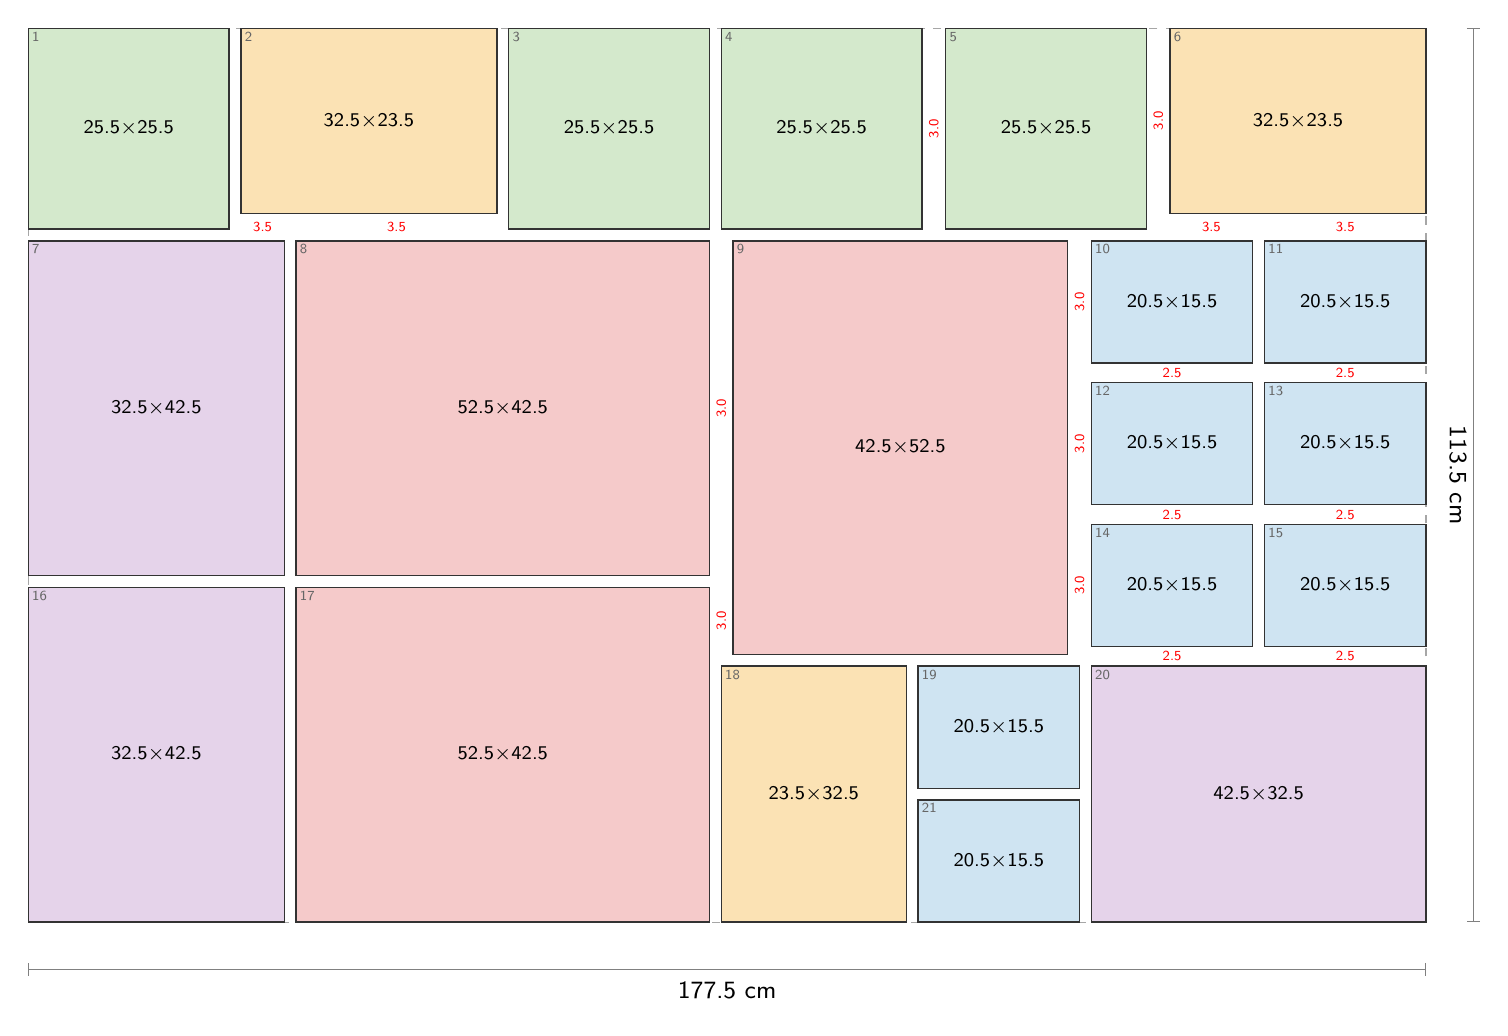
\begin{tikzpicture}[x=1mm, y=-1mm]
\draw[gray!70, dashed, line width=0.4pt] (0,0) rectangle (177.50,113.50);
\filldraw[fill=ft2, draw=black!80, line width=0.5pt] (0.00,0.00) rectangle (25.50,25.50);
\node[align=center, inner sep=0pt] at (12.75,12.75) {\scriptsize 25.5$\times$25.5};
\node[anchor=north west, inner sep=1.2pt, font=\tiny, text=black!60] at (0.00,0.00) {1};
\filldraw[fill=ft1, draw=black!80, line width=0.5pt] (27.00,0.00) rectangle (59.50,23.50);
\node[align=center, inner sep=0pt] at (43.25,11.75) {\scriptsize 32.5$\times$23.5};
\node[anchor=north west, inner sep=1.2pt, font=\tiny, text=black!60] at (27.00,0.00) {2};
\filldraw[fill=ft2, draw=black!80, line width=0.5pt] (61.00,0.00) rectangle (86.50,25.50);
\node[align=center, inner sep=0pt] at (73.75,12.75) {\scriptsize 25.5$\times$25.5};
\node[anchor=north west, inner sep=1.2pt, font=\tiny, text=black!60] at (61.00,0.00) {3};
\filldraw[fill=ft2, draw=black!80, line width=0.5pt] (88.00,0.00) rectangle (113.50,25.50);
\node[align=center, inner sep=0pt] at (100.75,12.75) {\scriptsize 25.5$\times$25.5};
\node[anchor=north west, inner sep=1.2pt, font=\tiny, text=black!60] at (88.00,0.00) {4};
\filldraw[fill=ft2, draw=black!80, line width=0.5pt] (116.50,0.00) rectangle (142.00,25.50);
\node[align=center, inner sep=0pt] at (129.25,12.75) {\scriptsize 25.5$\times$25.5};
\node[anchor=north west, inner sep=1.2pt, font=\tiny, text=black!60] at (116.50,0.00) {5};
\filldraw[fill=ft1, draw=black!80, line width=0.5pt] (145.00,0.00) rectangle (177.50,23.50);
\node[align=center, inner sep=0pt] at (161.25,11.75) {\scriptsize 32.5$\times$23.5};
\node[anchor=north west, inner sep=1.2pt, font=\tiny, text=black!60] at (145.00,0.00) {6};
\filldraw[fill=ft3, draw=black!80, line width=0.5pt] (0.00,27.00) rectangle (32.50,69.50);
\node[align=center, inner sep=0pt] at (16.25,48.25) {\scriptsize 32.5$\times$42.5};
\node[anchor=north west, inner sep=1.2pt, font=\tiny, text=black!60] at (0.00,27.00) {7};
\filldraw[fill=ft4, draw=black!80, line width=0.5pt] (34.00,27.00) rectangle (86.50,69.50);
\node[align=center, inner sep=0pt] at (60.25,48.25) {\scriptsize 52.5$\times$42.5};
\node[anchor=north west, inner sep=1.2pt, font=\tiny, text=black!60] at (34.00,27.00) {8};
\filldraw[fill=ft4, draw=black!80, line width=0.5pt] (89.50,27.00) rectangle (132.00,79.50);
\node[align=center, inner sep=0pt] at (110.75,53.25) {\scriptsize 42.5$\times$52.5};
\node[anchor=north west, inner sep=1.2pt, font=\tiny, text=black!60] at (89.50,27.00) {9};
\filldraw[fill=ft0, draw=black!80, line width=0.5pt] (135.00,27.00) rectangle (155.50,42.50);
\node[align=center, inner sep=0pt] at (145.25,34.75) {\scriptsize 20.5$\times$15.5};
\node[anchor=north west, inner sep=1.2pt, font=\tiny, text=black!60] at (135.00,27.00) {10};
\filldraw[fill=ft0, draw=black!80, line width=0.5pt] (157.00,27.00) rectangle (177.50,42.50);
\node[align=center, inner sep=0pt] at (167.25,34.75) {\scriptsize 20.5$\times$15.5};
\node[anchor=north west, inner sep=1.2pt, font=\tiny, text=black!60] at (157.00,27.00) {11};
\filldraw[fill=ft0, draw=black!80, line width=0.5pt] (135.00,45.00) rectangle (155.50,60.50);
\node[align=center, inner sep=0pt] at (145.25,52.75) {\scriptsize 20.5$\times$15.5};
\node[anchor=north west, inner sep=1.2pt, font=\tiny, text=black!60] at (135.00,45.00) {12};
\filldraw[fill=ft0, draw=black!80, line width=0.5pt] (157.00,45.00) rectangle (177.50,60.50);
\node[align=center, inner sep=0pt] at (167.25,52.75) {\scriptsize 20.5$\times$15.5};
\node[anchor=north west, inner sep=1.2pt, font=\tiny, text=black!60] at (157.00,45.00) {13};
\filldraw[fill=ft0, draw=black!80, line width=0.5pt] (135.00,63.00) rectangle (155.50,78.50);
\node[align=center, inner sep=0pt] at (145.25,70.75) {\scriptsize 20.5$\times$15.5};
\node[anchor=north west, inner sep=1.2pt, font=\tiny, text=black!60] at (135.00,63.00) {14};
\filldraw[fill=ft0, draw=black!80, line width=0.5pt] (157.00,63.00) rectangle (177.50,78.50);
\node[align=center, inner sep=0pt] at (167.25,70.75) {\scriptsize 20.5$\times$15.5};
\node[anchor=north west, inner sep=1.2pt, font=\tiny, text=black!60] at (157.00,63.00) {15};
\filldraw[fill=ft3, draw=black!80, line width=0.5pt] (0.00,71.00) rectangle (32.50,113.50);
\node[align=center, inner sep=0pt] at (16.25,92.25) {\scriptsize 32.5$\times$42.5};
\node[anchor=north west, inner sep=1.2pt, font=\tiny, text=black!60] at (0.00,71.00) {16};
\filldraw[fill=ft4, draw=black!80, line width=0.5pt] (34.00,71.00) rectangle (86.50,113.50);
\node[align=center, inner sep=0pt] at (60.25,92.25) {\scriptsize 52.5$\times$42.5};
\node[anchor=north west, inner sep=1.2pt, font=\tiny, text=black!60] at (34.00,71.00) {17};
\filldraw[fill=ft1, draw=black!80, line width=0.5pt] (88.00,81.00) rectangle (111.50,113.50);
\node[align=center, inner sep=0pt] at (99.75,97.25) {\scriptsize 23.5$\times$32.5};
\node[anchor=north west, inner sep=1.2pt, font=\tiny, text=black!60] at (88.00,81.00) {18};
\filldraw[fill=ft0, draw=black!80, line width=0.5pt] (113.00,81.00) rectangle (133.50,96.50);
\node[align=center, inner sep=0pt] at (123.25,88.75) {\scriptsize 20.5$\times$15.5};
\node[anchor=north west, inner sep=1.2pt, font=\tiny, text=black!60] at (113.00,81.00) {19};
\filldraw[fill=ft3, draw=black!80, line width=0.5pt] (135.00,81.00) rectangle (177.50,113.50);
\node[align=center, inner sep=0pt] at (156.25,97.25) {\scriptsize 42.5$\times$32.5};
\node[anchor=north west, inner sep=1.2pt, font=\tiny, text=black!60] at (135.00,81.00) {20};
\filldraw[fill=ft0, draw=black!80, line width=0.5pt] (113.00,98.00) rectangle (133.50,113.50);
\node[align=center, inner sep=0pt] at (123.25,105.75) {\scriptsize 20.5$\times$15.5};
\node[anchor=north west, inner sep=1.2pt, font=\tiny, text=black!60] at (113.00,98.00) {21};
\node[font=\tiny, text=red, fill=white, inner sep=0.3pt] at (29.75,25.25) {3.5};
\node[font=\tiny, text=red, fill=white, inner sep=0.3pt] at (46.75,25.25) {3.5};
\node[font=\tiny, text=red, fill=white, inner sep=0.3pt, rotate=90] at (115.00,12.75) {3.0};
\node[font=\tiny, text=red, fill=white, inner sep=0.3pt, rotate=90] at (143.50,11.75) {3.0};
\node[font=\tiny, text=red, fill=white, inner sep=0.3pt] at (150.25,25.25) {3.5};
\node[font=\tiny, text=red, fill=white, inner sep=0.3pt] at (167.25,25.25) {3.5};
\node[font=\tiny, text=red, fill=white, inner sep=0.3pt, rotate=90] at (88.00,48.25) {3.0};
\node[font=\tiny, text=red, fill=white, inner sep=0.3pt, rotate=90] at (133.50,34.75) {3.0};
\node[font=\tiny, text=red, fill=white, inner sep=0.3pt, rotate=90] at (133.50,52.75) {3.0};
\node[font=\tiny, text=red, fill=white, inner sep=0.3pt, rotate=90] at (133.50,70.75) {3.0};
\node[font=\tiny, text=red, fill=white, inner sep=0.3pt] at (145.25,43.75) {2.5};
\node[font=\tiny, text=red, fill=white, inner sep=0.3pt] at (167.25,43.75) {2.5};
\node[font=\tiny, text=red, fill=white, inner sep=0.3pt] at (145.25,61.75) {2.5};
\node[font=\tiny, text=red, fill=white, inner sep=0.3pt] at (167.25,61.75) {2.5};
\node[font=\tiny, text=red, fill=white, inner sep=0.3pt] at (145.25,79.75) {2.5};
\node[font=\tiny, text=red, fill=white, inner sep=0.3pt] at (167.25,79.75) {2.5};
\node[font=\tiny, text=red, fill=white, inner sep=0.3pt, rotate=90] at (88.00,75.25) {3.0};
\draw[Bar-Bar, gray] (0,119.50) -- (177.50,119.50) node[midway, below=1pt, font=\small, text=black] {177.5 cm};
\draw[Bar-Bar, gray] (183.50,0) -- (183.50,113.50) node[midway, right=1pt, font=\small, text=black, rotate=-90, anchor=north] {113.5 cm};
\end{tikzpicture}\\[4pt]
{\scriptsize Scale 1:10 (1 mm = 1 cm). Red numbers mark gaps that deviate from the nominal gap by more than 0.25 cm. Small grey numbers index the coordinate table.}
\end{minipage}\hfill
\begin{minipage}[t]{0.25\textwidth}\vspace{0pt}
\small
\begin{tabular}{@{}l l@{}}
\toprule
Outer size & 177.5 $\times$ 113.5 cm \\
Nominal gap & 1.5 cm \\
Actual gaps & 1.5 -- 3.5 cm \\
Max.\ deviation & 2.0 cm \\
Mean deviation & 0.61 cm \\
Border notches & top 6 cm, right 4 cm \\
Corners filled & 4 / 4 \\
Frames used & 21 of 28 \\
\bottomrule
\end{tabular}

\vspace{8pt}
\scriptsize
\begin{tabular}{@{}c l l r r@{}}
\toprule
 & outer w $\times$ h (cm) & & used & have \\
\midrule
\tikz[baseline=-0.6ex]\fill[ft0,draw=black!60] (0,0) rectangle (1.2ex,1.2ex); & 20.5$\times$15.5 & L & 8 & 9 \\
\tikz[baseline=-0.6ex]\fill[ft0,draw=black!60] (0,0) rectangle (1.2ex,1.2ex); & 15.5$\times$20.5 & P & 0 & 2 \\
\tikz[baseline=-0.6ex]\fill[ft3,draw=black!60] (0,0) rectangle (1.2ex,1.2ex); & 32.5$\times$42.5 & P & 2 & 2 \\
\tikz[baseline=-0.6ex]\fill[ft3,draw=black!60] (0,0) rectangle (1.2ex,1.2ex); & 42.5$\times$32.5 & L & 1 & 1 \\
\tikz[baseline=-0.6ex]\fill[ft1,draw=black!60] (0,0) rectangle (1.2ex,1.2ex); & 32.5$\times$23.5 & L & 2 & 5 \\
\tikz[baseline=-0.6ex]\fill[ft1,draw=black!60] (0,0) rectangle (1.2ex,1.2ex); & 23.5$\times$32.5 & P & 1 & 1 \\
\tikz[baseline=-0.6ex]\fill[ft2,draw=black!60] (0,0) rectangle (1.2ex,1.2ex); & 25.5$\times$25.5 &  & 4 & 5 \\
\tikz[baseline=-0.6ex]\fill[ft4,draw=black!60] (0,0) rectangle (1.2ex,1.2ex); & 42.5$\times$52.5 & P & 1 & 1 \\
\tikz[baseline=-0.6ex]\fill[ft4,draw=black!60] (0,0) rectangle (1.2ex,1.2ex); & 52.5$\times$42.5 & L & 2 & 2 \\
\bottomrule
\end{tabular}

\vspace{8pt}
{\bfseries Positions} (top-left corner, cm)\\[2pt]
\tiny
\begin{tabular}{@{}r l r r@{}}
\toprule
\# & frame w $\times$ h & x & y \\
\midrule
1 & 25.5 $\times$ 25.5 & 0.0 & 0.0 \\
2 & 32.5 $\times$ 23.5 & 27.0 & 0.0 \\
3 & 25.5 $\times$ 25.5 & 61.0 & 0.0 \\
4 & 25.5 $\times$ 25.5 & 88.0 & 0.0 \\
5 & 25.5 $\times$ 25.5 & 116.5 & 0.0 \\
6 & 32.5 $\times$ 23.5 & 145.0 & 0.0 \\
7 & 32.5 $\times$ 42.5 & 0.0 & 27.0 \\
8 & 52.5 $\times$ 42.5 & 34.0 & 27.0 \\
9 & 42.5 $\times$ 52.5 & 89.5 & 27.0 \\
10 & 20.5 $\times$ 15.5 & 135.0 & 27.0 \\
11 & 20.5 $\times$ 15.5 & 157.0 & 27.0 \\
12 & 20.5 $\times$ 15.5 & 135.0 & 45.0 \\
13 & 20.5 $\times$ 15.5 & 157.0 & 45.0 \\
14 & 20.5 $\times$ 15.5 & 135.0 & 63.0 \\
15 & 20.5 $\times$ 15.5 & 157.0 & 63.0 \\
16 & 32.5 $\times$ 42.5 & 0.0 & 71.0 \\
17 & 52.5 $\times$ 42.5 & 34.0 & 71.0 \\
18 & 23.5 $\times$ 32.5 & 88.0 & 81.0 \\
19 & 20.5 $\times$ 15.5 & 113.0 & 81.0 \\
20 & 42.5 $\times$ 32.5 & 135.0 & 81.0 \\
21 & 20.5 $\times$ 15.5 & 113.0 & 98.0 \\
\bottomrule
\end{tabular}
\end{minipage}
\clearpage

\begin{minipage}[t]{0.74\textwidth}\vspace{0pt}
{\LARGE\bfseries Layout 13}\hspace{1.5em}{\large 179.5 $\times$ 126.5 cm \quad gap 5.5 cm \quad 21 frames}\\[8pt]
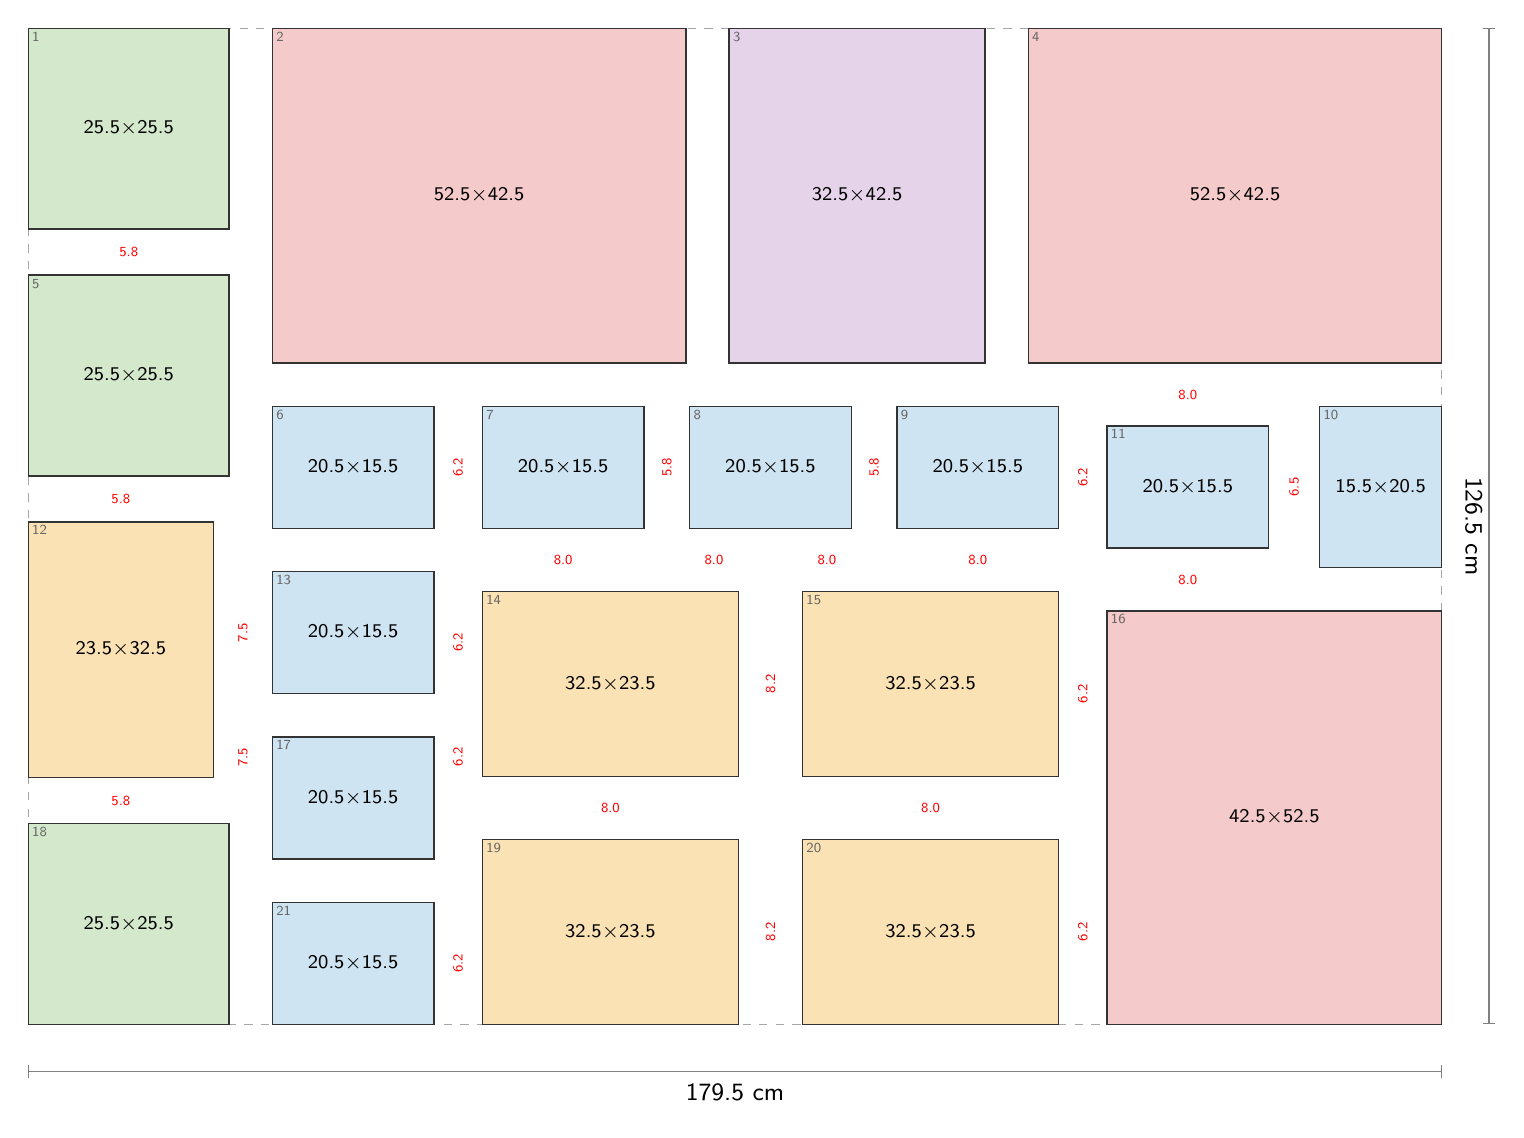
\begin{tikzpicture}[x=1mm, y=-1mm]
\draw[gray!70, dashed, line width=0.4pt] (0,0) rectangle (179.50,126.50);
\filldraw[fill=ft2, draw=black!80, line width=0.5pt] (0.00,0.00) rectangle (25.50,25.50);
\node[align=center, inner sep=0pt] at (12.75,12.75) {\scriptsize 25.5$\times$25.5};
\node[anchor=north west, inner sep=1.2pt, font=\tiny, text=black!60] at (0.00,0.00) {1};
\filldraw[fill=ft4, draw=black!80, line width=0.5pt] (31.00,0.00) rectangle (83.50,42.50);
\node[align=center, inner sep=0pt] at (57.25,21.25) {\scriptsize 52.5$\times$42.5};
\node[anchor=north west, inner sep=1.2pt, font=\tiny, text=black!60] at (31.00,0.00) {2};
\filldraw[fill=ft3, draw=black!80, line width=0.5pt] (89.00,0.00) rectangle (121.50,42.50);
\node[align=center, inner sep=0pt] at (105.25,21.25) {\scriptsize 32.5$\times$42.5};
\node[anchor=north west, inner sep=1.2pt, font=\tiny, text=black!60] at (89.00,0.00) {3};
\filldraw[fill=ft4, draw=black!80, line width=0.5pt] (127.00,0.00) rectangle (179.50,42.50);
\node[align=center, inner sep=0pt] at (153.25,21.25) {\scriptsize 52.5$\times$42.5};
\node[anchor=north west, inner sep=1.2pt, font=\tiny, text=black!60] at (127.00,0.00) {4};
\filldraw[fill=ft2, draw=black!80, line width=0.5pt] (0.00,31.33) rectangle (25.50,56.83);
\node[align=center, inner sep=0pt] at (12.75,44.08) {\scriptsize 25.5$\times$25.5};
\node[anchor=north west, inner sep=1.2pt, font=\tiny, text=black!60] at (0.00,31.33) {5};
\filldraw[fill=ft0, draw=black!80, line width=0.5pt] (31.00,48.00) rectangle (51.50,63.50);
\node[align=center, inner sep=0pt] at (41.25,55.75) {\scriptsize 20.5$\times$15.5};
\node[anchor=north west, inner sep=1.2pt, font=\tiny, text=black!60] at (31.00,48.00) {6};
\filldraw[fill=ft0, draw=black!80, line width=0.5pt] (57.67,48.00) rectangle (78.17,63.50);
\node[align=center, inner sep=0pt] at (67.92,55.75) {\scriptsize 20.5$\times$15.5};
\node[anchor=north west, inner sep=1.2pt, font=\tiny, text=black!60] at (57.67,48.00) {7};
\filldraw[fill=ft0, draw=black!80, line width=0.5pt] (84.00,48.00) rectangle (104.50,63.50);
\node[align=center, inner sep=0pt] at (94.25,55.75) {\scriptsize 20.5$\times$15.5};
\node[anchor=north west, inner sep=1.2pt, font=\tiny, text=black!60] at (84.00,48.00) {8};
\filldraw[fill=ft0, draw=black!80, line width=0.5pt] (110.33,48.00) rectangle (130.83,63.50);
\node[align=center, inner sep=0pt] at (120.58,55.75) {\scriptsize 20.5$\times$15.5};
\node[anchor=north west, inner sep=1.2pt, font=\tiny, text=black!60] at (110.33,48.00) {9};
\filldraw[fill=ft0, draw=black!80, line width=0.5pt] (164.00,48.00) rectangle (179.50,68.50);
\node[align=center, inner sep=0pt] at (171.75,58.25) {\scriptsize 15.5$\times$20.5};
\node[anchor=north west, inner sep=1.2pt, font=\tiny, text=black!60] at (164.00,48.00) {10};
\filldraw[fill=ft0, draw=black!80, line width=0.5pt] (137.00,50.50) rectangle (157.50,66.00);
\node[align=center, inner sep=0pt] at (147.25,58.25) {\scriptsize 20.5$\times$15.5};
\node[anchor=north west, inner sep=1.2pt, font=\tiny, text=black!60] at (137.00,50.50) {11};
\filldraw[fill=ft1, draw=black!80, line width=0.5pt] (0.00,62.67) rectangle (23.50,95.17);
\node[align=center, inner sep=0pt] at (11.75,78.92) {\scriptsize 23.5$\times$32.5};
\node[anchor=north west, inner sep=1.2pt, font=\tiny, text=black!60] at (0.00,62.67) {12};
\filldraw[fill=ft0, draw=black!80, line width=0.5pt] (31.00,69.00) rectangle (51.50,84.50);
\node[align=center, inner sep=0pt] at (41.25,76.75) {\scriptsize 20.5$\times$15.5};
\node[anchor=north west, inner sep=1.2pt, font=\tiny, text=black!60] at (31.00,69.00) {13};
\filldraw[fill=ft1, draw=black!80, line width=0.5pt] (57.67,71.50) rectangle (90.17,95.00);
\node[align=center, inner sep=0pt] at (73.92,83.25) {\scriptsize 32.5$\times$23.5};
\node[anchor=north west, inner sep=1.2pt, font=\tiny, text=black!60] at (57.67,71.50) {14};
\filldraw[fill=ft1, draw=black!80, line width=0.5pt] (98.33,71.50) rectangle (130.83,95.00);
\node[align=center, inner sep=0pt] at (114.58,83.25) {\scriptsize 32.5$\times$23.5};
\node[anchor=north west, inner sep=1.2pt, font=\tiny, text=black!60] at (98.33,71.50) {15};
\filldraw[fill=ft4, draw=black!80, line width=0.5pt] (137.00,74.00) rectangle (179.50,126.50);
\node[align=center, inner sep=0pt] at (158.25,100.25) {\scriptsize 42.5$\times$52.5};
\node[anchor=north west, inner sep=1.2pt, font=\tiny, text=black!60] at (137.00,74.00) {16};
\filldraw[fill=ft0, draw=black!80, line width=0.5pt] (31.00,90.00) rectangle (51.50,105.50);
\node[align=center, inner sep=0pt] at (41.25,97.75) {\scriptsize 20.5$\times$15.5};
\node[anchor=north west, inner sep=1.2pt, font=\tiny, text=black!60] at (31.00,90.00) {17};
\filldraw[fill=ft2, draw=black!80, line width=0.5pt] (0.00,101.00) rectangle (25.50,126.50);
\node[align=center, inner sep=0pt] at (12.75,113.75) {\scriptsize 25.5$\times$25.5};
\node[anchor=north west, inner sep=1.2pt, font=\tiny, text=black!60] at (0.00,101.00) {18};
\filldraw[fill=ft1, draw=black!80, line width=0.5pt] (57.67,103.00) rectangle (90.17,126.50);
\node[align=center, inner sep=0pt] at (73.92,114.75) {\scriptsize 32.5$\times$23.5};
\node[anchor=north west, inner sep=1.2pt, font=\tiny, text=black!60] at (57.67,103.00) {19};
\filldraw[fill=ft1, draw=black!80, line width=0.5pt] (98.33,103.00) rectangle (130.83,126.50);
\node[align=center, inner sep=0pt] at (114.58,114.75) {\scriptsize 32.5$\times$23.5};
\node[anchor=north west, inner sep=1.2pt, font=\tiny, text=black!60] at (98.33,103.00) {20};
\filldraw[fill=ft0, draw=black!80, line width=0.5pt] (31.00,111.00) rectangle (51.50,126.50);
\node[align=center, inner sep=0pt] at (41.25,118.75) {\scriptsize 20.5$\times$15.5};
\node[anchor=north west, inner sep=1.2pt, font=\tiny, text=black!60] at (31.00,111.00) {21};
\node[font=\tiny, text=red, fill=white, inner sep=0.3pt] at (12.75,28.42) {5.8};
\node[font=\tiny, text=red, fill=white, inner sep=0.3pt] at (147.25,46.50) {8.0};
\node[font=\tiny, text=red, fill=white, inner sep=0.3pt] at (11.75,59.75) {5.8};
\node[font=\tiny, text=red, fill=white, inner sep=0.3pt, rotate=90] at (54.58,55.75) {6.2};
\node[font=\tiny, text=red, fill=white, inner sep=0.3pt, rotate=90] at (81.08,55.75) {5.8};
\node[font=\tiny, text=red, fill=white, inner sep=0.3pt] at (67.92,67.50) {8.0};
\node[font=\tiny, text=red, fill=white, inner sep=0.3pt, rotate=90] at (107.42,55.75) {5.8};
\node[font=\tiny, text=red, fill=white, inner sep=0.3pt] at (87.08,67.50) {8.0};
\node[font=\tiny, text=red, fill=white, inner sep=0.3pt] at (101.42,67.50) {8.0};
\node[font=\tiny, text=red, fill=white, inner sep=0.3pt, rotate=90] at (133.92,57.00) {6.2};
\node[font=\tiny, text=red, fill=white, inner sep=0.3pt] at (120.58,67.50) {8.0};
\node[font=\tiny, text=red, fill=white, inner sep=0.3pt, rotate=90] at (160.75,58.25) {6.5};
\node[font=\tiny, text=red, fill=white, inner sep=0.3pt] at (147.25,70.00) {8.0};
\node[font=\tiny, text=red, fill=white, inner sep=0.3pt, rotate=90] at (27.25,76.75) {7.5};
\node[font=\tiny, text=red, fill=white, inner sep=0.3pt, rotate=90] at (27.25,92.58) {7.5};
\node[font=\tiny, text=red, fill=white, inner sep=0.3pt] at (11.75,98.08) {5.8};
\node[font=\tiny, text=red, fill=white, inner sep=0.3pt, rotate=90] at (54.58,78.00) {6.2};
\node[font=\tiny, text=red, fill=white, inner sep=0.3pt, rotate=90] at (94.25,83.25) {8.2};
\node[font=\tiny, text=red, fill=white, inner sep=0.3pt] at (73.92,99.00) {8.0};
\node[font=\tiny, text=red, fill=white, inner sep=0.3pt, rotate=90] at (133.92,84.50) {6.2};
\node[font=\tiny, text=red, fill=white, inner sep=0.3pt] at (114.58,99.00) {8.0};
\node[font=\tiny, text=red, fill=white, inner sep=0.3pt, rotate=90] at (54.58,92.50) {6.2};
\node[font=\tiny, text=red, fill=white, inner sep=0.3pt, rotate=90] at (94.25,114.75) {8.2};
\node[font=\tiny, text=red, fill=white, inner sep=0.3pt, rotate=90] at (133.92,114.75) {6.2};
\node[font=\tiny, text=red, fill=white, inner sep=0.3pt, rotate=90] at (54.58,118.75) {6.2};
\draw[Bar-Bar, gray] (0,132.50) -- (179.50,132.50) node[midway, below=1pt, font=\small, text=black] {179.5 cm};
\draw[Bar-Bar, gray] (185.50,0) -- (185.50,126.50) node[midway, right=1pt, font=\small, text=black, rotate=-90, anchor=north] {126.5 cm};
\end{tikzpicture}\\[4pt]
{\scriptsize Scale 1:10 (1 mm = 1 cm). Red numbers mark gaps that deviate from the nominal gap by more than 0.25 cm. Small grey numbers index the coordinate table.}
\end{minipage}\hfill
\begin{minipage}[t]{0.25\textwidth}\vspace{0pt}
\small
\begin{tabular}{@{}l l@{}}
\toprule
Outer size & 179.5 $\times$ 126.5 cm \\
Nominal gap & 5.5 cm \\
Actual gaps & 5.5 -- 8.2 cm \\
Max.\ deviation & 2.7 cm \\
Mean deviation & 0.92 cm \\
Border notches & bottom 8 cm \\
Corners filled & 4 / 4 \\
Frames used & 21 of 28 \\
\bottomrule
\end{tabular}

\vspace{8pt}
\scriptsize
\begin{tabular}{@{}c l l r r@{}}
\toprule
 & outer w $\times$ h (cm) & & used & have \\
\midrule
\tikz[baseline=-0.6ex]\fill[ft0,draw=black!60] (0,0) rectangle (1.2ex,1.2ex); & 20.5$\times$15.5 & L & 8 & 9 \\
\tikz[baseline=-0.6ex]\fill[ft0,draw=black!60] (0,0) rectangle (1.2ex,1.2ex); & 15.5$\times$20.5 & P & 1 & 2 \\
\tikz[baseline=-0.6ex]\fill[ft3,draw=black!60] (0,0) rectangle (1.2ex,1.2ex); & 32.5$\times$42.5 & P & 1 & 2 \\
\tikz[baseline=-0.6ex]\fill[ft3,draw=black!60] (0,0) rectangle (1.2ex,1.2ex); & 42.5$\times$32.5 & L & 0 & 1 \\
\tikz[baseline=-0.6ex]\fill[ft1,draw=black!60] (0,0) rectangle (1.2ex,1.2ex); & 32.5$\times$23.5 & L & 4 & 5 \\
\tikz[baseline=-0.6ex]\fill[ft1,draw=black!60] (0,0) rectangle (1.2ex,1.2ex); & 23.5$\times$32.5 & P & 1 & 1 \\
\tikz[baseline=-0.6ex]\fill[ft2,draw=black!60] (0,0) rectangle (1.2ex,1.2ex); & 25.5$\times$25.5 &  & 3 & 5 \\
\tikz[baseline=-0.6ex]\fill[ft4,draw=black!60] (0,0) rectangle (1.2ex,1.2ex); & 42.5$\times$52.5 & P & 1 & 1 \\
\tikz[baseline=-0.6ex]\fill[ft4,draw=black!60] (0,0) rectangle (1.2ex,1.2ex); & 52.5$\times$42.5 & L & 2 & 2 \\
\bottomrule
\end{tabular}

\vspace{8pt}
{\bfseries Positions} (top-left corner, cm)\\[2pt]
\tiny
\begin{tabular}{@{}r l r r@{}}
\toprule
\# & frame w $\times$ h & x & y \\
\midrule
1 & 25.5 $\times$ 25.5 & 0.0 & 0.0 \\
2 & 52.5 $\times$ 42.5 & 31.0 & 0.0 \\
3 & 32.5 $\times$ 42.5 & 89.0 & 0.0 \\
4 & 52.5 $\times$ 42.5 & 127.0 & 0.0 \\
5 & 25.5 $\times$ 25.5 & 0.0 & 31.3 \\
6 & 20.5 $\times$ 15.5 & 31.0 & 48.0 \\
7 & 20.5 $\times$ 15.5 & 57.7 & 48.0 \\
8 & 20.5 $\times$ 15.5 & 84.0 & 48.0 \\
9 & 20.5 $\times$ 15.5 & 110.3 & 48.0 \\
10 & 15.5 $\times$ 20.5 & 164.0 & 48.0 \\
11 & 20.5 $\times$ 15.5 & 137.0 & 50.5 \\
12 & 23.5 $\times$ 32.5 & 0.0 & 62.7 \\
13 & 20.5 $\times$ 15.5 & 31.0 & 69.0 \\
14 & 32.5 $\times$ 23.5 & 57.7 & 71.5 \\
15 & 32.5 $\times$ 23.5 & 98.3 & 71.5 \\
16 & 42.5 $\times$ 52.5 & 137.0 & 74.0 \\
17 & 20.5 $\times$ 15.5 & 31.0 & 90.0 \\
18 & 25.5 $\times$ 25.5 & 0.0 & 101.0 \\
19 & 32.5 $\times$ 23.5 & 57.7 & 103.0 \\
20 & 32.5 $\times$ 23.5 & 98.3 & 103.0 \\
21 & 20.5 $\times$ 15.5 & 31.0 & 111.0 \\
\bottomrule
\end{tabular}
\end{minipage}
\clearpage

\begin{minipage}[t]{0.74\textwidth}\vspace{0pt}
{\LARGE\bfseries Layout 14}\hspace{1.5em}{\large 181.5 $\times$ 113.5 cm \quad gap 1.5 cm \quad 20 frames}\\[8pt]
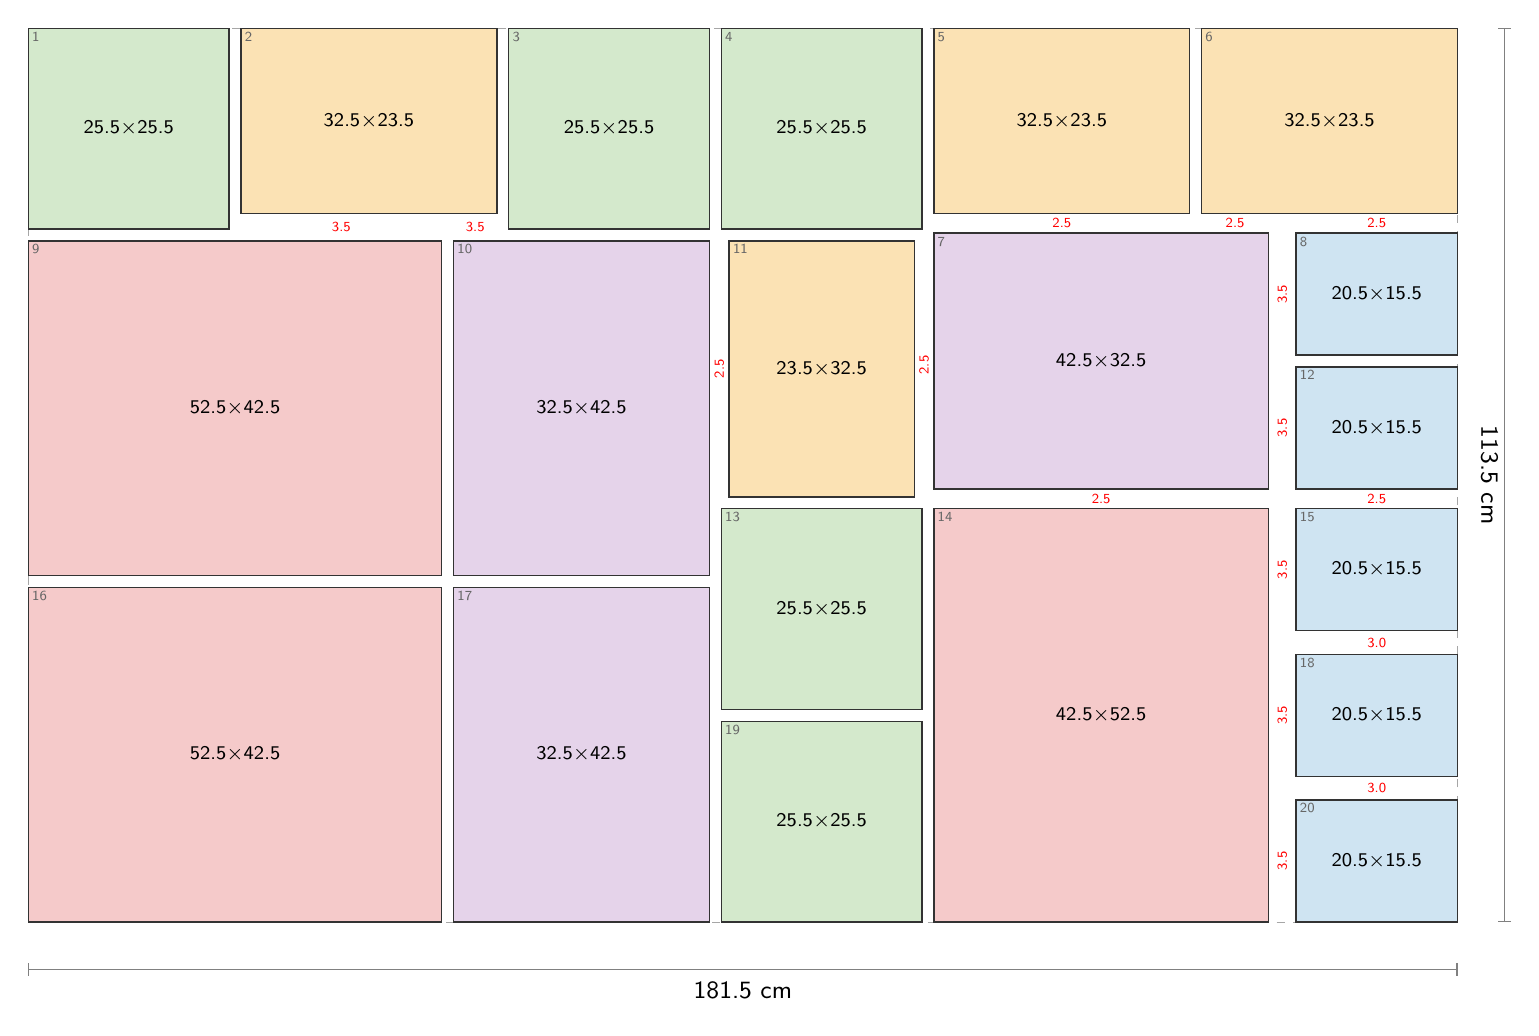
\begin{tikzpicture}[x=1mm, y=-1mm]
\draw[gray!70, dashed, line width=0.4pt] (0,0) rectangle (181.50,113.50);
\filldraw[fill=ft2, draw=black!80, line width=0.5pt] (0.00,0.00) rectangle (25.50,25.50);
\node[align=center, inner sep=0pt] at (12.75,12.75) {\scriptsize 25.5$\times$25.5};
\node[anchor=north west, inner sep=1.2pt, font=\tiny, text=black!60] at (0.00,0.00) {1};
\filldraw[fill=ft1, draw=black!80, line width=0.5pt] (27.00,0.00) rectangle (59.50,23.50);
\node[align=center, inner sep=0pt] at (43.25,11.75) {\scriptsize 32.5$\times$23.5};
\node[anchor=north west, inner sep=1.2pt, font=\tiny, text=black!60] at (27.00,0.00) {2};
\filldraw[fill=ft2, draw=black!80, line width=0.5pt] (61.00,0.00) rectangle (86.50,25.50);
\node[align=center, inner sep=0pt] at (73.75,12.75) {\scriptsize 25.5$\times$25.5};
\node[anchor=north west, inner sep=1.2pt, font=\tiny, text=black!60] at (61.00,0.00) {3};
\filldraw[fill=ft2, draw=black!80, line width=0.5pt] (88.00,0.00) rectangle (113.50,25.50);
\node[align=center, inner sep=0pt] at (100.75,12.75) {\scriptsize 25.5$\times$25.5};
\node[anchor=north west, inner sep=1.2pt, font=\tiny, text=black!60] at (88.00,0.00) {4};
\filldraw[fill=ft1, draw=black!80, line width=0.5pt] (115.00,0.00) rectangle (147.50,23.50);
\node[align=center, inner sep=0pt] at (131.25,11.75) {\scriptsize 32.5$\times$23.5};
\node[anchor=north west, inner sep=1.2pt, font=\tiny, text=black!60] at (115.00,0.00) {5};
\filldraw[fill=ft1, draw=black!80, line width=0.5pt] (149.00,0.00) rectangle (181.50,23.50);
\node[align=center, inner sep=0pt] at (165.25,11.75) {\scriptsize 32.5$\times$23.5};
\node[anchor=north west, inner sep=1.2pt, font=\tiny, text=black!60] at (149.00,0.00) {6};
\filldraw[fill=ft3, draw=black!80, line width=0.5pt] (115.00,26.00) rectangle (157.50,58.50);
\node[align=center, inner sep=0pt] at (136.25,42.25) {\scriptsize 42.5$\times$32.5};
\node[anchor=north west, inner sep=1.2pt, font=\tiny, text=black!60] at (115.00,26.00) {7};
\filldraw[fill=ft0, draw=black!80, line width=0.5pt] (161.00,26.00) rectangle (181.50,41.50);
\node[align=center, inner sep=0pt] at (171.25,33.75) {\scriptsize 20.5$\times$15.5};
\node[anchor=north west, inner sep=1.2pt, font=\tiny, text=black!60] at (161.00,26.00) {8};
\filldraw[fill=ft4, draw=black!80, line width=0.5pt] (0.00,27.00) rectangle (52.50,69.50);
\node[align=center, inner sep=0pt] at (26.25,48.25) {\scriptsize 52.5$\times$42.5};
\node[anchor=north west, inner sep=1.2pt, font=\tiny, text=black!60] at (0.00,27.00) {9};
\filldraw[fill=ft3, draw=black!80, line width=0.5pt] (54.00,27.00) rectangle (86.50,69.50);
\node[align=center, inner sep=0pt] at (70.25,48.25) {\scriptsize 32.5$\times$42.5};
\node[anchor=north west, inner sep=1.2pt, font=\tiny, text=black!60] at (54.00,27.00) {10};
\filldraw[fill=ft1, draw=black!80, line width=0.5pt] (89.00,27.00) rectangle (112.50,59.50);
\node[align=center, inner sep=0pt] at (100.75,43.25) {\scriptsize 23.5$\times$32.5};
\node[anchor=north west, inner sep=1.2pt, font=\tiny, text=black!60] at (89.00,27.00) {11};
\filldraw[fill=ft0, draw=black!80, line width=0.5pt] (161.00,43.00) rectangle (181.50,58.50);
\node[align=center, inner sep=0pt] at (171.25,50.75) {\scriptsize 20.5$\times$15.5};
\node[anchor=north west, inner sep=1.2pt, font=\tiny, text=black!60] at (161.00,43.00) {12};
\filldraw[fill=ft2, draw=black!80, line width=0.5pt] (88.00,61.00) rectangle (113.50,86.50);
\node[align=center, inner sep=0pt] at (100.75,73.75) {\scriptsize 25.5$\times$25.5};
\node[anchor=north west, inner sep=1.2pt, font=\tiny, text=black!60] at (88.00,61.00) {13};
\filldraw[fill=ft4, draw=black!80, line width=0.5pt] (115.00,61.00) rectangle (157.50,113.50);
\node[align=center, inner sep=0pt] at (136.25,87.25) {\scriptsize 42.5$\times$52.5};
\node[anchor=north west, inner sep=1.2pt, font=\tiny, text=black!60] at (115.00,61.00) {14};
\filldraw[fill=ft0, draw=black!80, line width=0.5pt] (161.00,61.00) rectangle (181.50,76.50);
\node[align=center, inner sep=0pt] at (171.25,68.75) {\scriptsize 20.5$\times$15.5};
\node[anchor=north west, inner sep=1.2pt, font=\tiny, text=black!60] at (161.00,61.00) {15};
\filldraw[fill=ft4, draw=black!80, line width=0.5pt] (0.00,71.00) rectangle (52.50,113.50);
\node[align=center, inner sep=0pt] at (26.25,92.25) {\scriptsize 52.5$\times$42.5};
\node[anchor=north west, inner sep=1.2pt, font=\tiny, text=black!60] at (0.00,71.00) {16};
\filldraw[fill=ft3, draw=black!80, line width=0.5pt] (54.00,71.00) rectangle (86.50,113.50);
\node[align=center, inner sep=0pt] at (70.25,92.25) {\scriptsize 32.5$\times$42.5};
\node[anchor=north west, inner sep=1.2pt, font=\tiny, text=black!60] at (54.00,71.00) {17};
\filldraw[fill=ft0, draw=black!80, line width=0.5pt] (161.00,79.50) rectangle (181.50,95.00);
\node[align=center, inner sep=0pt] at (171.25,87.25) {\scriptsize 20.5$\times$15.5};
\node[anchor=north west, inner sep=1.2pt, font=\tiny, text=black!60] at (161.00,79.50) {18};
\filldraw[fill=ft2, draw=black!80, line width=0.5pt] (88.00,88.00) rectangle (113.50,113.50);
\node[align=center, inner sep=0pt] at (100.75,100.75) {\scriptsize 25.5$\times$25.5};
\node[anchor=north west, inner sep=1.2pt, font=\tiny, text=black!60] at (88.00,88.00) {19};
\filldraw[fill=ft0, draw=black!80, line width=0.5pt] (161.00,98.00) rectangle (181.50,113.50);
\node[align=center, inner sep=0pt] at (171.25,105.75) {\scriptsize 20.5$\times$15.5};
\node[anchor=north west, inner sep=1.2pt, font=\tiny, text=black!60] at (161.00,98.00) {20};
\node[font=\tiny, text=red, fill=white, inner sep=0.3pt] at (39.75,25.25) {3.5};
\node[font=\tiny, text=red, fill=white, inner sep=0.3pt] at (56.75,25.25) {3.5};
\node[font=\tiny, text=red, fill=white, inner sep=0.3pt] at (131.25,24.75) {2.5};
\node[font=\tiny, text=red, fill=white, inner sep=0.3pt] at (153.25,24.75) {2.5};
\node[font=\tiny, text=red, fill=white, inner sep=0.3pt] at (171.25,24.75) {2.5};
\node[font=\tiny, text=red, fill=white, inner sep=0.3pt, rotate=90] at (159.25,33.75) {3.5};
\node[font=\tiny, text=red, fill=white, inner sep=0.3pt, rotate=90] at (159.25,50.75) {3.5};
\node[font=\tiny, text=red, fill=white, inner sep=0.3pt] at (136.25,59.75) {2.5};
\node[font=\tiny, text=red, fill=white, inner sep=0.3pt, rotate=90] at (87.75,43.25) {2.5};
\node[font=\tiny, text=red, fill=white, inner sep=0.3pt, rotate=90] at (113.75,42.75) {2.5};
\node[font=\tiny, text=red, fill=white, inner sep=0.3pt] at (171.25,59.75) {2.5};
\node[font=\tiny, text=red, fill=white, inner sep=0.3pt, rotate=90] at (159.25,68.75) {3.5};
\node[font=\tiny, text=red, fill=white, inner sep=0.3pt, rotate=90] at (159.25,87.25) {3.5};
\node[font=\tiny, text=red, fill=white, inner sep=0.3pt, rotate=90] at (159.25,105.75) {3.5};
\node[font=\tiny, text=red, fill=white, inner sep=0.3pt] at (171.25,78.00) {3.0};
\node[font=\tiny, text=red, fill=white, inner sep=0.3pt] at (171.25,96.50) {3.0};
\draw[Bar-Bar, gray] (0,119.50) -- (181.50,119.50) node[midway, below=1pt, font=\small, text=black] {181.5 cm};
\draw[Bar-Bar, gray] (187.50,0) -- (187.50,113.50) node[midway, right=1pt, font=\small, text=black, rotate=-90, anchor=north] {113.5 cm};
\end{tikzpicture}\\[4pt]
{\scriptsize Scale 1:10 (1 mm = 1 cm). Red numbers mark gaps that deviate from the nominal gap by more than 0.25 cm. Small grey numbers index the coordinate table.}
\end{minipage}\hfill
\begin{minipage}[t]{0.25\textwidth}\vspace{0pt}
\small
\begin{tabular}{@{}l l@{}}
\toprule
Outer size & 181.5 $\times$ 113.5 cm \\
Nominal gap & 1.5 cm \\
Actual gaps & 1.5 -- 3.5 cm \\
Max.\ deviation & 2.0 cm \\
Mean deviation & 0.67 cm \\
Border notches & bottom 4 cm, right 6 cm \\
Corners filled & 4 / 4 \\
Frames used & 20 of 28 \\
\bottomrule
\end{tabular}

\vspace{8pt}
\scriptsize
\begin{tabular}{@{}c l l r r@{}}
\toprule
 & outer w $\times$ h (cm) & & used & have \\
\midrule
\tikz[baseline=-0.6ex]\fill[ft0,draw=black!60] (0,0) rectangle (1.2ex,1.2ex); & 20.5$\times$15.5 & L & 5 & 9 \\
\tikz[baseline=-0.6ex]\fill[ft0,draw=black!60] (0,0) rectangle (1.2ex,1.2ex); & 15.5$\times$20.5 & P & 0 & 2 \\
\tikz[baseline=-0.6ex]\fill[ft3,draw=black!60] (0,0) rectangle (1.2ex,1.2ex); & 32.5$\times$42.5 & P & 2 & 2 \\
\tikz[baseline=-0.6ex]\fill[ft3,draw=black!60] (0,0) rectangle (1.2ex,1.2ex); & 42.5$\times$32.5 & L & 1 & 1 \\
\tikz[baseline=-0.6ex]\fill[ft1,draw=black!60] (0,0) rectangle (1.2ex,1.2ex); & 32.5$\times$23.5 & L & 3 & 5 \\
\tikz[baseline=-0.6ex]\fill[ft1,draw=black!60] (0,0) rectangle (1.2ex,1.2ex); & 23.5$\times$32.5 & P & 1 & 1 \\
\tikz[baseline=-0.6ex]\fill[ft2,draw=black!60] (0,0) rectangle (1.2ex,1.2ex); & 25.5$\times$25.5 &  & 5 & 5 \\
\tikz[baseline=-0.6ex]\fill[ft4,draw=black!60] (0,0) rectangle (1.2ex,1.2ex); & 42.5$\times$52.5 & P & 1 & 1 \\
\tikz[baseline=-0.6ex]\fill[ft4,draw=black!60] (0,0) rectangle (1.2ex,1.2ex); & 52.5$\times$42.5 & L & 2 & 2 \\
\bottomrule
\end{tabular}

\vspace{8pt}
{\bfseries Positions} (top-left corner, cm)\\[2pt]
\tiny
\begin{tabular}{@{}r l r r@{}}
\toprule
\# & frame w $\times$ h & x & y \\
\midrule
1 & 25.5 $\times$ 25.5 & 0.0 & 0.0 \\
2 & 32.5 $\times$ 23.5 & 27.0 & 0.0 \\
3 & 25.5 $\times$ 25.5 & 61.0 & 0.0 \\
4 & 25.5 $\times$ 25.5 & 88.0 & 0.0 \\
5 & 32.5 $\times$ 23.5 & 115.0 & 0.0 \\
6 & 32.5 $\times$ 23.5 & 149.0 & 0.0 \\
7 & 42.5 $\times$ 32.5 & 115.0 & 26.0 \\
8 & 20.5 $\times$ 15.5 & 161.0 & 26.0 \\
9 & 52.5 $\times$ 42.5 & 0.0 & 27.0 \\
10 & 32.5 $\times$ 42.5 & 54.0 & 27.0 \\
11 & 23.5 $\times$ 32.5 & 89.0 & 27.0 \\
12 & 20.5 $\times$ 15.5 & 161.0 & 43.0 \\
13 & 25.5 $\times$ 25.5 & 88.0 & 61.0 \\
14 & 42.5 $\times$ 52.5 & 115.0 & 61.0 \\
15 & 20.5 $\times$ 15.5 & 161.0 & 61.0 \\
16 & 52.5 $\times$ 42.5 & 0.0 & 71.0 \\
17 & 32.5 $\times$ 42.5 & 54.0 & 71.0 \\
18 & 20.5 $\times$ 15.5 & 161.0 & 79.5 \\
19 & 25.5 $\times$ 25.5 & 88.0 & 88.0 \\
20 & 20.5 $\times$ 15.5 & 161.0 & 98.0 \\
\bottomrule
\end{tabular}
\end{minipage}
\clearpage

\begin{minipage}[t]{0.74\textwidth}\vspace{0pt}
{\LARGE\bfseries Layout 15}\hspace{1.5em}{\large 191.0 $\times$ 103.5 cm \quad gap 6 cm \quad 16 frames}\\[8pt]
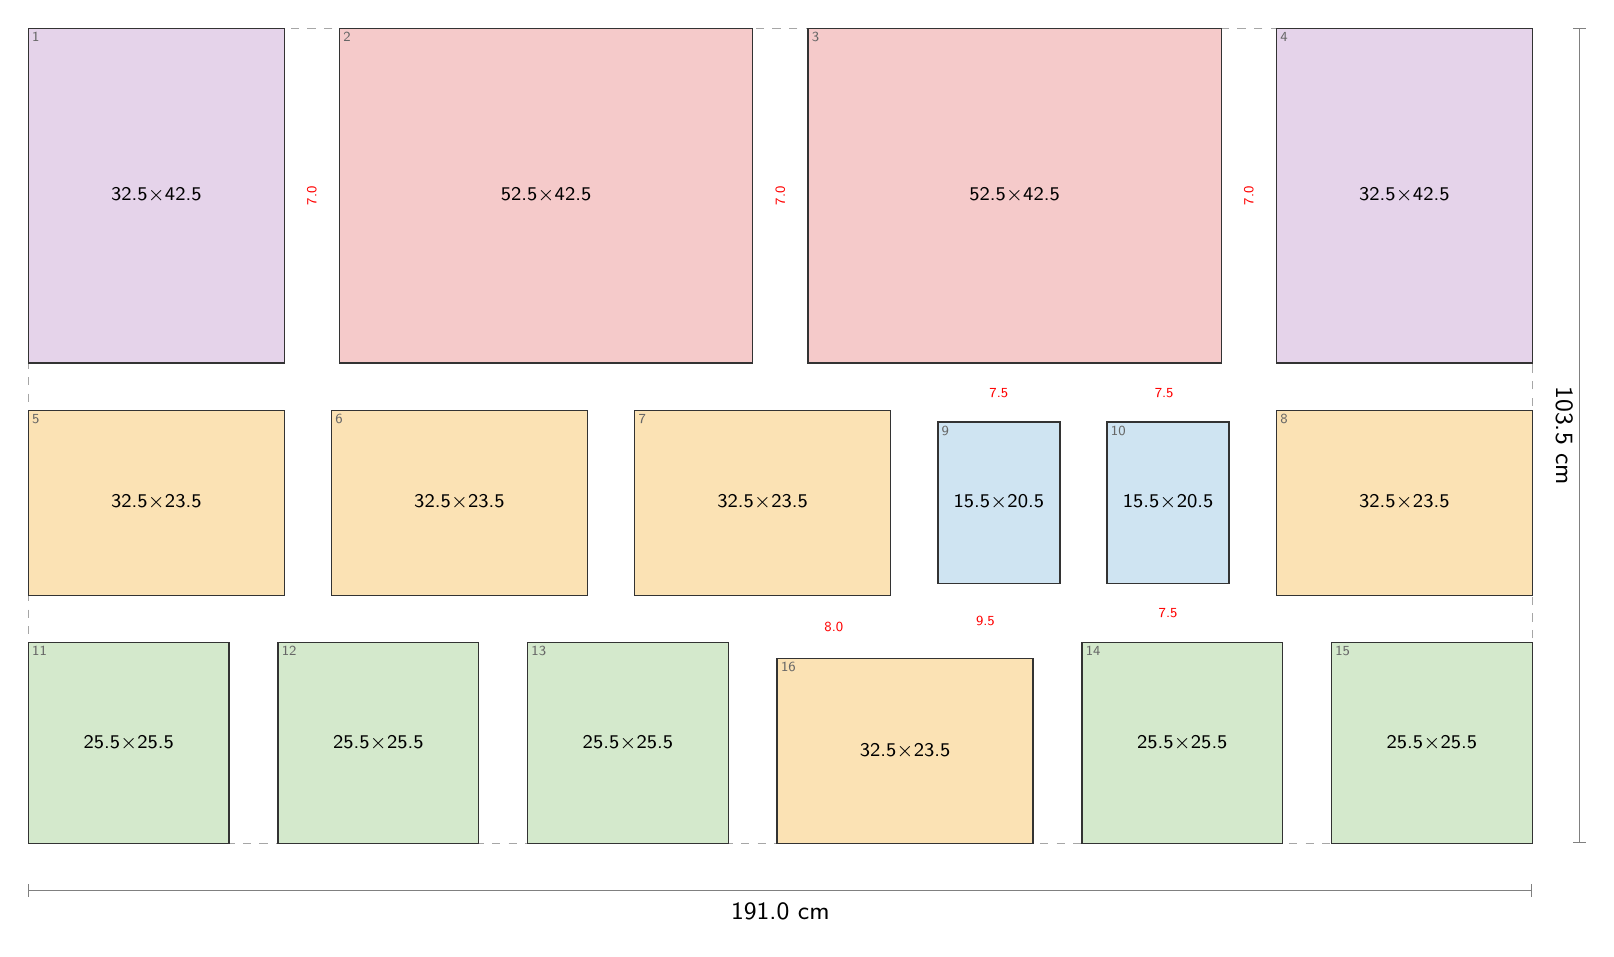
\begin{tikzpicture}[x=1mm, y=-1mm]
\draw[gray!70, dashed, line width=0.4pt] (0,0) rectangle (191.00,103.50);
\filldraw[fill=ft3, draw=black!80, line width=0.5pt] (0.00,0.00) rectangle (32.50,42.50);
\node[align=center, inner sep=0pt] at (16.25,21.25) {\scriptsize 32.5$\times$42.5};
\node[anchor=north west, inner sep=1.2pt, font=\tiny, text=black!60] at (0.00,0.00) {1};
\filldraw[fill=ft4, draw=black!80, line width=0.5pt] (39.50,0.00) rectangle (92.00,42.50);
\node[align=center, inner sep=0pt] at (65.75,21.25) {\scriptsize 52.5$\times$42.5};
\node[anchor=north west, inner sep=1.2pt, font=\tiny, text=black!60] at (39.50,0.00) {2};
\filldraw[fill=ft4, draw=black!80, line width=0.5pt] (99.00,0.00) rectangle (151.50,42.50);
\node[align=center, inner sep=0pt] at (125.25,21.25) {\scriptsize 52.5$\times$42.5};
\node[anchor=north west, inner sep=1.2pt, font=\tiny, text=black!60] at (99.00,0.00) {3};
\filldraw[fill=ft3, draw=black!80, line width=0.5pt] (158.50,0.00) rectangle (191.00,42.50);
\node[align=center, inner sep=0pt] at (174.75,21.25) {\scriptsize 32.5$\times$42.5};
\node[anchor=north west, inner sep=1.2pt, font=\tiny, text=black!60] at (158.50,0.00) {4};
\filldraw[fill=ft1, draw=black!80, line width=0.5pt] (0.00,48.50) rectangle (32.50,72.00);
\node[align=center, inner sep=0pt] at (16.25,60.25) {\scriptsize 32.5$\times$23.5};
\node[anchor=north west, inner sep=1.2pt, font=\tiny, text=black!60] at (0.00,48.50) {5};
\filldraw[fill=ft1, draw=black!80, line width=0.5pt] (38.50,48.50) rectangle (71.00,72.00);
\node[align=center, inner sep=0pt] at (54.75,60.25) {\scriptsize 32.5$\times$23.5};
\node[anchor=north west, inner sep=1.2pt, font=\tiny, text=black!60] at (38.50,48.50) {6};
\filldraw[fill=ft1, draw=black!80, line width=0.5pt] (77.00,48.50) rectangle (109.50,72.00);
\node[align=center, inner sep=0pt] at (93.25,60.25) {\scriptsize 32.5$\times$23.5};
\node[anchor=north west, inner sep=1.2pt, font=\tiny, text=black!60] at (77.00,48.50) {7};
\filldraw[fill=ft1, draw=black!80, line width=0.5pt] (158.50,48.50) rectangle (191.00,72.00);
\node[align=center, inner sep=0pt] at (174.75,60.25) {\scriptsize 32.5$\times$23.5};
\node[anchor=north west, inner sep=1.2pt, font=\tiny, text=black!60] at (158.50,48.50) {8};
\filldraw[fill=ft0, draw=black!80, line width=0.5pt] (115.50,50.00) rectangle (131.00,70.50);
\node[align=center, inner sep=0pt] at (123.25,60.25) {\scriptsize 15.5$\times$20.5};
\node[anchor=north west, inner sep=1.2pt, font=\tiny, text=black!60] at (115.50,50.00) {9};
\filldraw[fill=ft0, draw=black!80, line width=0.5pt] (137.00,50.00) rectangle (152.50,70.50);
\node[align=center, inner sep=0pt] at (144.75,60.25) {\scriptsize 15.5$\times$20.5};
\node[anchor=north west, inner sep=1.2pt, font=\tiny, text=black!60] at (137.00,50.00) {10};
\filldraw[fill=ft2, draw=black!80, line width=0.5pt] (0.00,78.00) rectangle (25.50,103.50);
\node[align=center, inner sep=0pt] at (12.75,90.75) {\scriptsize 25.5$\times$25.5};
\node[anchor=north west, inner sep=1.2pt, font=\tiny, text=black!60] at (0.00,78.00) {11};
\filldraw[fill=ft2, draw=black!80, line width=0.5pt] (31.70,78.00) rectangle (57.20,103.50);
\node[align=center, inner sep=0pt] at (44.45,90.75) {\scriptsize 25.5$\times$25.5};
\node[anchor=north west, inner sep=1.2pt, font=\tiny, text=black!60] at (31.70,78.00) {12};
\filldraw[fill=ft2, draw=black!80, line width=0.5pt] (63.40,78.00) rectangle (88.90,103.50);
\node[align=center, inner sep=0pt] at (76.15,90.75) {\scriptsize 25.5$\times$25.5};
\node[anchor=north west, inner sep=1.2pt, font=\tiny, text=black!60] at (63.40,78.00) {13};
\filldraw[fill=ft2, draw=black!80, line width=0.5pt] (133.80,78.00) rectangle (159.30,103.50);
\node[align=center, inner sep=0pt] at (146.55,90.75) {\scriptsize 25.5$\times$25.5};
\node[anchor=north west, inner sep=1.2pt, font=\tiny, text=black!60] at (133.80,78.00) {14};
\filldraw[fill=ft2, draw=black!80, line width=0.5pt] (165.50,78.00) rectangle (191.00,103.50);
\node[align=center, inner sep=0pt] at (178.25,90.75) {\scriptsize 25.5$\times$25.5};
\node[anchor=north west, inner sep=1.2pt, font=\tiny, text=black!60] at (165.50,78.00) {15};
\filldraw[fill=ft1, draw=black!80, line width=0.5pt] (95.10,80.00) rectangle (127.60,103.50);
\node[align=center, inner sep=0pt] at (111.35,91.75) {\scriptsize 32.5$\times$23.5};
\node[anchor=north west, inner sep=1.2pt, font=\tiny, text=black!60] at (95.10,80.00) {16};
\node[font=\tiny, text=red, fill=white, inner sep=0.3pt, rotate=90] at (36.00,21.25) {7.0};
\node[font=\tiny, text=red, fill=white, inner sep=0.3pt, rotate=90] at (95.50,21.25) {7.0};
\node[font=\tiny, text=red, fill=white, inner sep=0.3pt, rotate=90] at (155.00,21.25) {7.0};
\node[font=\tiny, text=red, fill=white, inner sep=0.3pt] at (123.25,46.25) {7.5};
\node[font=\tiny, text=red, fill=white, inner sep=0.3pt] at (144.25,46.25) {7.5};
\node[font=\tiny, text=red, fill=white, inner sep=0.3pt] at (102.30,76.00) {8.0};
\node[font=\tiny, text=red, fill=white, inner sep=0.3pt] at (121.55,75.25) {9.5};
\node[font=\tiny, text=red, fill=white, inner sep=0.3pt] at (144.75,74.25) {7.5};
\draw[Bar-Bar, gray] (0,109.50) -- (191.00,109.50) node[midway, below=1pt, font=\small, text=black] {191.0 cm};
\draw[Bar-Bar, gray] (197.00,0) -- (197.00,103.50) node[midway, right=1pt, font=\small, text=black, rotate=-90, anchor=north] {103.5 cm};
\end{tikzpicture}\\[4pt]
{\scriptsize Scale 1:10 (1 mm = 1 cm). Red numbers mark gaps that deviate from the nominal gap by more than 0.25 cm. Small grey numbers index the coordinate table.}
\end{minipage}\hfill
\begin{minipage}[t]{0.25\textwidth}\vspace{0pt}
\small
\begin{tabular}{@{}l l@{}}
\toprule
Outer size & 191.0 $\times$ 103.5 cm \\
Nominal gap & 6 cm \\
Actual gaps & 6.0 -- 9.5 cm \\
Max.\ deviation & 3.5 cm \\
Mean deviation & 0.50 cm \\
Border notches & none \\
Corners filled & 4 / 4 \\
Frames used & 16 of 28 \\
\bottomrule
\end{tabular}

\vspace{8pt}
\scriptsize
\begin{tabular}{@{}c l l r r@{}}
\toprule
 & outer w $\times$ h (cm) & & used & have \\
\midrule
\tikz[baseline=-0.6ex]\fill[ft0,draw=black!60] (0,0) rectangle (1.2ex,1.2ex); & 20.5$\times$15.5 & L & 0 & 9 \\
\tikz[baseline=-0.6ex]\fill[ft0,draw=black!60] (0,0) rectangle (1.2ex,1.2ex); & 15.5$\times$20.5 & P & 2 & 2 \\
\tikz[baseline=-0.6ex]\fill[ft3,draw=black!60] (0,0) rectangle (1.2ex,1.2ex); & 32.5$\times$42.5 & P & 2 & 2 \\
\tikz[baseline=-0.6ex]\fill[ft3,draw=black!60] (0,0) rectangle (1.2ex,1.2ex); & 42.5$\times$32.5 & L & 0 & 1 \\
\tikz[baseline=-0.6ex]\fill[ft1,draw=black!60] (0,0) rectangle (1.2ex,1.2ex); & 32.5$\times$23.5 & L & 5 & 5 \\
\tikz[baseline=-0.6ex]\fill[ft1,draw=black!60] (0,0) rectangle (1.2ex,1.2ex); & 23.5$\times$32.5 & P & 0 & 1 \\
\tikz[baseline=-0.6ex]\fill[ft2,draw=black!60] (0,0) rectangle (1.2ex,1.2ex); & 25.5$\times$25.5 &  & 5 & 5 \\
\tikz[baseline=-0.6ex]\fill[ft4,draw=black!60] (0,0) rectangle (1.2ex,1.2ex); & 42.5$\times$52.5 & P & 0 & 1 \\
\tikz[baseline=-0.6ex]\fill[ft4,draw=black!60] (0,0) rectangle (1.2ex,1.2ex); & 52.5$\times$42.5 & L & 2 & 2 \\
\bottomrule
\end{tabular}

\vspace{8pt}
{\bfseries Positions} (top-left corner, cm)\\[2pt]
\tiny
\begin{tabular}{@{}r l r r@{}}
\toprule
\# & frame w $\times$ h & x & y \\
\midrule
1 & 32.5 $\times$ 42.5 & 0.0 & 0.0 \\
2 & 52.5 $\times$ 42.5 & 39.5 & 0.0 \\
3 & 52.5 $\times$ 42.5 & 99.0 & 0.0 \\
4 & 32.5 $\times$ 42.5 & 158.5 & 0.0 \\
5 & 32.5 $\times$ 23.5 & 0.0 & 48.5 \\
6 & 32.5 $\times$ 23.5 & 38.5 & 48.5 \\
7 & 32.5 $\times$ 23.5 & 77.0 & 48.5 \\
8 & 32.5 $\times$ 23.5 & 158.5 & 48.5 \\
9 & 15.5 $\times$ 20.5 & 115.5 & 50.0 \\
10 & 15.5 $\times$ 20.5 & 137.0 & 50.0 \\
11 & 25.5 $\times$ 25.5 & 0.0 & 78.0 \\
12 & 25.5 $\times$ 25.5 & 31.7 & 78.0 \\
13 & 25.5 $\times$ 25.5 & 63.4 & 78.0 \\
14 & 25.5 $\times$ 25.5 & 133.8 & 78.0 \\
15 & 25.5 $\times$ 25.5 & 165.5 & 78.0 \\
16 & 32.5 $\times$ 23.5 & 95.1 & 80.0 \\
\bottomrule
\end{tabular}
\end{minipage}
\clearpage

\begin{minipage}[t]{0.74\textwidth}\vspace{0pt}
{\LARGE\bfseries Layout 16}\hspace{1.5em}{\large 182.5 $\times$ 123.5 cm \quad gap 1.5 cm \quad 26 frames}\\[8pt]
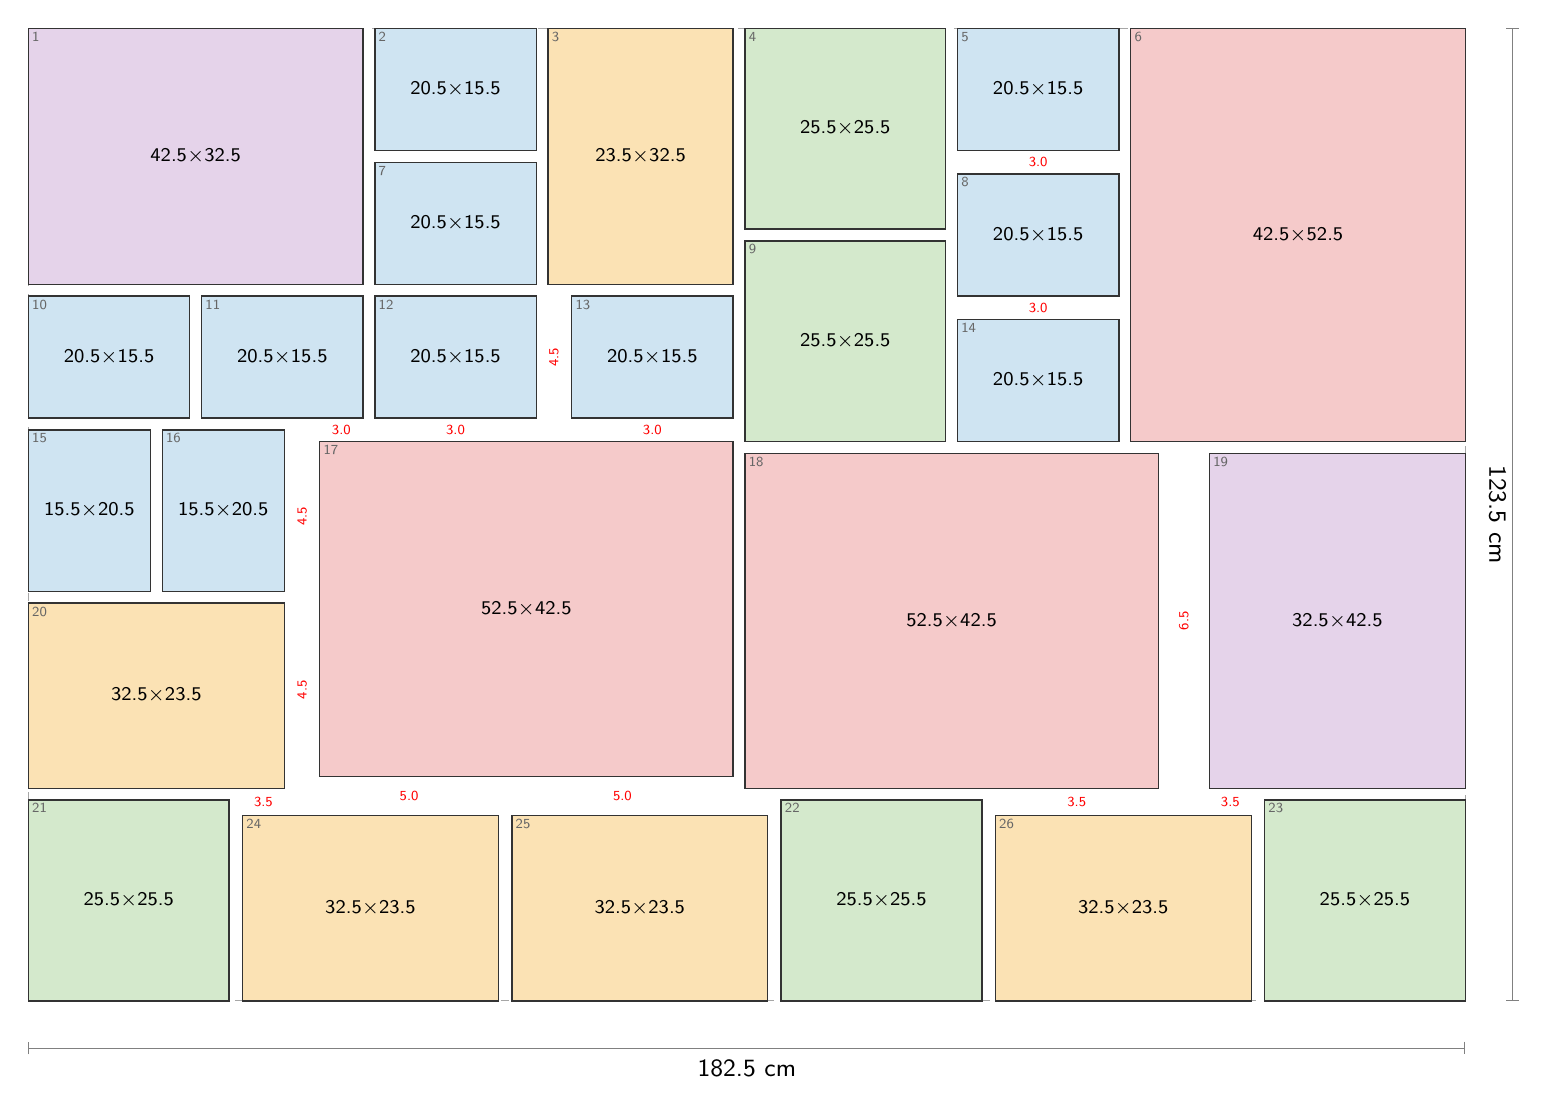
\begin{tikzpicture}[x=1mm, y=-1mm]
\draw[gray!70, dashed, line width=0.4pt] (0,0) rectangle (182.50,123.50);
\filldraw[fill=ft3, draw=black!80, line width=0.5pt] (0.00,0.00) rectangle (42.50,32.50);
\node[align=center, inner sep=0pt] at (21.25,16.25) {\scriptsize 42.5$\times$32.5};
\node[anchor=north west, inner sep=1.2pt, font=\tiny, text=black!60] at (0.00,0.00) {1};
\filldraw[fill=ft0, draw=black!80, line width=0.5pt] (44.00,0.00) rectangle (64.50,15.50);
\node[align=center, inner sep=0pt] at (54.25,7.75) {\scriptsize 20.5$\times$15.5};
\node[anchor=north west, inner sep=1.2pt, font=\tiny, text=black!60] at (44.00,0.00) {2};
\filldraw[fill=ft1, draw=black!80, line width=0.5pt] (66.00,0.00) rectangle (89.50,32.50);
\node[align=center, inner sep=0pt] at (77.75,16.25) {\scriptsize 23.5$\times$32.5};
\node[anchor=north west, inner sep=1.2pt, font=\tiny, text=black!60] at (66.00,0.00) {3};
\filldraw[fill=ft2, draw=black!80, line width=0.5pt] (91.00,0.00) rectangle (116.50,25.50);
\node[align=center, inner sep=0pt] at (103.75,12.75) {\scriptsize 25.5$\times$25.5};
\node[anchor=north west, inner sep=1.2pt, font=\tiny, text=black!60] at (91.00,0.00) {4};
\filldraw[fill=ft0, draw=black!80, line width=0.5pt] (118.00,0.00) rectangle (138.50,15.50);
\node[align=center, inner sep=0pt] at (128.25,7.75) {\scriptsize 20.5$\times$15.5};
\node[anchor=north west, inner sep=1.2pt, font=\tiny, text=black!60] at (118.00,0.00) {5};
\filldraw[fill=ft4, draw=black!80, line width=0.5pt] (140.00,0.00) rectangle (182.50,52.50);
\node[align=center, inner sep=0pt] at (161.25,26.25) {\scriptsize 42.5$\times$52.5};
\node[anchor=north west, inner sep=1.2pt, font=\tiny, text=black!60] at (140.00,0.00) {6};
\filldraw[fill=ft0, draw=black!80, line width=0.5pt] (44.00,17.00) rectangle (64.50,32.50);
\node[align=center, inner sep=0pt] at (54.25,24.75) {\scriptsize 20.5$\times$15.5};
\node[anchor=north west, inner sep=1.2pt, font=\tiny, text=black!60] at (44.00,17.00) {7};
\filldraw[fill=ft0, draw=black!80, line width=0.5pt] (118.00,18.50) rectangle (138.50,34.00);
\node[align=center, inner sep=0pt] at (128.25,26.25) {\scriptsize 20.5$\times$15.5};
\node[anchor=north west, inner sep=1.2pt, font=\tiny, text=black!60] at (118.00,18.50) {8};
\filldraw[fill=ft2, draw=black!80, line width=0.5pt] (91.00,27.00) rectangle (116.50,52.50);
\node[align=center, inner sep=0pt] at (103.75,39.75) {\scriptsize 25.5$\times$25.5};
\node[anchor=north west, inner sep=1.2pt, font=\tiny, text=black!60] at (91.00,27.00) {9};
\filldraw[fill=ft0, draw=black!80, line width=0.5pt] (0.00,34.00) rectangle (20.50,49.50);
\node[align=center, inner sep=0pt] at (10.25,41.75) {\scriptsize 20.5$\times$15.5};
\node[anchor=north west, inner sep=1.2pt, font=\tiny, text=black!60] at (0.00,34.00) {10};
\filldraw[fill=ft0, draw=black!80, line width=0.5pt] (22.00,34.00) rectangle (42.50,49.50);
\node[align=center, inner sep=0pt] at (32.25,41.75) {\scriptsize 20.5$\times$15.5};
\node[anchor=north west, inner sep=1.2pt, font=\tiny, text=black!60] at (22.00,34.00) {11};
\filldraw[fill=ft0, draw=black!80, line width=0.5pt] (44.00,34.00) rectangle (64.50,49.50);
\node[align=center, inner sep=0pt] at (54.25,41.75) {\scriptsize 20.5$\times$15.5};
\node[anchor=north west, inner sep=1.2pt, font=\tiny, text=black!60] at (44.00,34.00) {12};
\filldraw[fill=ft0, draw=black!80, line width=0.5pt] (69.00,34.00) rectangle (89.50,49.50);
\node[align=center, inner sep=0pt] at (79.25,41.75) {\scriptsize 20.5$\times$15.5};
\node[anchor=north west, inner sep=1.2pt, font=\tiny, text=black!60] at (69.00,34.00) {13};
\filldraw[fill=ft0, draw=black!80, line width=0.5pt] (118.00,37.00) rectangle (138.50,52.50);
\node[align=center, inner sep=0pt] at (128.25,44.75) {\scriptsize 20.5$\times$15.5};
\node[anchor=north west, inner sep=1.2pt, font=\tiny, text=black!60] at (118.00,37.00) {14};
\filldraw[fill=ft0, draw=black!80, line width=0.5pt] (0.00,51.00) rectangle (15.50,71.50);
\node[align=center, inner sep=0pt] at (7.75,61.25) {\scriptsize 15.5$\times$20.5};
\node[anchor=north west, inner sep=1.2pt, font=\tiny, text=black!60] at (0.00,51.00) {15};
\filldraw[fill=ft0, draw=black!80, line width=0.5pt] (17.00,51.00) rectangle (32.50,71.50);
\node[align=center, inner sep=0pt] at (24.75,61.25) {\scriptsize 15.5$\times$20.5};
\node[anchor=north west, inner sep=1.2pt, font=\tiny, text=black!60] at (17.00,51.00) {16};
\filldraw[fill=ft4, draw=black!80, line width=0.5pt] (37.00,52.50) rectangle (89.50,95.00);
\node[align=center, inner sep=0pt] at (63.25,73.75) {\scriptsize 52.5$\times$42.5};
\node[anchor=north west, inner sep=1.2pt, font=\tiny, text=black!60] at (37.00,52.50) {17};
\filldraw[fill=ft4, draw=black!80, line width=0.5pt] (91.00,54.00) rectangle (143.50,96.50);
\node[align=center, inner sep=0pt] at (117.25,75.25) {\scriptsize 52.5$\times$42.5};
\node[anchor=north west, inner sep=1.2pt, font=\tiny, text=black!60] at (91.00,54.00) {18};
\filldraw[fill=ft3, draw=black!80, line width=0.5pt] (150.00,54.00) rectangle (182.50,96.50);
\node[align=center, inner sep=0pt] at (166.25,75.25) {\scriptsize 32.5$\times$42.5};
\node[anchor=north west, inner sep=1.2pt, font=\tiny, text=black!60] at (150.00,54.00) {19};
\filldraw[fill=ft1, draw=black!80, line width=0.5pt] (0.00,73.00) rectangle (32.50,96.50);
\node[align=center, inner sep=0pt] at (16.25,84.75) {\scriptsize 32.5$\times$23.5};
\node[anchor=north west, inner sep=1.2pt, font=\tiny, text=black!60] at (0.00,73.00) {20};
\filldraw[fill=ft2, draw=black!80, line width=0.5pt] (0.00,98.00) rectangle (25.50,123.50);
\node[align=center, inner sep=0pt] at (12.75,110.75) {\scriptsize 25.5$\times$25.5};
\node[anchor=north west, inner sep=1.2pt, font=\tiny, text=black!60] at (0.00,98.00) {21};
\filldraw[fill=ft2, draw=black!80, line width=0.5pt] (95.60,98.00) rectangle (121.10,123.50);
\node[align=center, inner sep=0pt] at (108.35,110.75) {\scriptsize 25.5$\times$25.5};
\node[anchor=north west, inner sep=1.2pt, font=\tiny, text=black!60] at (95.60,98.00) {22};
\filldraw[fill=ft2, draw=black!80, line width=0.5pt] (157.00,98.00) rectangle (182.50,123.50);
\node[align=center, inner sep=0pt] at (169.75,110.75) {\scriptsize 25.5$\times$25.5};
\node[anchor=north west, inner sep=1.2pt, font=\tiny, text=black!60] at (157.00,98.00) {23};
\filldraw[fill=ft1, draw=black!80, line width=0.5pt] (27.20,100.00) rectangle (59.70,123.50);
\node[align=center, inner sep=0pt] at (43.45,111.75) {\scriptsize 32.5$\times$23.5};
\node[anchor=north west, inner sep=1.2pt, font=\tiny, text=black!60] at (27.20,100.00) {24};
\filldraw[fill=ft1, draw=black!80, line width=0.5pt] (61.40,100.00) rectangle (93.90,123.50);
\node[align=center, inner sep=0pt] at (77.65,111.75) {\scriptsize 32.5$\times$23.5};
\node[anchor=north west, inner sep=1.2pt, font=\tiny, text=black!60] at (61.40,100.00) {25};
\filldraw[fill=ft1, draw=black!80, line width=0.5pt] (122.80,100.00) rectangle (155.30,123.50);
\node[align=center, inner sep=0pt] at (139.05,111.75) {\scriptsize 32.5$\times$23.5};
\node[anchor=north west, inner sep=1.2pt, font=\tiny, text=black!60] at (122.80,100.00) {26};
\node[font=\tiny, text=red, fill=white, inner sep=0.3pt] at (128.25,17.00) {3.0};
\node[font=\tiny, text=red, fill=white, inner sep=0.3pt] at (128.25,35.50) {3.0};
\node[font=\tiny, text=red, fill=white, inner sep=0.3pt] at (39.75,51.00) {3.0};
\node[font=\tiny, text=red, fill=white, inner sep=0.3pt, rotate=90] at (66.75,41.75) {4.5};
\node[font=\tiny, text=red, fill=white, inner sep=0.3pt] at (54.25,51.00) {3.0};
\node[font=\tiny, text=red, fill=white, inner sep=0.3pt] at (79.25,51.00) {3.0};
\node[font=\tiny, text=red, fill=white, inner sep=0.3pt, rotate=90] at (34.75,62.00) {4.5};
\node[font=\tiny, text=red, fill=white, inner sep=0.3pt] at (48.35,97.50) {5.0};
\node[font=\tiny, text=red, fill=white, inner sep=0.3pt] at (75.45,97.50) {5.0};
\node[font=\tiny, text=red, fill=white, inner sep=0.3pt, rotate=90] at (146.75,75.25) {6.5};
\node[font=\tiny, text=red, fill=white, inner sep=0.3pt] at (133.15,98.25) {3.5};
\node[font=\tiny, text=red, fill=white, inner sep=0.3pt] at (152.65,98.25) {3.5};
\node[font=\tiny, text=red, fill=white, inner sep=0.3pt, rotate=90] at (34.75,84.00) {4.5};
\node[font=\tiny, text=red, fill=white, inner sep=0.3pt] at (29.85,98.25) {3.5};
\draw[Bar-Bar, gray] (0,129.50) -- (182.50,129.50) node[midway, below=1pt, font=\small, text=black] {182.5 cm};
\draw[Bar-Bar, gray] (188.50,0) -- (188.50,123.50) node[midway, right=1pt, font=\small, text=black, rotate=-90, anchor=north] {123.5 cm};
\end{tikzpicture}\\[4pt]
{\scriptsize Scale 1:10 (1 mm = 1 cm). Red numbers mark gaps that deviate from the nominal gap by more than 0.25 cm. Small grey numbers index the coordinate table.}
\end{minipage}\hfill
\begin{minipage}[t]{0.25\textwidth}\vspace{0pt}
\small
\begin{tabular}{@{}l l@{}}
\toprule
Outer size & 182.5 $\times$ 123.5 cm \\
Nominal gap & 1.5 cm \\
Actual gaps & 1.5 -- 6.5 cm \\
Max.\ deviation & 5.0 cm \\
Mean deviation & 0.67 cm \\
Border notches & none \\
Corners filled & 4 / 4 \\
Frames used & 26 of 28 \\
\bottomrule
\end{tabular}

\vspace{8pt}
\scriptsize
\begin{tabular}{@{}c l l r r@{}}
\toprule
 & outer w $\times$ h (cm) & & used & have \\
\midrule
\tikz[baseline=-0.6ex]\fill[ft0,draw=black!60] (0,0) rectangle (1.2ex,1.2ex); & 20.5$\times$15.5 & L & 9 & 9 \\
\tikz[baseline=-0.6ex]\fill[ft0,draw=black!60] (0,0) rectangle (1.2ex,1.2ex); & 15.5$\times$20.5 & P & 2 & 2 \\
\tikz[baseline=-0.6ex]\fill[ft3,draw=black!60] (0,0) rectangle (1.2ex,1.2ex); & 32.5$\times$42.5 & P & 1 & 2 \\
\tikz[baseline=-0.6ex]\fill[ft3,draw=black!60] (0,0) rectangle (1.2ex,1.2ex); & 42.5$\times$32.5 & L & 1 & 1 \\
\tikz[baseline=-0.6ex]\fill[ft1,draw=black!60] (0,0) rectangle (1.2ex,1.2ex); & 32.5$\times$23.5 & L & 4 & 5 \\
\tikz[baseline=-0.6ex]\fill[ft1,draw=black!60] (0,0) rectangle (1.2ex,1.2ex); & 23.5$\times$32.5 & P & 1 & 1 \\
\tikz[baseline=-0.6ex]\fill[ft2,draw=black!60] (0,0) rectangle (1.2ex,1.2ex); & 25.5$\times$25.5 &  & 5 & 5 \\
\tikz[baseline=-0.6ex]\fill[ft4,draw=black!60] (0,0) rectangle (1.2ex,1.2ex); & 42.5$\times$52.5 & P & 1 & 1 \\
\tikz[baseline=-0.6ex]\fill[ft4,draw=black!60] (0,0) rectangle (1.2ex,1.2ex); & 52.5$\times$42.5 & L & 2 & 2 \\
\bottomrule
\end{tabular}

\vspace{8pt}
{\bfseries Positions} (top-left corner, cm)\\[2pt]
\tiny
\begin{tabular}{@{}r l r r@{}}
\toprule
\# & frame w $\times$ h & x & y \\
\midrule
1 & 42.5 $\times$ 32.5 & 0.0 & 0.0 \\
2 & 20.5 $\times$ 15.5 & 44.0 & 0.0 \\
3 & 23.5 $\times$ 32.5 & 66.0 & 0.0 \\
4 & 25.5 $\times$ 25.5 & 91.0 & 0.0 \\
5 & 20.5 $\times$ 15.5 & 118.0 & 0.0 \\
6 & 42.5 $\times$ 52.5 & 140.0 & 0.0 \\
7 & 20.5 $\times$ 15.5 & 44.0 & 17.0 \\
8 & 20.5 $\times$ 15.5 & 118.0 & 18.5 \\
9 & 25.5 $\times$ 25.5 & 91.0 & 27.0 \\
10 & 20.5 $\times$ 15.5 & 0.0 & 34.0 \\
11 & 20.5 $\times$ 15.5 & 22.0 & 34.0 \\
12 & 20.5 $\times$ 15.5 & 44.0 & 34.0 \\
13 & 20.5 $\times$ 15.5 & 69.0 & 34.0 \\
14 & 20.5 $\times$ 15.5 & 118.0 & 37.0 \\
15 & 15.5 $\times$ 20.5 & 0.0 & 51.0 \\
16 & 15.5 $\times$ 20.5 & 17.0 & 51.0 \\
17 & 52.5 $\times$ 42.5 & 37.0 & 52.5 \\
18 & 52.5 $\times$ 42.5 & 91.0 & 54.0 \\
19 & 32.5 $\times$ 42.5 & 150.0 & 54.0 \\
20 & 32.5 $\times$ 23.5 & 0.0 & 73.0 \\
21 & 25.5 $\times$ 25.5 & 0.0 & 98.0 \\
22 & 25.5 $\times$ 25.5 & 95.6 & 98.0 \\
23 & 25.5 $\times$ 25.5 & 157.0 & 98.0 \\
24 & 32.5 $\times$ 23.5 & 27.2 & 100.0 \\
25 & 32.5 $\times$ 23.5 & 61.4 & 100.0 \\
26 & 32.5 $\times$ 23.5 & 122.8 & 100.0 \\
\bottomrule
\end{tabular}
\end{minipage}
\clearpage

\end{document}
